%!TEX root = ../thesis.tex
\chapter{Diffusion Smoothing Registration of High Resolution Rat Histology} % (fold)
\label{cha:diffusion_smoothing_registration_of_high_resolution_rat_histology}

% If you like chapter abstracts ...
\dblspace
% \begin{quote}{\em %!TEX root = ../thesis.tex

explicitly state what is my contribution. 
}\end{quote}

\section{Aims} % (fold)
\label{sec:aims}
  Introductory motivational paragraph about problems and failures with final affine result. Maybe repeat motivations from Chapter 6.
  
  \subsection{Problem}
    \begin{itemize}
      \item Underlying noise in reference images, from changes in camera position and illumination angles and intensities
      \item Resolution of reference images are 8 times coarser at 8.8$\mu$ 
      \item Large discontinuities in camera position have already been corrected for in the block reference images, introducing the `banana problem' across the discontinuity
      \item Small non-rigid deformations when tissue is sliced and rehydrated, different in every slice and not fully represented by an affine transform.
      \item Registration close, but does not always find the global minimum.
    \end{itemize}
    
    Motivate with banana: Adjacent histological images are, in the main, extremely similar, and register very closely to one another. Previous approaches have done banana blah blah. Because each slice is positioned relative to it's predecessor, the displacement due to any single erroneous registration is propagated to every subsequent slice. Furthermore, CAN ONLY USE RIGID REGISTRATION, AS EVERY SLICE WOULD TAKE THE SHAPE OF THE FIRST. DON'T FORGET TO INCLUDE 8\_64 AND REGISTRATION PARAMS.
    
    \begin{figure}[htbp]
      \centering
      \subfigure[][]{
\includegraphics[width=0.9\pagewidth]{Ch7/Figs/banana_0_343}}
      \subfigure[][]{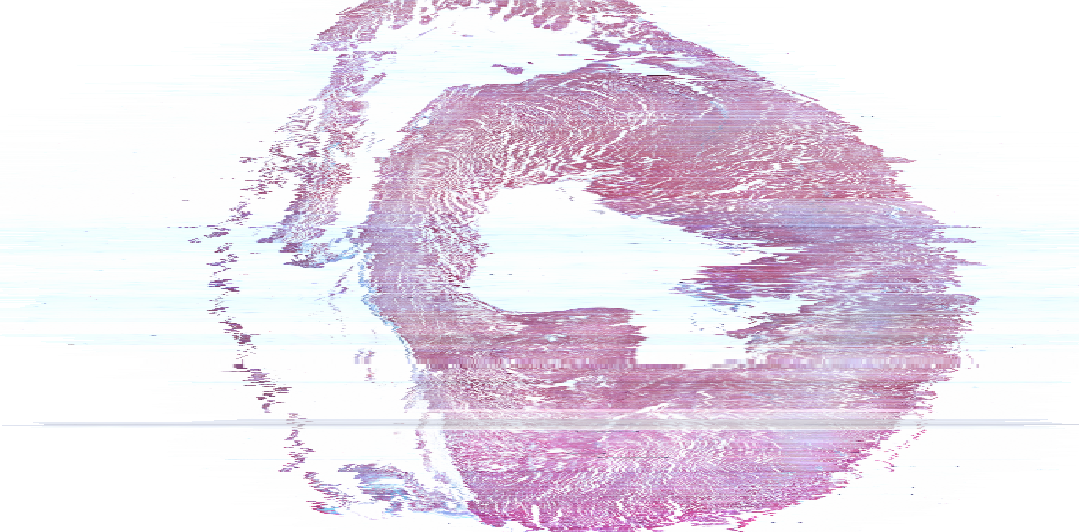
\includegraphics[width=0.9\pagewidth]{Ch7/Figs/banana_1_301}}
      \caption{The full histological volume, registered using the banana method. Even when constrained by a rigid transform, in many areas the slice-to-slice registration is accurate enough that detailed tissue structure is clearly visible. Yet, just as the cylinder does not represent the banana, the resulting geometry of the volume is quite unrelated to ground truth.}
      \label{fig:banana}
    \end{figure}
    
% section aims (end)

\section{Methods} % (fold)
\label{sec:methods}
  Intro: Summary sentence or comment sentence, then list content.

	\subsection{1D Brownian Diffusion} % (fold)
	\label{sub:a_1d_random_walk_analogy}
	  The central limit theorem states that the mean of a sufficiently large number of independent random variables will be approximately normally distributed, regardless of their individual distribution. Indeed, Einstein's theory of the Brownian motion of a diffusive particle is based on this precept. With this in mind, the simplest model of microscopic diffusion is one in which a particle may move in a random walk in one dimension along the integer number line $\mathbb{Z}$, in steps of either $+1$ or $-1$, with equal probability. Taking each step as an independent random variable $Z_1, Z_2,\ldots$, if the particle's position $S$ starts at $S_0 = 0$, we can express the position of the particle after $N$ steps as
	  \begin{equation}
	    S_N = \sum\limits_{i=1}^N Z_i .
	  \end{equation}
	  The probability of taking $k$ positive steps out of a total of $N$ steps is given by
	  \begin{equation}
	    P(k;N) = \binom{N}{k}\left(\frac{1}{2} \right)^N,
	  \end{equation}
	  where the binomial coefficient
	  \begin{equation}
	    \label{eq:registration:binomial-coefficient}
	     \binom{N}{k} = \frac{N!}{k!(N-k)!},
	  \end{equation}
	  since there are $\binom{N}{k}$ possible ways of taking $k$ and $N - k$ steps of $-1$ and $+1$, respectively. At each independent step, the probability of taking one or the other direction is $\frac{1}{2}$, leading to the product $\frac{1}{2}^N$.
  
	  Applying Stirling's approximation:
	  \begin{align}
	    \label{eq:registration:stirling}
	    \ln \left( n! \right) &= n\ln n - n + O(\ln n) \notag \\
	           &\approx n\ln n - n \quad \text{as}\: n \to \infty,
	  \end{align}
  
	  we can see that in the limit of large $N$, the distribution of $k$ and thus $S_N$ tend to Gaussian:
	  \begin{equation}
	    \label{eq:registration:gaussian-approximation}
	    \binom{N}{k}\left(\frac{1}{2}\right)^N \approx \sqrt{\frac{2}{\pi N}} \
	      e^{-2(k - \frac{N}{2})^2/N}.
	  \end{equation}
  
	  \emph{Possibly include proof of de Moivre-Laplace theorem?}
	  % Proof can be found here:
	  % http://en.wikipedia.org/wiki/De_Moivre%E2%80%93Laplace_theorem
  
	  We might consider a concentration of particles $f$ over a discrete 1-dimensional grid $x$. After a discretised timestep $\Delta t$, a proportion $2\alpha$ of the particles have taken one step, such that half of them have diffused to the left and half to the right:
  	
	  \begin{align}
	    f(x_i, t_{n+1}) &= f(x_i, t_n) + \alpha (f(x_{i-1}, t_n) - 2f(x_i, t_n) + f(x_{i+1}, t_n)), \label{eqn:diffusion_1d} \\
	    \frac{\Delta f(x, t + \Delta t)}{\Delta t} &= \alpha (f(x - \Delta x, t) - 2f(x, t) + f(x + \Delta x, t)).
		\end{align}
  	
	  This diffusion will of course act to smooth and homogenise $f$, since regions of high concentration relative to their neighbours will be reduced, and those of low concentration augmented. It is also clear from Equation~\ref{eq:registration:gaussian-approximation} that multiple application of this smoothing operation approximates a Gaussian diffusion smoothing.
		
	% subsection a_1d_random_walk_analogy (end)
	
	\subsection{Simulating 1D Diffusion} % (fold)
	\label{sub:simulating_1d_diffusion}
	  \begin{figure}[htbp]
	    \centering
			\subfigure[][0 iterations]{\includegraphics[width=0.4\pagewidth]{Ch7/Figs/1d_noise/alpha_0.40/000}}
			\subfigure[][1 iterations]{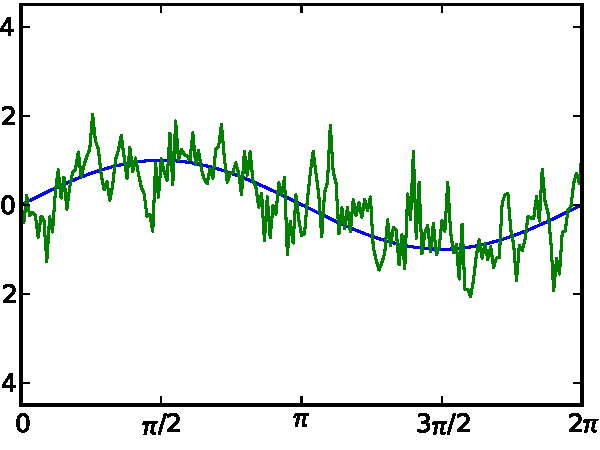
\includegraphics[width=0.4\pagewidth]{Ch7/Figs/1d_noise/alpha_0.40/001}}
			\subfigure[][3 iterations]{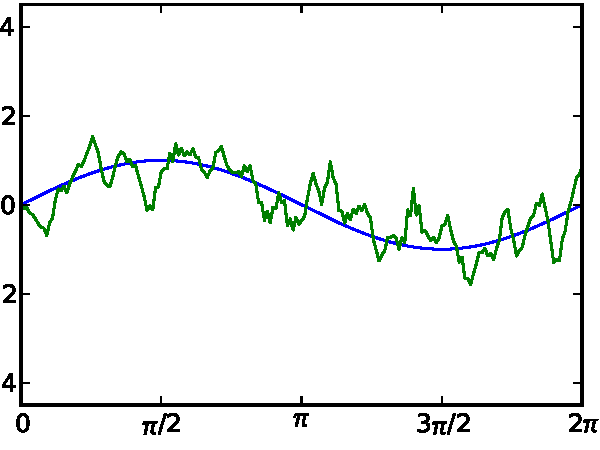
\includegraphics[width=0.4\pagewidth]{Ch7/Figs/1d_noise/alpha_0.40/003}}
			\subfigure[][15 iterations]{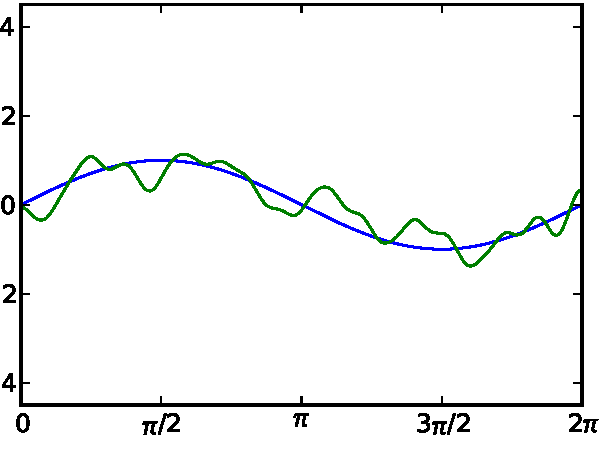
\includegraphics[width=0.4\pagewidth]{Ch7/Figs/1d_noise/alpha_0.40/015}}
			\subfigure[][99 iterations]{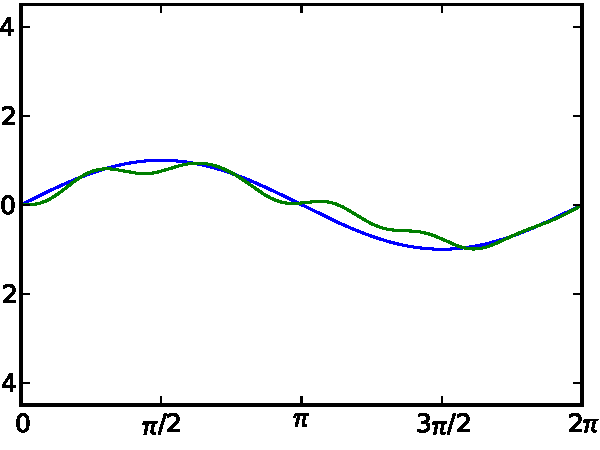
\includegraphics[width=0.4\pagewidth]{Ch7/Figs/1d_noise/alpha_0.40/099}}
			\subfigure[][299 iterations]{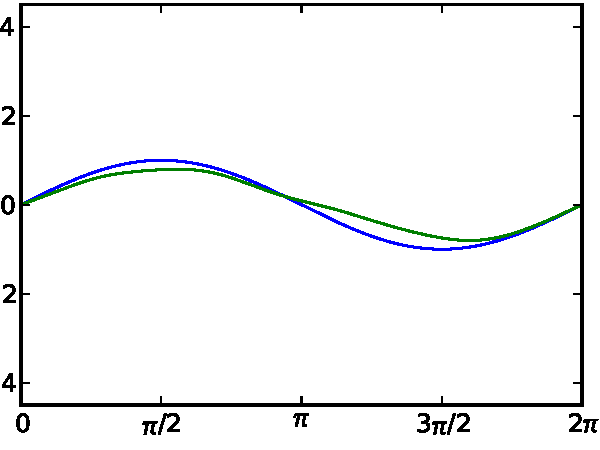
\includegraphics[width=0.4\pagewidth]{Ch7/Figs/1d_noise/alpha_0.40/299}}
	    \caption{A simulation of 1-D diffusion, with $\alpha = 0.4$.}
		  \label{fig:1d_diffusion_0_40}
	  \end{figure}
	
	  \begin{figure}[htbp]
	    \centering
			\subfigure[][0 iterations]{\includegraphics[width=0.4\pagewidth]{Ch7/Figs/1d_noise/alpha_0.49/000}}
			\subfigure[][1 iterations]{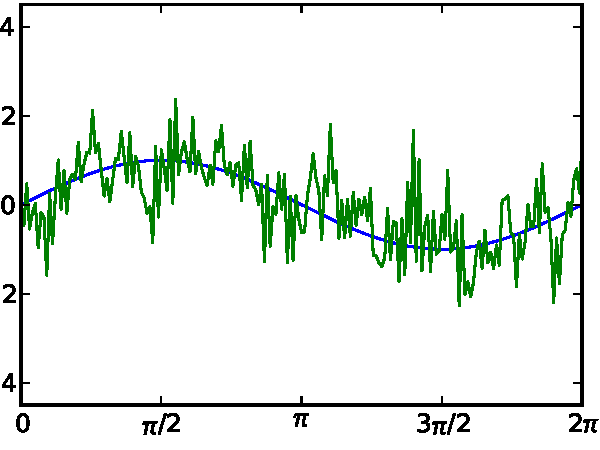
\includegraphics[width=0.4\pagewidth]{Ch7/Figs/1d_noise/alpha_0.49/001}}
			\subfigure[][3 iterations]{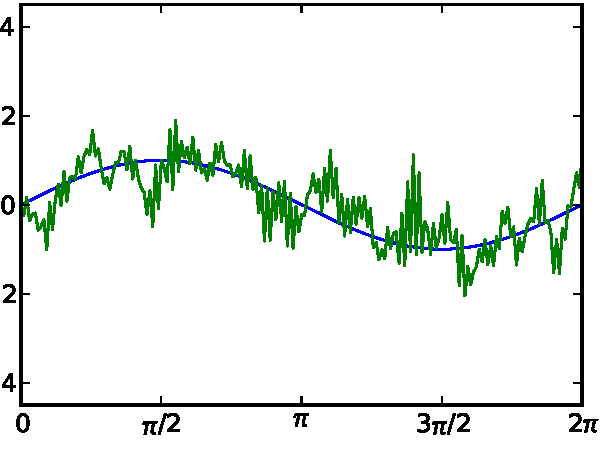
\includegraphics[width=0.4\pagewidth]{Ch7/Figs/1d_noise/alpha_0.49/003}}
			\subfigure[][15 iterations]{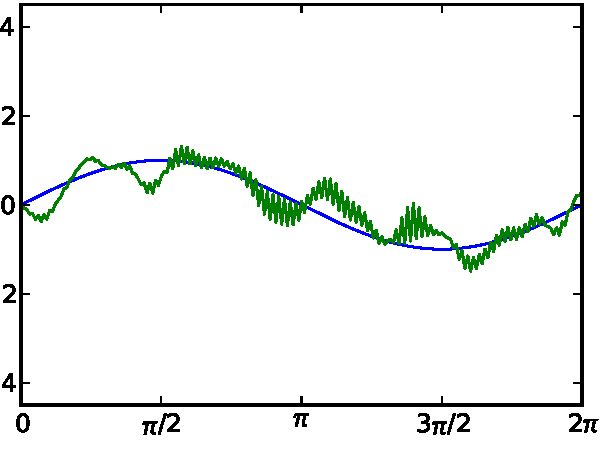
\includegraphics[width=0.4\pagewidth]{Ch7/Figs/1d_noise/alpha_0.49/015}}
			\subfigure[][99 iterations]{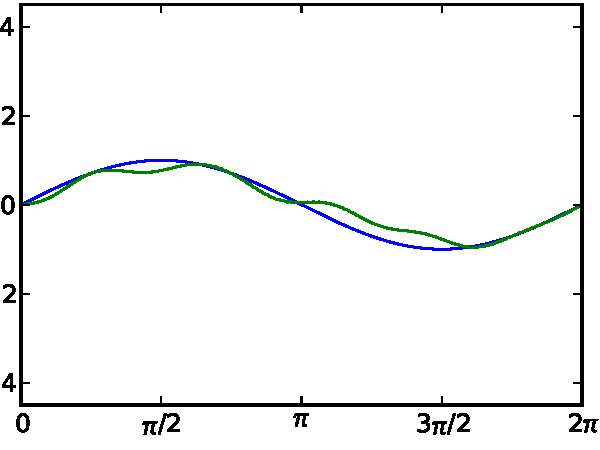
\includegraphics[width=0.4\pagewidth]{Ch7/Figs/1d_noise/alpha_0.49/099}}
			\subfigure[][299 iterations]{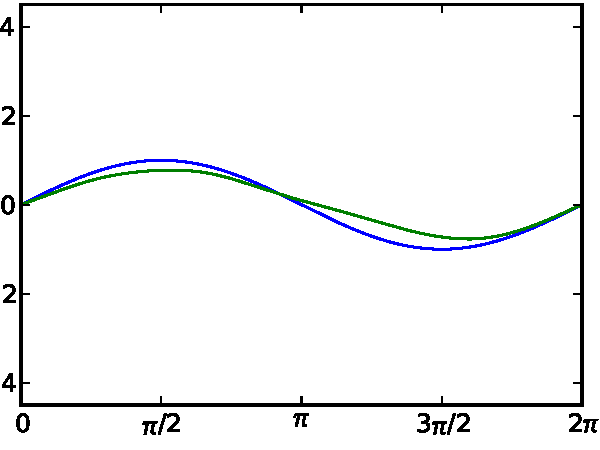
\includegraphics[width=0.4\pagewidth]{Ch7/Figs/1d_noise/alpha_0.49/299}}
	    \caption{A simulation of 1-D diffusion, with $\alpha = 0.49$.}
		  \label{fig:1d_diffusion_0_49}
	  \end{figure}
  
	  \begin{figure}[htbp]
	    \centering
			\subfigure[][0 iterations]{\includegraphics[width=0.4\pagewidth]{Ch7/Figs/1d_noise/alpha_0.50/000}}
			\subfigure[][1 iterations]{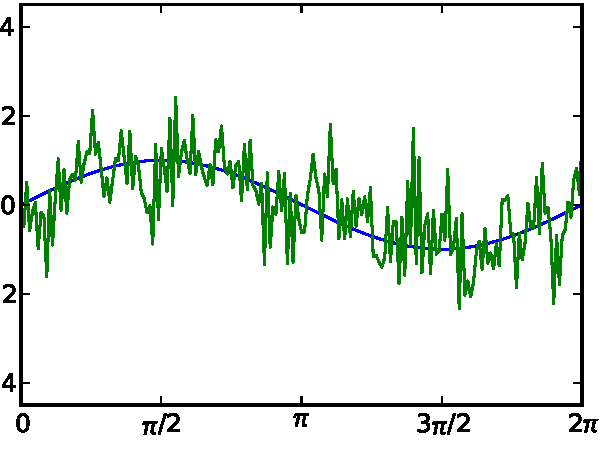
\includegraphics[width=0.4\pagewidth]{Ch7/Figs/1d_noise/alpha_0.50/001}}
			\subfigure[][3 iterations]{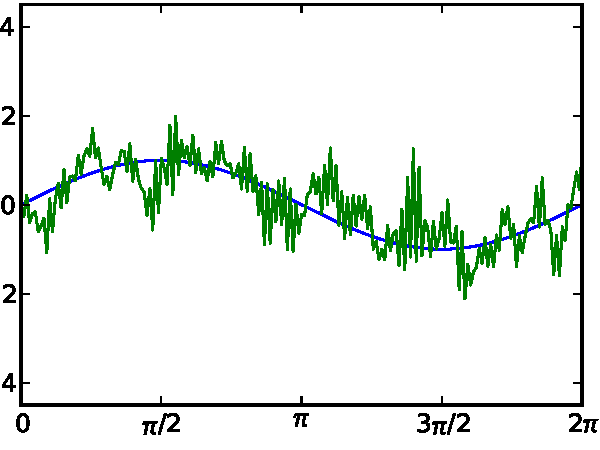
\includegraphics[width=0.4\pagewidth]{Ch7/Figs/1d_noise/alpha_0.50/003}}
			\subfigure[][15 iterations]{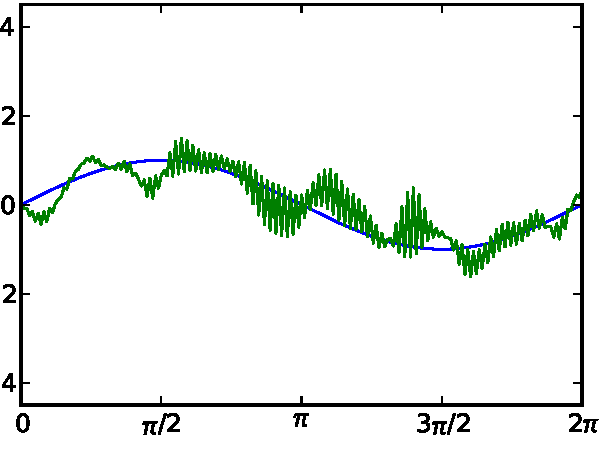
\includegraphics[width=0.4\pagewidth]{Ch7/Figs/1d_noise/alpha_0.50/015}}
			\subfigure[][99 iterations]{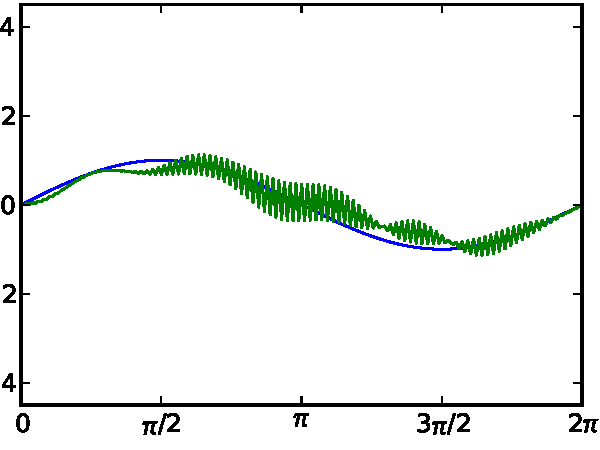
\includegraphics[width=0.4\pagewidth]{Ch7/Figs/1d_noise/alpha_0.50/099}}
			\subfigure[][299 iterations]{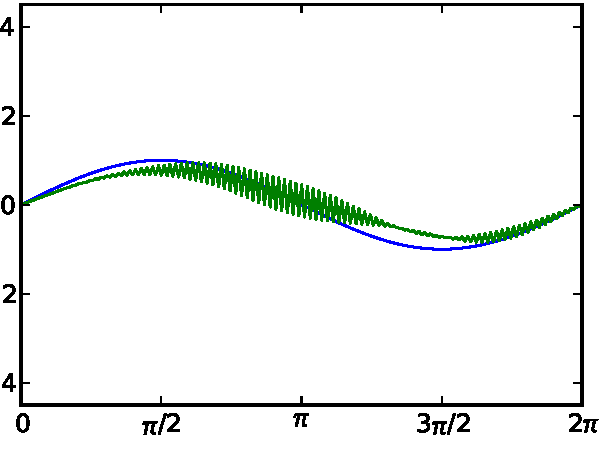
\includegraphics[width=0.4\pagewidth]{Ch7/Figs/1d_noise/alpha_0.50/299}}
	    \caption{A simulation of 1-D diffusion, with $\alpha = 0.5$.}
		  \label{fig:1d_diffusion_0_50}
	  \end{figure}
  
	  \begin{figure}[htbp]
	    \centering
	  	\subfigure[][0 iterations]{\includegraphics[width=0.4\pagewidth]{Ch7/Figs/1d_noise/alpha_0.51/000}}
	  	\subfigure[][1 iterations]{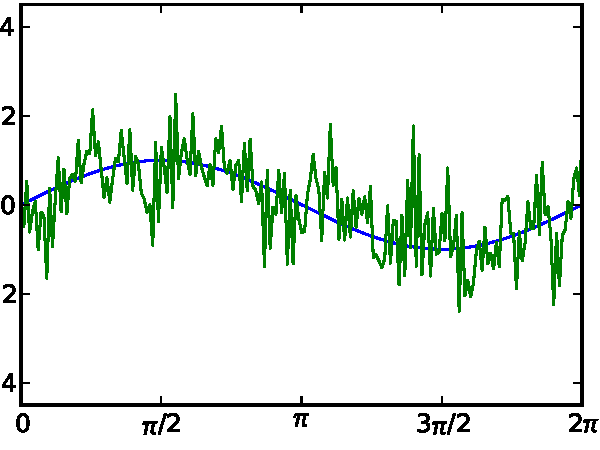
\includegraphics[width=0.4\pagewidth]{Ch7/Figs/1d_noise/alpha_0.51/001}}
	  	\subfigure[][3 iterations]{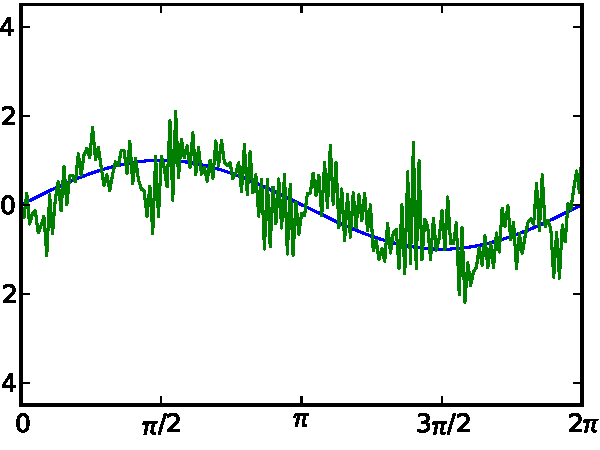
\includegraphics[width=0.4\pagewidth]{Ch7/Figs/1d_noise/alpha_0.51/003}}
	  	\subfigure[][15 iterations]{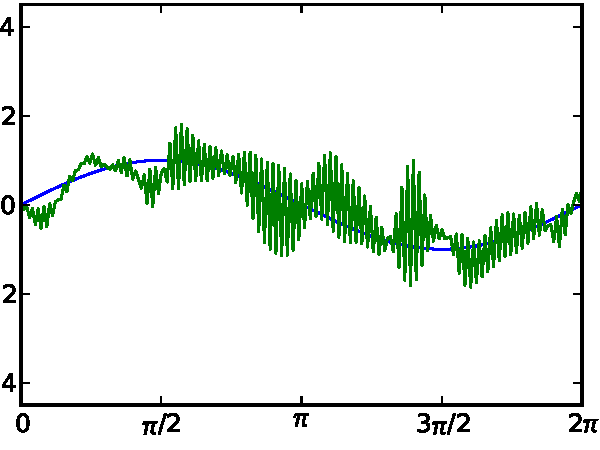
\includegraphics[width=0.4\pagewidth]{Ch7/Figs/1d_noise/alpha_0.51/015}}
	  	\subfigure[][99 iterations]{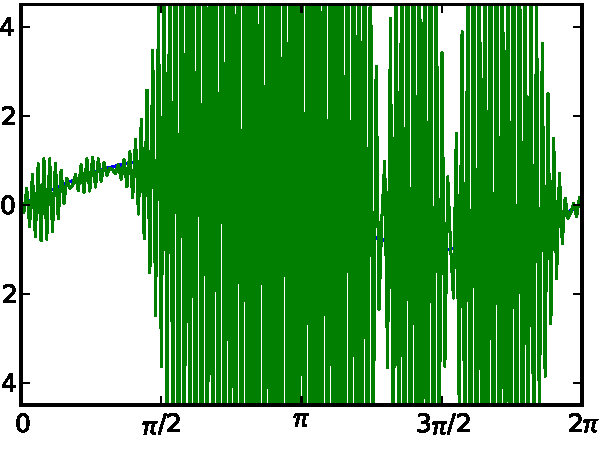
\includegraphics[width=0.4\pagewidth]{Ch7/Figs/1d_noise/alpha_0.51/099}}
	  	\subfigure[][299 iterations]{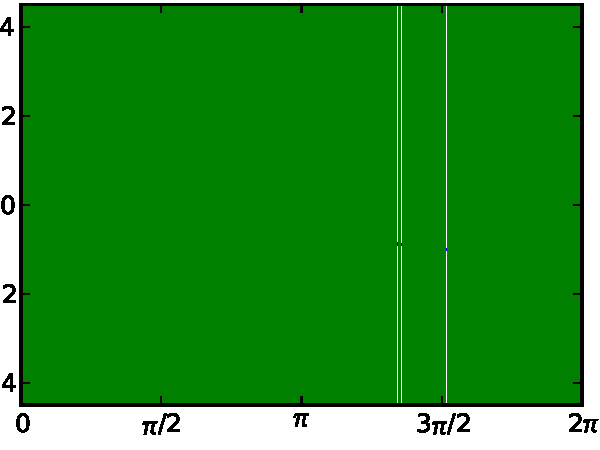
\includegraphics[width=0.4\pagewidth]{Ch7/Figs/1d_noise/alpha_0.51/299}}
	    \caption{A simulation of 1-D diffusion, with $\alpha = 0.51$.}
	    \label{fig:1d_diffusion_0_51}
	  \end{figure}
  
	
	
	  This process can be simulated quite trivially. A numerical approximation of a sine wave is graphed in blue in each of Figures~\labelcref{fig:1d_diffusion_0_40,fig:1d_diffusion_0_49,fig:1d_diffusion_0_50,fig:1d_diffusion_0_51}, on 200 equispaced points from $0$ to $2\pi$. Random noise from a Gaussian distribution is added, with variance equal to the amplitude of the sine wave, and is plotted in green. The subfigures show the evolution of the noise after 0, 1, 3, 15, 99 and 299 timesteps.
  
	  Our purpose is to smooth out the high frequency random noise from the green wave as quickly and as computationally cheaply as is possible, whilst maintaining the underlying low frequency signal. There is a tradeoff to be made when deciding upon a value for $\alpha$. The greater $\alpha$, the more particles move to the left and right at each iteration, and so the faster the noise is damped. But when $\alpha$ approaches 0.5, almost all of the particles from each bin are moving out at each iteration, and unstable oscillations start to appear. In Figure~\ref{fig:1d_diffusion_0_40}, $\alpha$ is set to 0.4, a great compromise between speed of smoothing and stability. $\alpha$ is set to 0.49 in Figure~\ref{fig:1d_diffusion_0_49}, and the highest frequency is actually damped much more slowly, as oscillatory `swapping' effects start to appear. When $\alpha = 0.5$ in Figure~\ref{fig:1d_diffusion_0_50}, the highest frequency is still undamped after 300 iterations, and by the time $\alpha$ is at 0.51 in Figure~\ref{fig:1d_diffusion_0_51}, the system is unstable. This is not entirely surprising, since it is unphysical for more than all of the particles to diffuse out of a particular bin at each timestep.
	% subsection simulating_1d_diffusion (end)
		
	\subsection{Transformational Diffusion} % (fold)
	\label{sub:transformational_diffusion}
	  An ITK transform $\mathbf{T}$ acting on a point $\mathbf{p}$ maps points in the resampling space to points in the original image space:
		
		\begin{equation}
			\mathbf{p'} = \mathbf{Tp}
		\end{equation}
		
		Our goal is to develop an iterative process that `diffuses' each slice toward its neighbours. At iteration $n$ of this process, each slice $i$ in a reconstructed histological stack has associated with it an invertible transform $\mathbf{T}_i^n$. We define the transform $\mathbf{\Delta T}_i^{n,n+1}$, which is pre-applied to a point in the resampling space of $i$ before $\mathbf{T}_i^n$, such that
		
		\begin{equation}
			\mathbf{T}_i^{n+1} = \mathbf{T}_i^n \mathbf{\Delta T}_i^{n,n+1}.
		\end{equation}
		
	  How would this $\mathbf{\Delta T}_i^{n,n+1}$ be defined? In the case of 1-dimensional diffusion, we can reformulate the right hand side of Equation~\ref{eqn:diffusion_1d} into two separate terms thusly:
		
	  \begin{align}
	    f(x_i, t_{n+1}) &= f(x_i, t_n) + \alpha ((f(x_{i+1}, t_n) - f(x_i, t_n)) - (f(x_{i-1}, t_n) - f(x_i, t_n)) \\
			\Delta f_i^{n,n+1} &= \alpha (\Delta f_{i,i+1}^n - \Delta f_{i-1,i}^n) \\
			                   &= \alpha \Delta f_{i,i-1}^n + \alpha \Delta f_{i,i+1}^n, \label{eqn:1d_diffusion_operator}
		\end{align}
		
    where $\Delta f_i^{m,n}$ is the difference in $f$ at position $i$ between timestep $m$ and timestep $n$, and $\Delta f_{i,j}^m$ is the difference in $f$ between position $i$ and position $j$ at timestep $m$. From Equation~\ref{eqn:1d_diffusion_operator}, we can see that at each timestep, the concentration at each bin moves towards its left and right neighbour by a proportion $\alpha$ of its difference from each, respectively.
		
	  We might, then, propose analogously that
		
		\begin{equation}
		 	\mathbf{\Delta T}_i^{n,n+1} = \alpha \cdot \mathbf{\Delta T}_{i,i+1}^n \oplus \alpha \cdot \mathbf{\Delta T}_{i,i-1}^n, \label{eqn:transformational_placeholder}
		\end{equation}
	 	
	 	where $\mathbf{\Delta T}_{i,j}^n$ is defined as the transformation that registers a histological slice $i$ to slice $j$ at iteration $n$, $\cdot$ is a placeholder for a binary operator on a scalar and a transform, and $\oplus$ is a placeholder for a binary operator on a pair of transforms. The question now emerges: what precise form do the two binary operators take? We will start by outlining their desirable properties, and then discuss implementations that satisfy these constraints.
		
		The operator $\cdot$ takes two operands: a scalar and a transform. We would like $0$ to be the null operand on $\mathbf{T}$, so that when $\alpha = 0$, no diffusion occurs. We would like $1$ to be the identity operand on $\mathbf{T}$, so that when $\alpha = 1$, the transform from each term in \ref{eqn:transformational_placeholder} would diffuse the slice exactly to the position of its equivalent neighbour. Ideally, we would also like addition of the scalar operand to distribute over the serial application of the resultant transforms, so that transforms vary smoothly and naturally with respect to the scalar operand. For example, in the case of a 2-dimensional rotation matrix, the rotation angle would vary proportionally with the scalar operand. This final condition can be satisfied for certain transforms, such as linear transforms and vector field transforms, but cannot be satisfied in general for others, such as b-spline transforms. To summarise in mathematical form, we would like the following to hold:
		
		\begin{align}
			0 \cdot \mathbf{T} &= \mathbf{I} \label{eqn:null} \\
			1 \cdot \mathbf{T} &= \mathbf{T} \label{eqn:identity} \\
			(\alpha \cdot \mathbf{T}) (\beta \cdot \mathbf{T}) &= (\alpha + \beta) \cdot \mathbf{T} \label{eqn:distributivity}
		\end{align}
	 	
	  The operator $\oplus$ takes two transform operands. Commutativity must hold if the diffusion is to be symmetric i.e. behave identically if the order of the slices is reversed. That is,
		
		\begin{equation}
			\forall \mathbf{S}, \mathbf{T} : \mathbf{S} \oplus \mathbf{T} = \mathbf{T} \oplus \mathbf{S}. \label{eqn:commutativity}
		\end{equation}
		
		Unfortunately, commutativity rules out the straightforward serial application of transforms. For example, in the general case of matrix multiplication, $AB \ne BA$. One solution is to use the transform that is equivalent to returning the Euclidian midpoint of $\mathbf{Sp}$ and $\mathbf{Tp}$ for all $\mathbf{p}$, but again, this may not always be representable by some types of transform. In the case of rotation matrices, it seems sensible to return the mean of the two angles; and for similarity transforms, the geometric mean of the two enlargement factors. Inductively therefore, the operator $\oplus$ would do well to return the midpoint of some appropriate parameterisation of the operand transforms.
		
	  It is elucidating to apply this general mathematical form to concrete classes of transform, in order of increasing complexity: translation transforms, rotation transforms, similarity transforms, affine transforms and more general deformable transforms. An ITK affine transform $\mathbf{T}$ acting on a point $\mathbf{p}$ consists of a matrix transformation $\mathbf{M}$, followed by a translation by an offset vector $\mathbf{o}$:
		
		\begin{equation}
			\mathbf{p'} = \mathbf{Tp}= \mathbf{Mp} + \mathbf{o}.
		\end{equation}
		
		In the simplest case of translation transforms, where $\mathbf{M}$ is the identity matrix $\mathbf{I}$, the two translation parameters are independent and individually identical to the 1-dimensional diffusion in \ref{eqn:1d_diffusion_operator}. Operator $\cdot$ is a scalar multiplication of each offset parameter, and operator $\oplus$ is the commutative serial application of the transforms (or equivalently, addition of the respective parameters):
		
		\begin{align}
			(\alpha \cdot \mathbf{T}) \mathbf{p} &= \mathbf{p} + \alpha\mathbf{o} \\
			(\mathbf{S} \oplus \mathbf{T}) \mathbf{p} &= \mathbf{STp} \\
			                                          &= \mathbf{p} + \mathbf{o_S} + \mathbf{o_T}
		\end{align}
		
		Clearly, these two operators satisfy \labelcref{eqn:null,eqn:identity,eqn:distributivity,eqn:commutativity}. Equation~\ref{eqn:transformational_placeholder} becomes
		
		\begin{align}
		 	\mathbf{\Delta T}_i^{n,n+1} \mathbf{p} &= (\alpha \mathbf{\Delta T}_{i,i-1}^n) (\alpha \mathbf{\Delta T}_{i,i+1}^n) \mathbf{p} \\
			\mathbf{p} + \mathbf{o}_i^{n,n+1} &= \mathbf{p} + \alpha \mathbf{o}_{i,i-1}^n + \alpha \mathbf{o}_{i,i+1}^n \\
			\mathbf{o}_i^{n,n+1} &= \alpha (\mathbf{o}_{i,i-1}^n + \mathbf{o}_{i,i+1}^n) 
		\end{align}
		
		The offsets are therefore trivially analogous to \ref{eqn:1d_diffusion_operator}.
		
		In the case of rigid transforms, $\mathbf{M}$ is a rotation matrix
		
		\begin{equation}
			\mathbf{R}(\theta) = \left( \begin{matrix}
			  										 \cos \theta & -\sin\theta \\
														 \sin\theta & \cos\theta
					                 \end{matrix} \right) .
		\end{equation}
		
		In 2 dimensions, rotation matrices commute, and the result of their multiplication is simply a rotation matrix with angle equal to the sum of the operands' angles; in the special case where there are no offsets, then serial application of the transforms is a candidate for operator $\oplus$ according to \ref{eqn:commutativity}:
		
		\begin{equation}
			\mathbf{S} \oplus \mathbf{T} = \mathbf{R}(\theta_\mathbf{S})\mathbf{R}(\theta_\mathbf{T}) = \mathbf{R}(\theta_\mathbf{S} + \theta_\mathbf{T})
		\end{equation}
		
		
		In a similar vein, an operator $\cdot$ that multiplies the angle of the input transform with $\alpha$ fulfils criteria \labelcref{eqn:null,eqn:identity,eqn:distributivity}:
    
    \begin{equation}
      \alpha \cdot \mathbf{T} = R(\alpha\theta)
    \end{equation}
		
		When offsets are introduced, however, commutativity no longer holds and criteria \labelcref{eqn:distributivity,eqn:commutativity} are not fulfilled:
		
		
		In the case of rigid transforms, $\mathbf{M}$ is a rotation matrix $\mathbf{R}$ multiplied by an enlargement $\sigma$. 
		
		In most practical applications of this method, where the slices are already roughly coherent, the registration transforms between neighbouring slices $T_{i,i+1}^n$ are close to the identity transform. It is therefore interesting to examine how the various implementations of the two operators $\cdot$ and $\oplus$ behave in the small limit.
	
	% subsection transformational_diffusion (end)
	
  % colour slice differences
  \begin{figure}[htbp]
    \centering
    \subfigure[][unperturbed image]{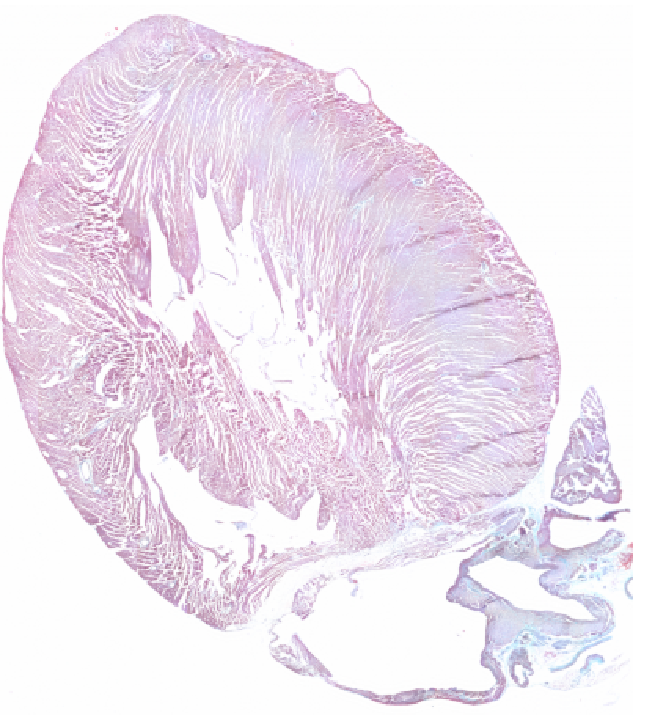
\includegraphics[height=0.365\textheight,type=pdf,ext=.pdf,read=.pdf]{Ch7/Figs/dummies/colour_perfect_slice}} \quad
    \subfigure[][image with transformational noise]{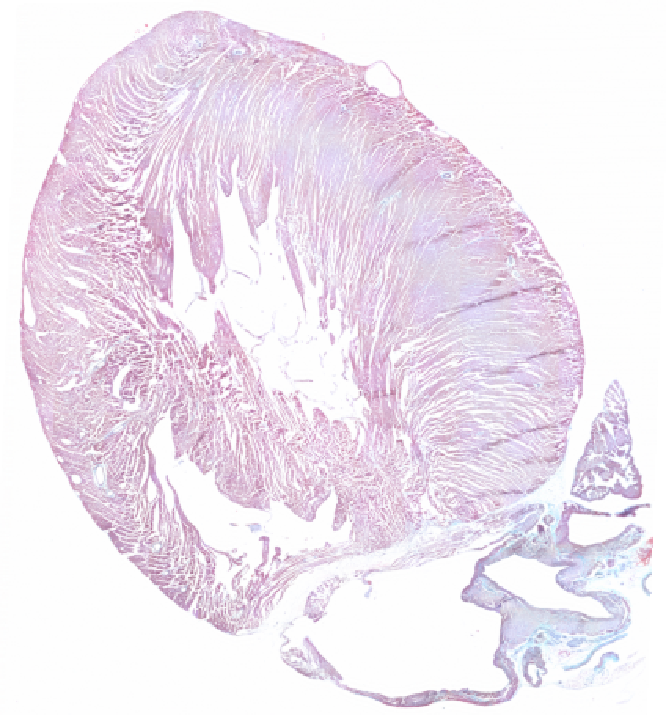
\includegraphics[height=0.365\textheight,type=pdf,ext=.pdf,read=.pdf]{Ch7/Figs/dummies/colour_noisy_slice}} \\
    \subfigure[][squared differences in intensities]{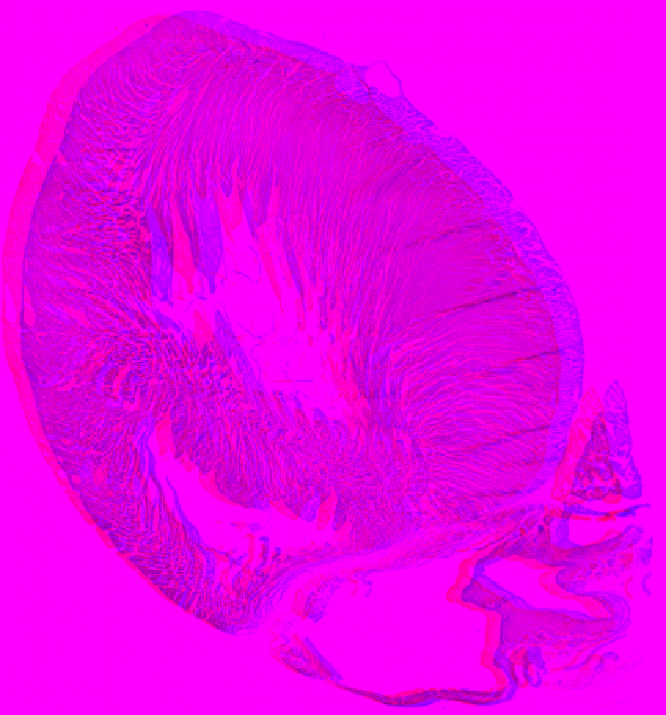
\includegraphics[height=0.365\textheight,type=pdf,ext=.pdf,read=.pdf]{Ch7/Figs/dummies/colour_red_blue_diff}} \quad
    \subfigure[][squared differences in intensities]{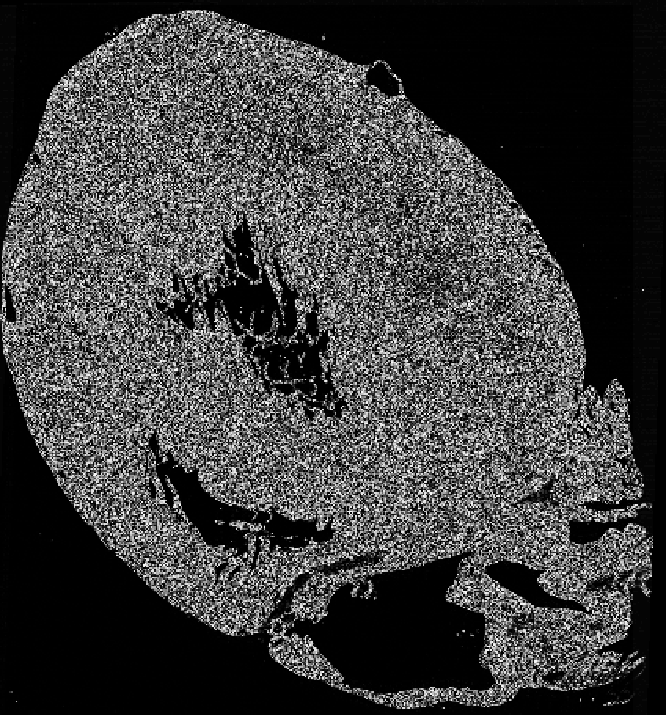
\includegraphics[height=0.365\textheight,type=pdf,ext=.pdf,read=.pdf]{Ch7/Figs/dummies/colour_squared_diff}}
    \caption{slice 99 of straight volume. mean squared difference in bw image: 61.5265135808}
    \label{fig:dummy_cross_sections}
  \end{figure}
  
  % segmentation slice differences
  \begin{figure}[htbp]
    \centering
    \subfigure[][unperturbed image]{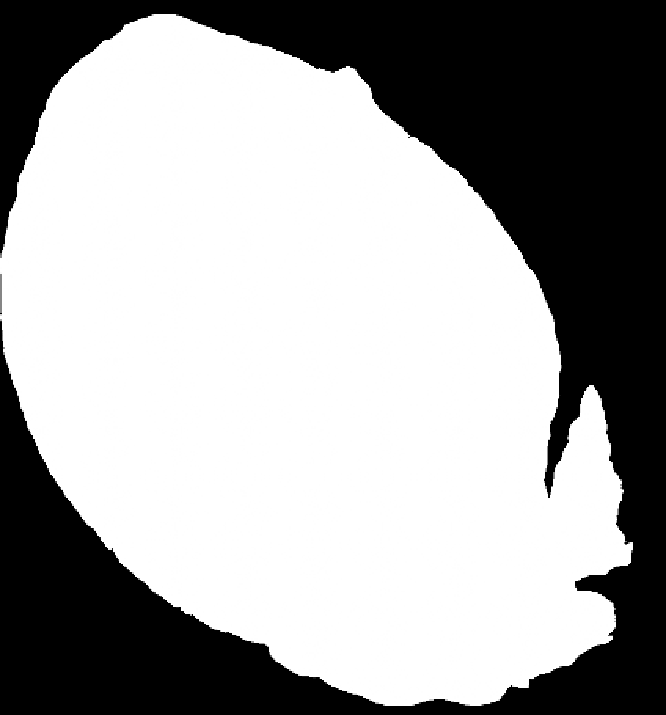
\includegraphics[height=0.365\textheight,type=pdf,ext=.pdf,read=.pdf]{Ch7/Figs/dummies/segmentation_perfect_slice}} \quad
    \subfigure[][image with transformational noise]{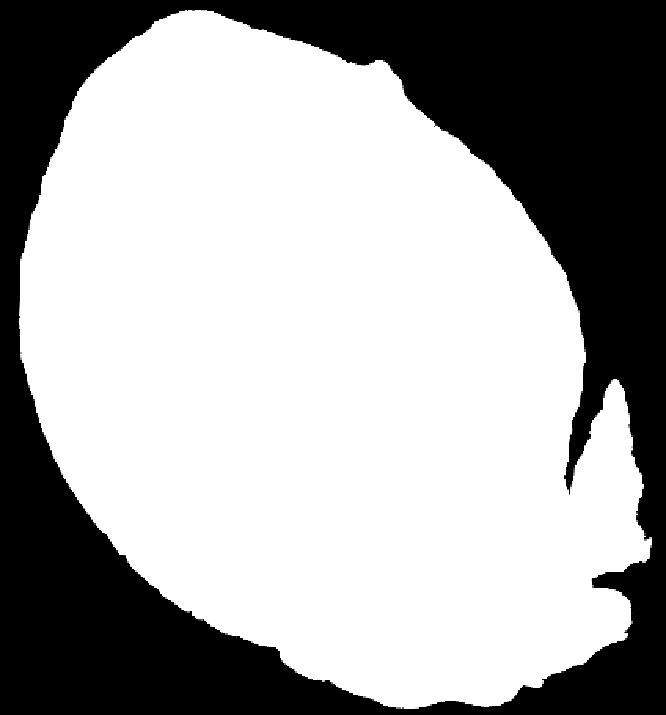
\includegraphics[height=0.365\textheight,type=pdf,ext=.pdf,read=.pdf]{Ch7/Figs/dummies/segmentation_noisy_slice}} \\
    \subfigure[][squared differences in intensities]{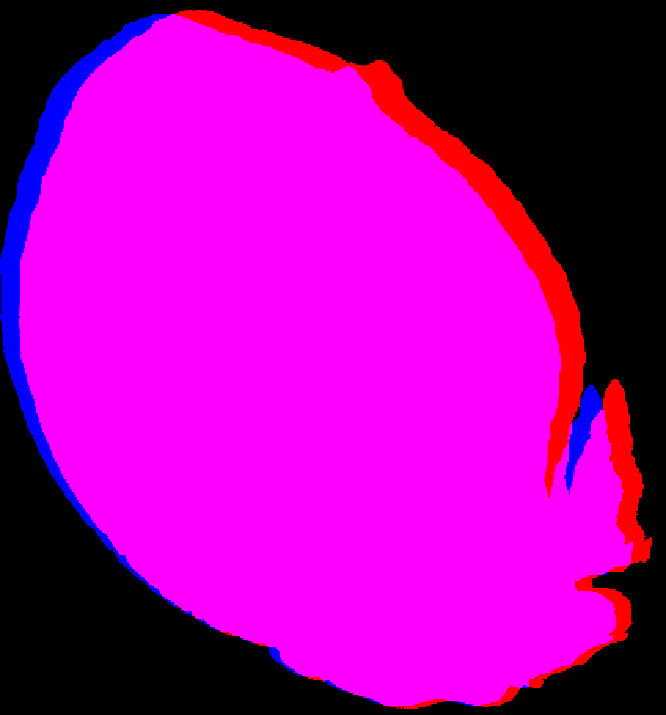
\includegraphics[height=0.365\textheight,type=pdf,ext=.pdf,read=.pdf]{Ch7/Figs/dummies/segmentation_red_blue_diff}} \quad
    \subfigure[][squared differences in intensities]{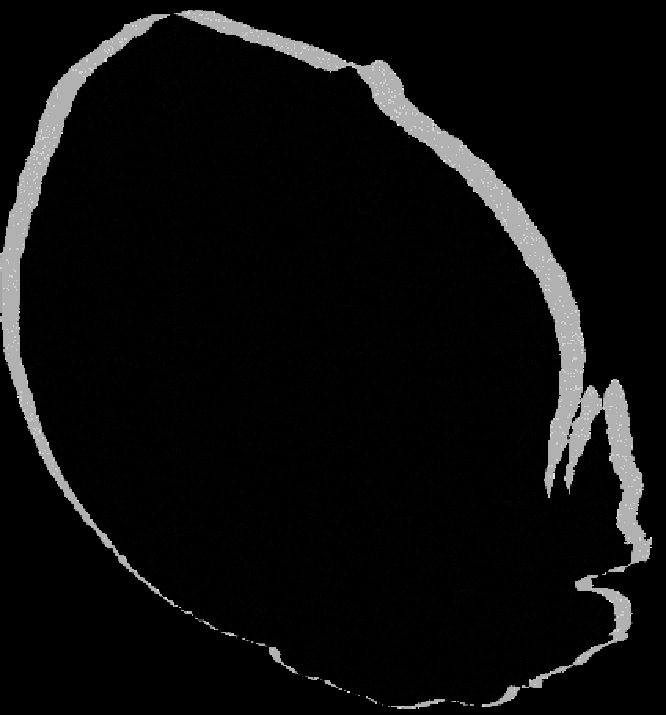
\includegraphics[height=0.365\textheight,type=pdf,ext=.pdf,read=.pdf]{Ch7/Figs/dummies/segmentation_squared_diff}}
    \caption{slice 99 of straight volume, reconstructed using manual segmentation. mean squared difference in bw image: 12.9321}
    \label{fig:dummy_cross_sections}
  \end{figure}
  
  % straight
  \begin{figure}[htbp]
    \centering
    % filename format: cross_section_200_alpha0.4_ITERATION_DIMENSION_SLICE
    \subfigure[][with noise (0 iterations)]{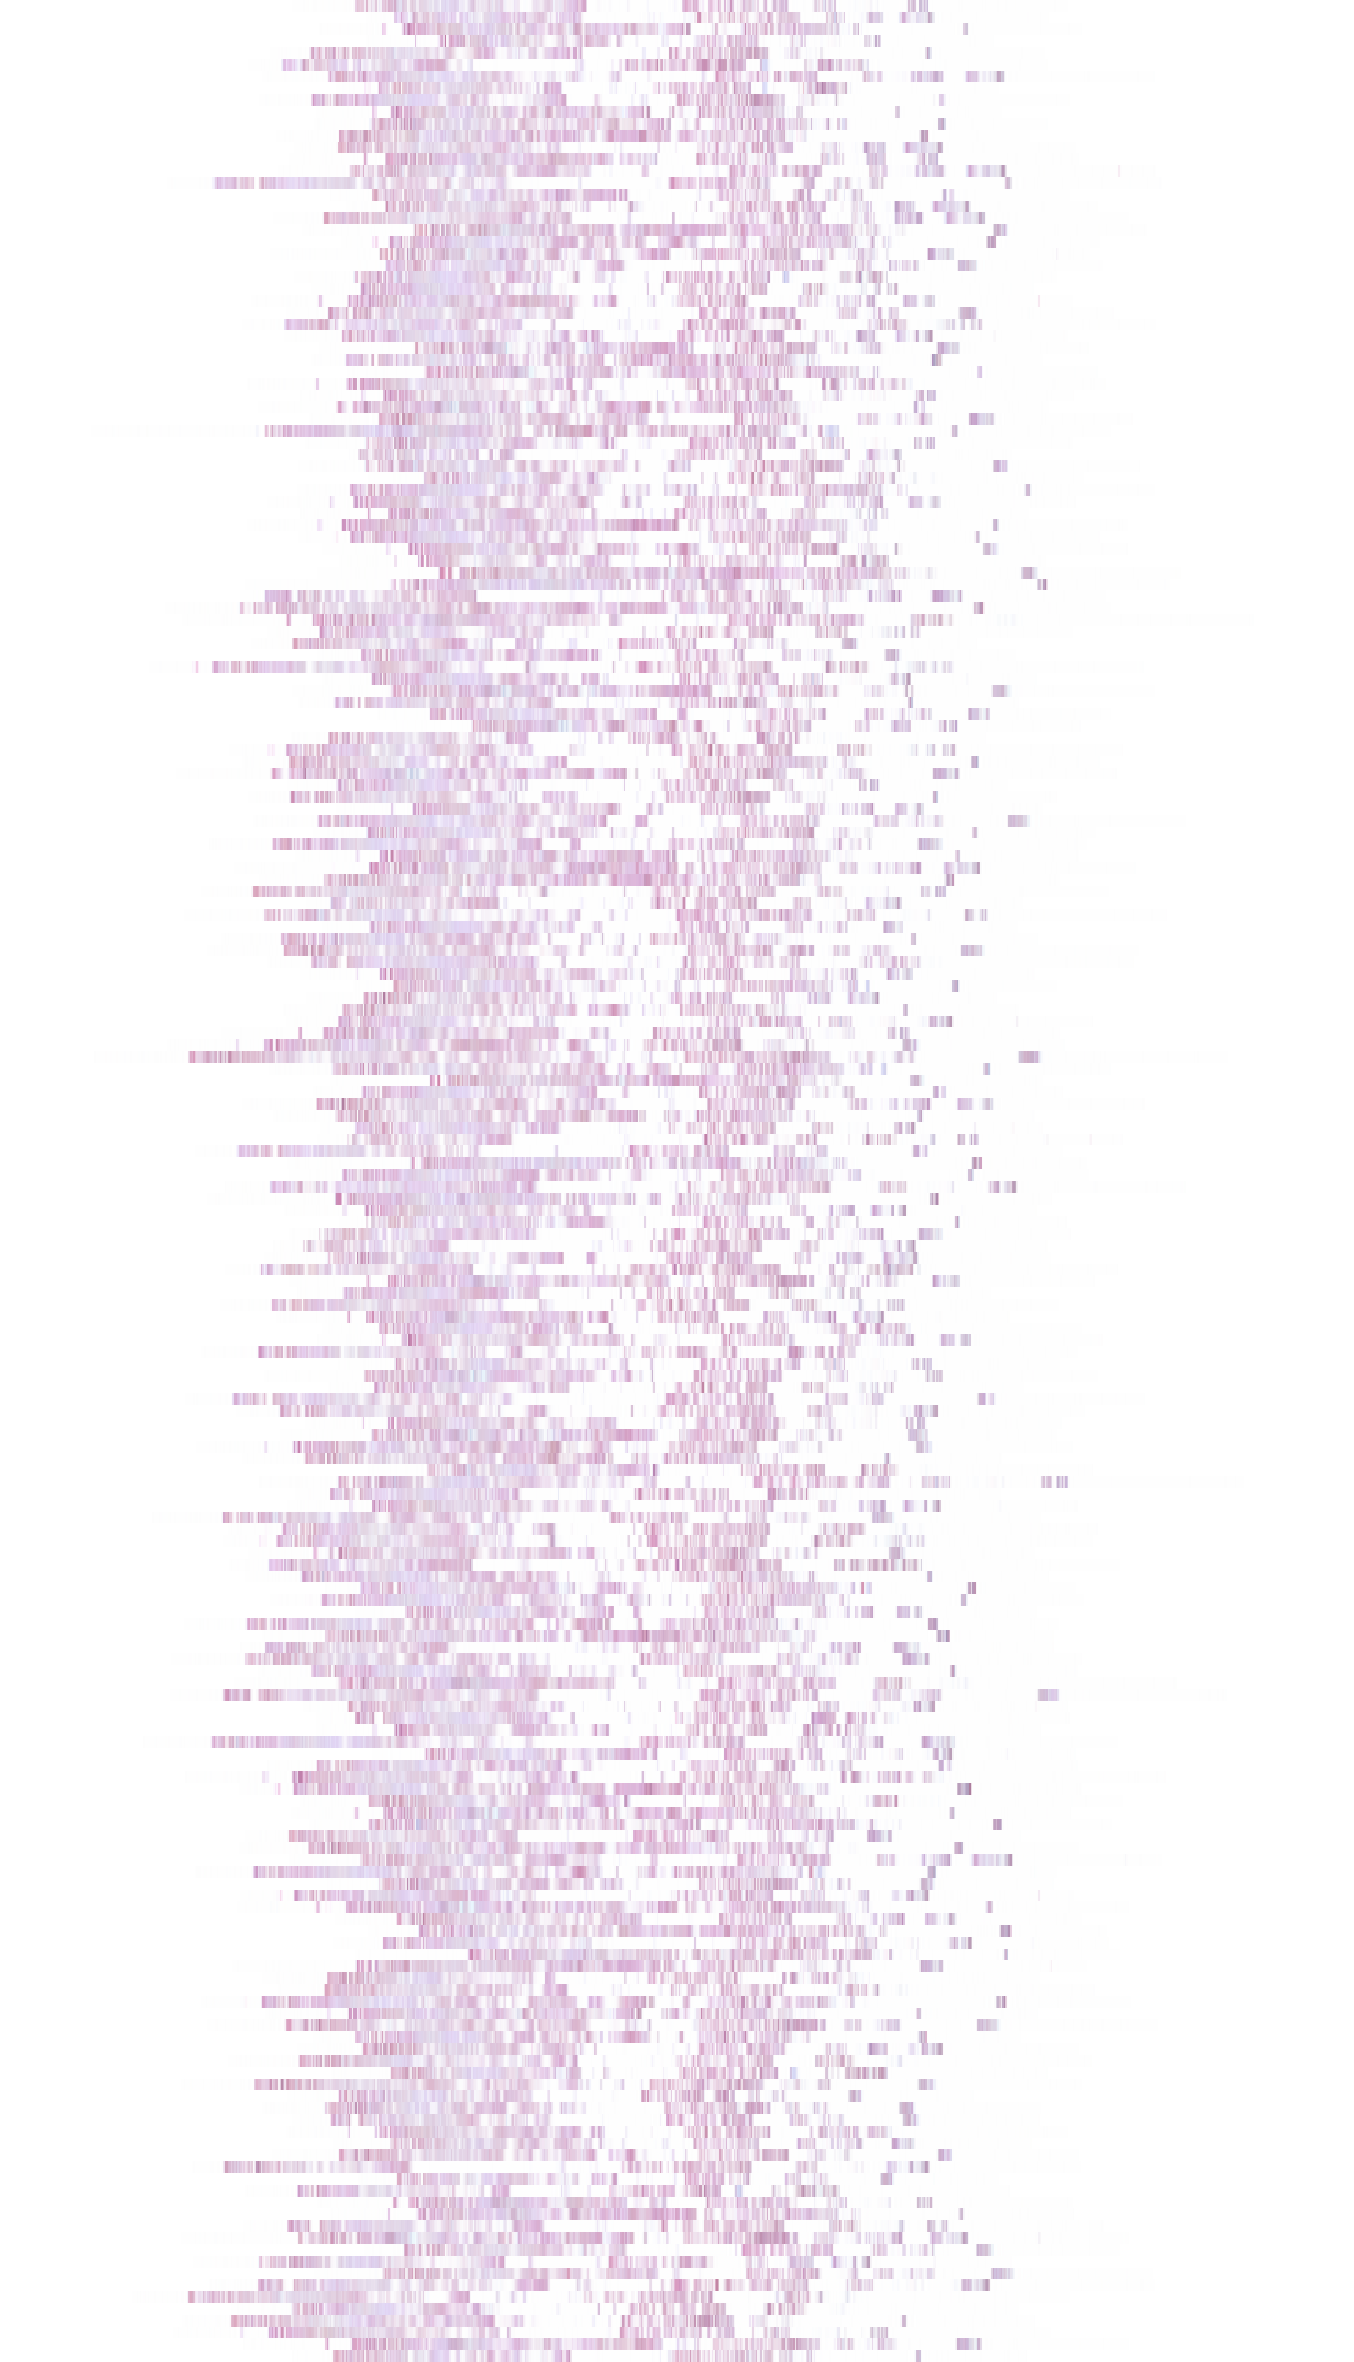
\includegraphics[height=0.4\textheight,type=pdf,ext=.pdf,read=.pdf]{Ch7/Figs/dummies/cross_section_200_alpha0.4_0_0_352}\label{fig:subfig1}}
    \subfigure[][1 iteration]{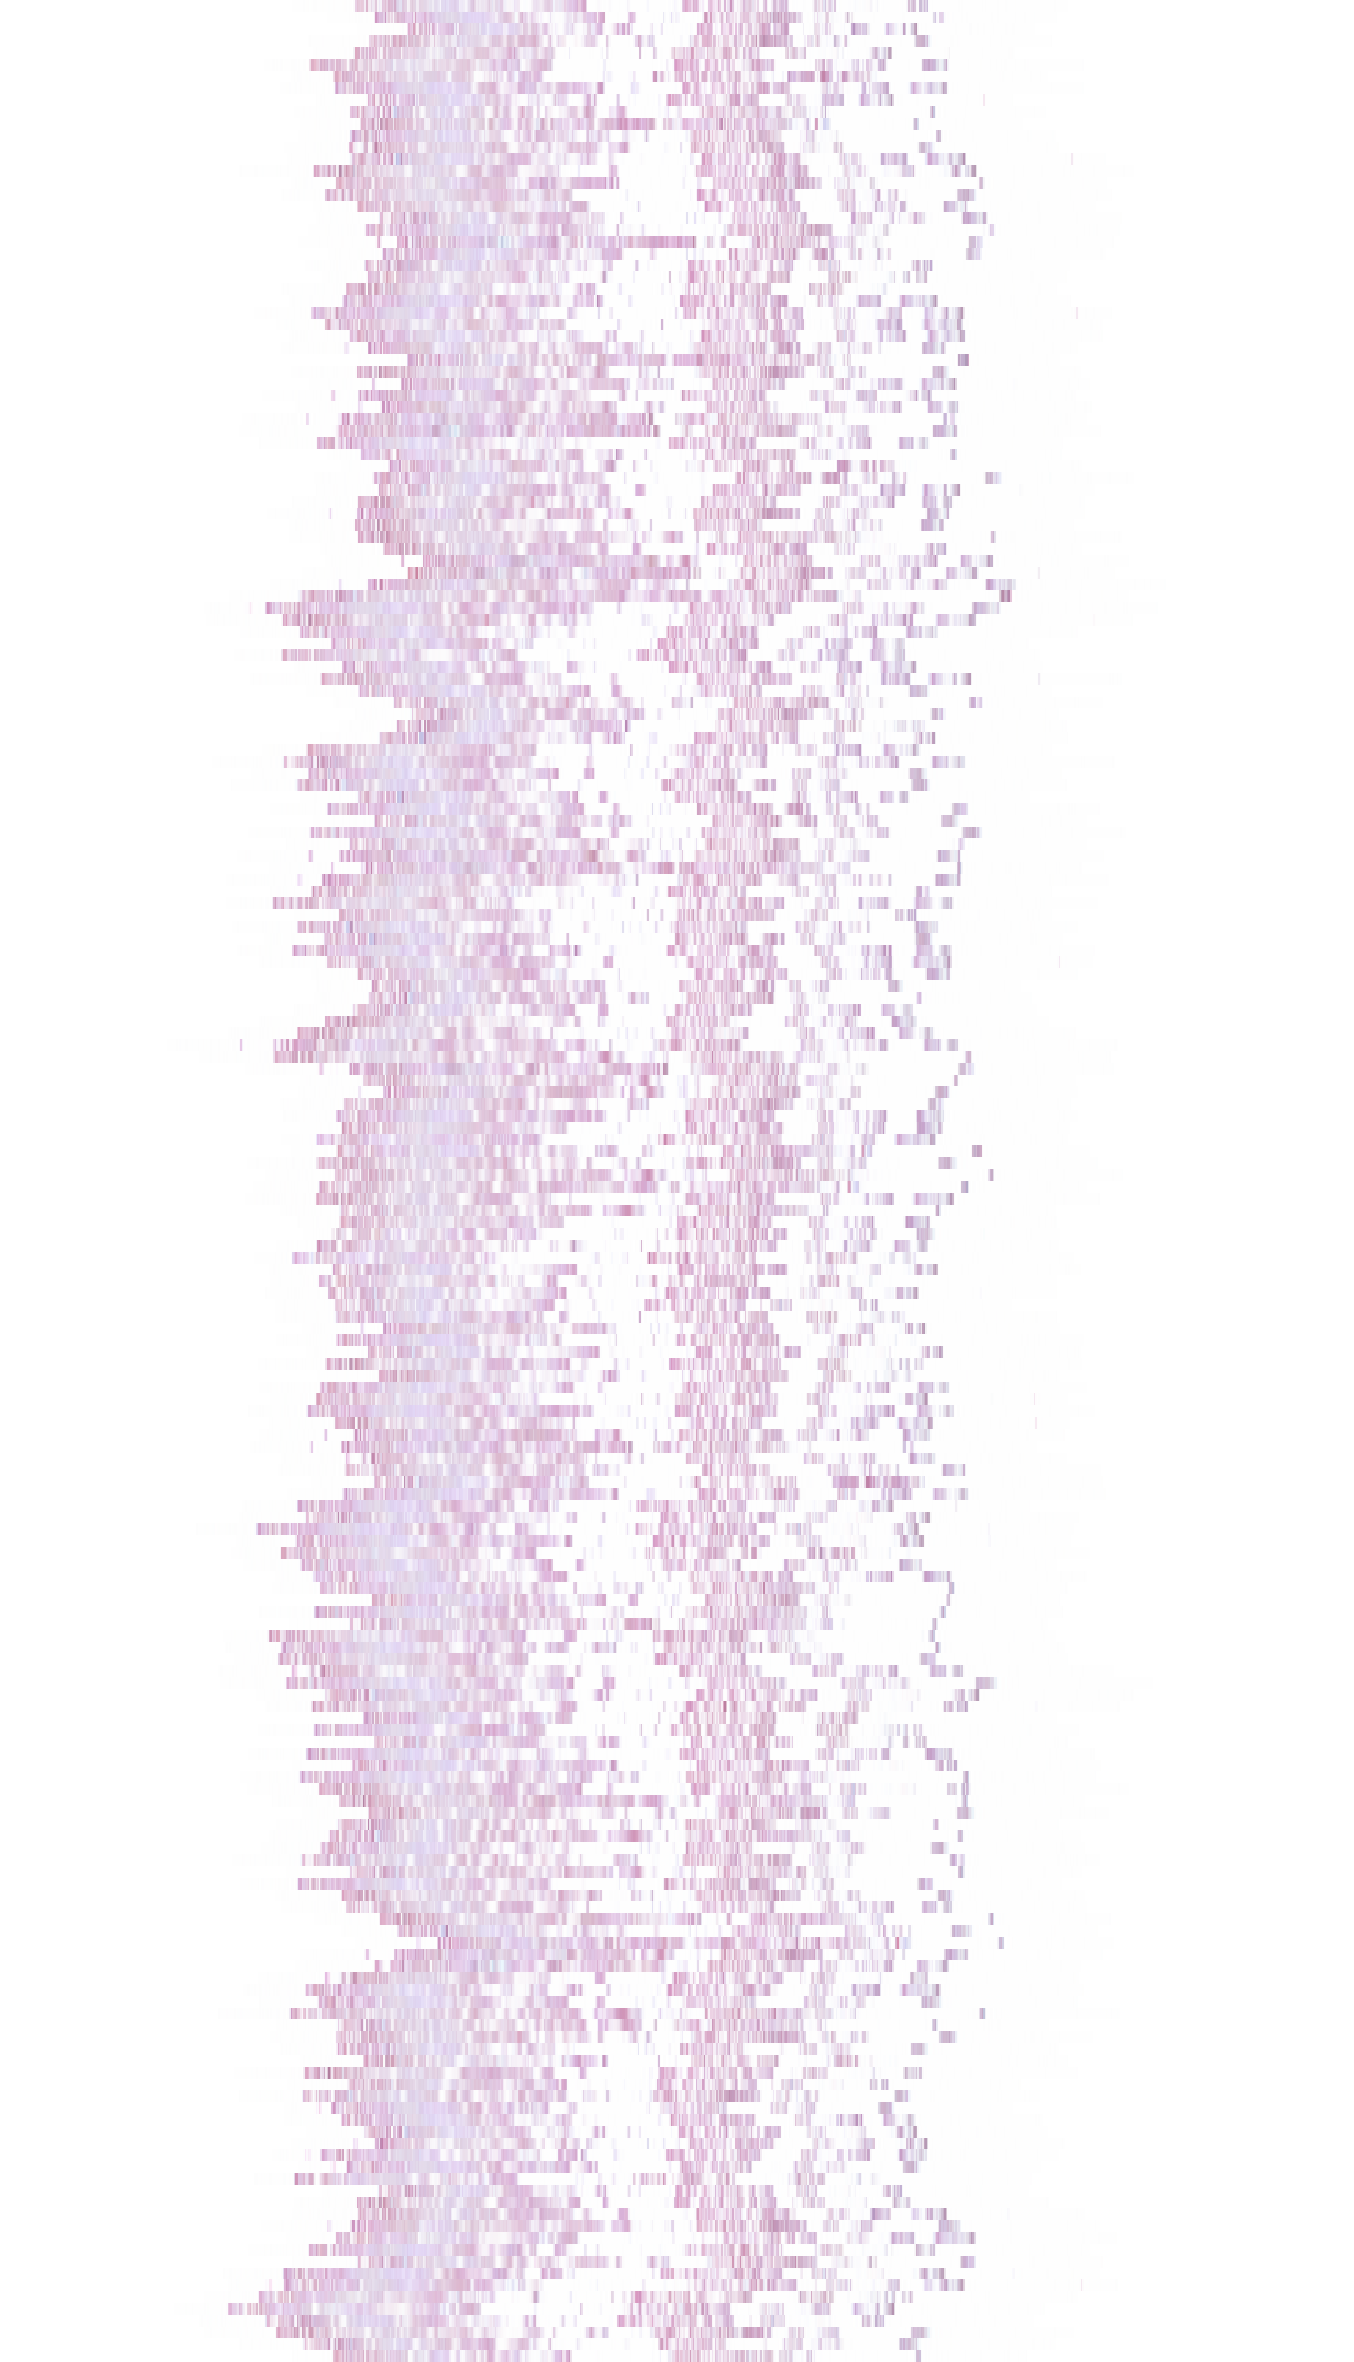
\includegraphics[height=0.4\textheight,type=pdf,ext=.pdf,read=.pdf]{Ch7/Figs/dummies/cross_section_200_alpha0.4_1_0_352}\label{fig:subfig2}}
    \subfigure[][3 iterations]{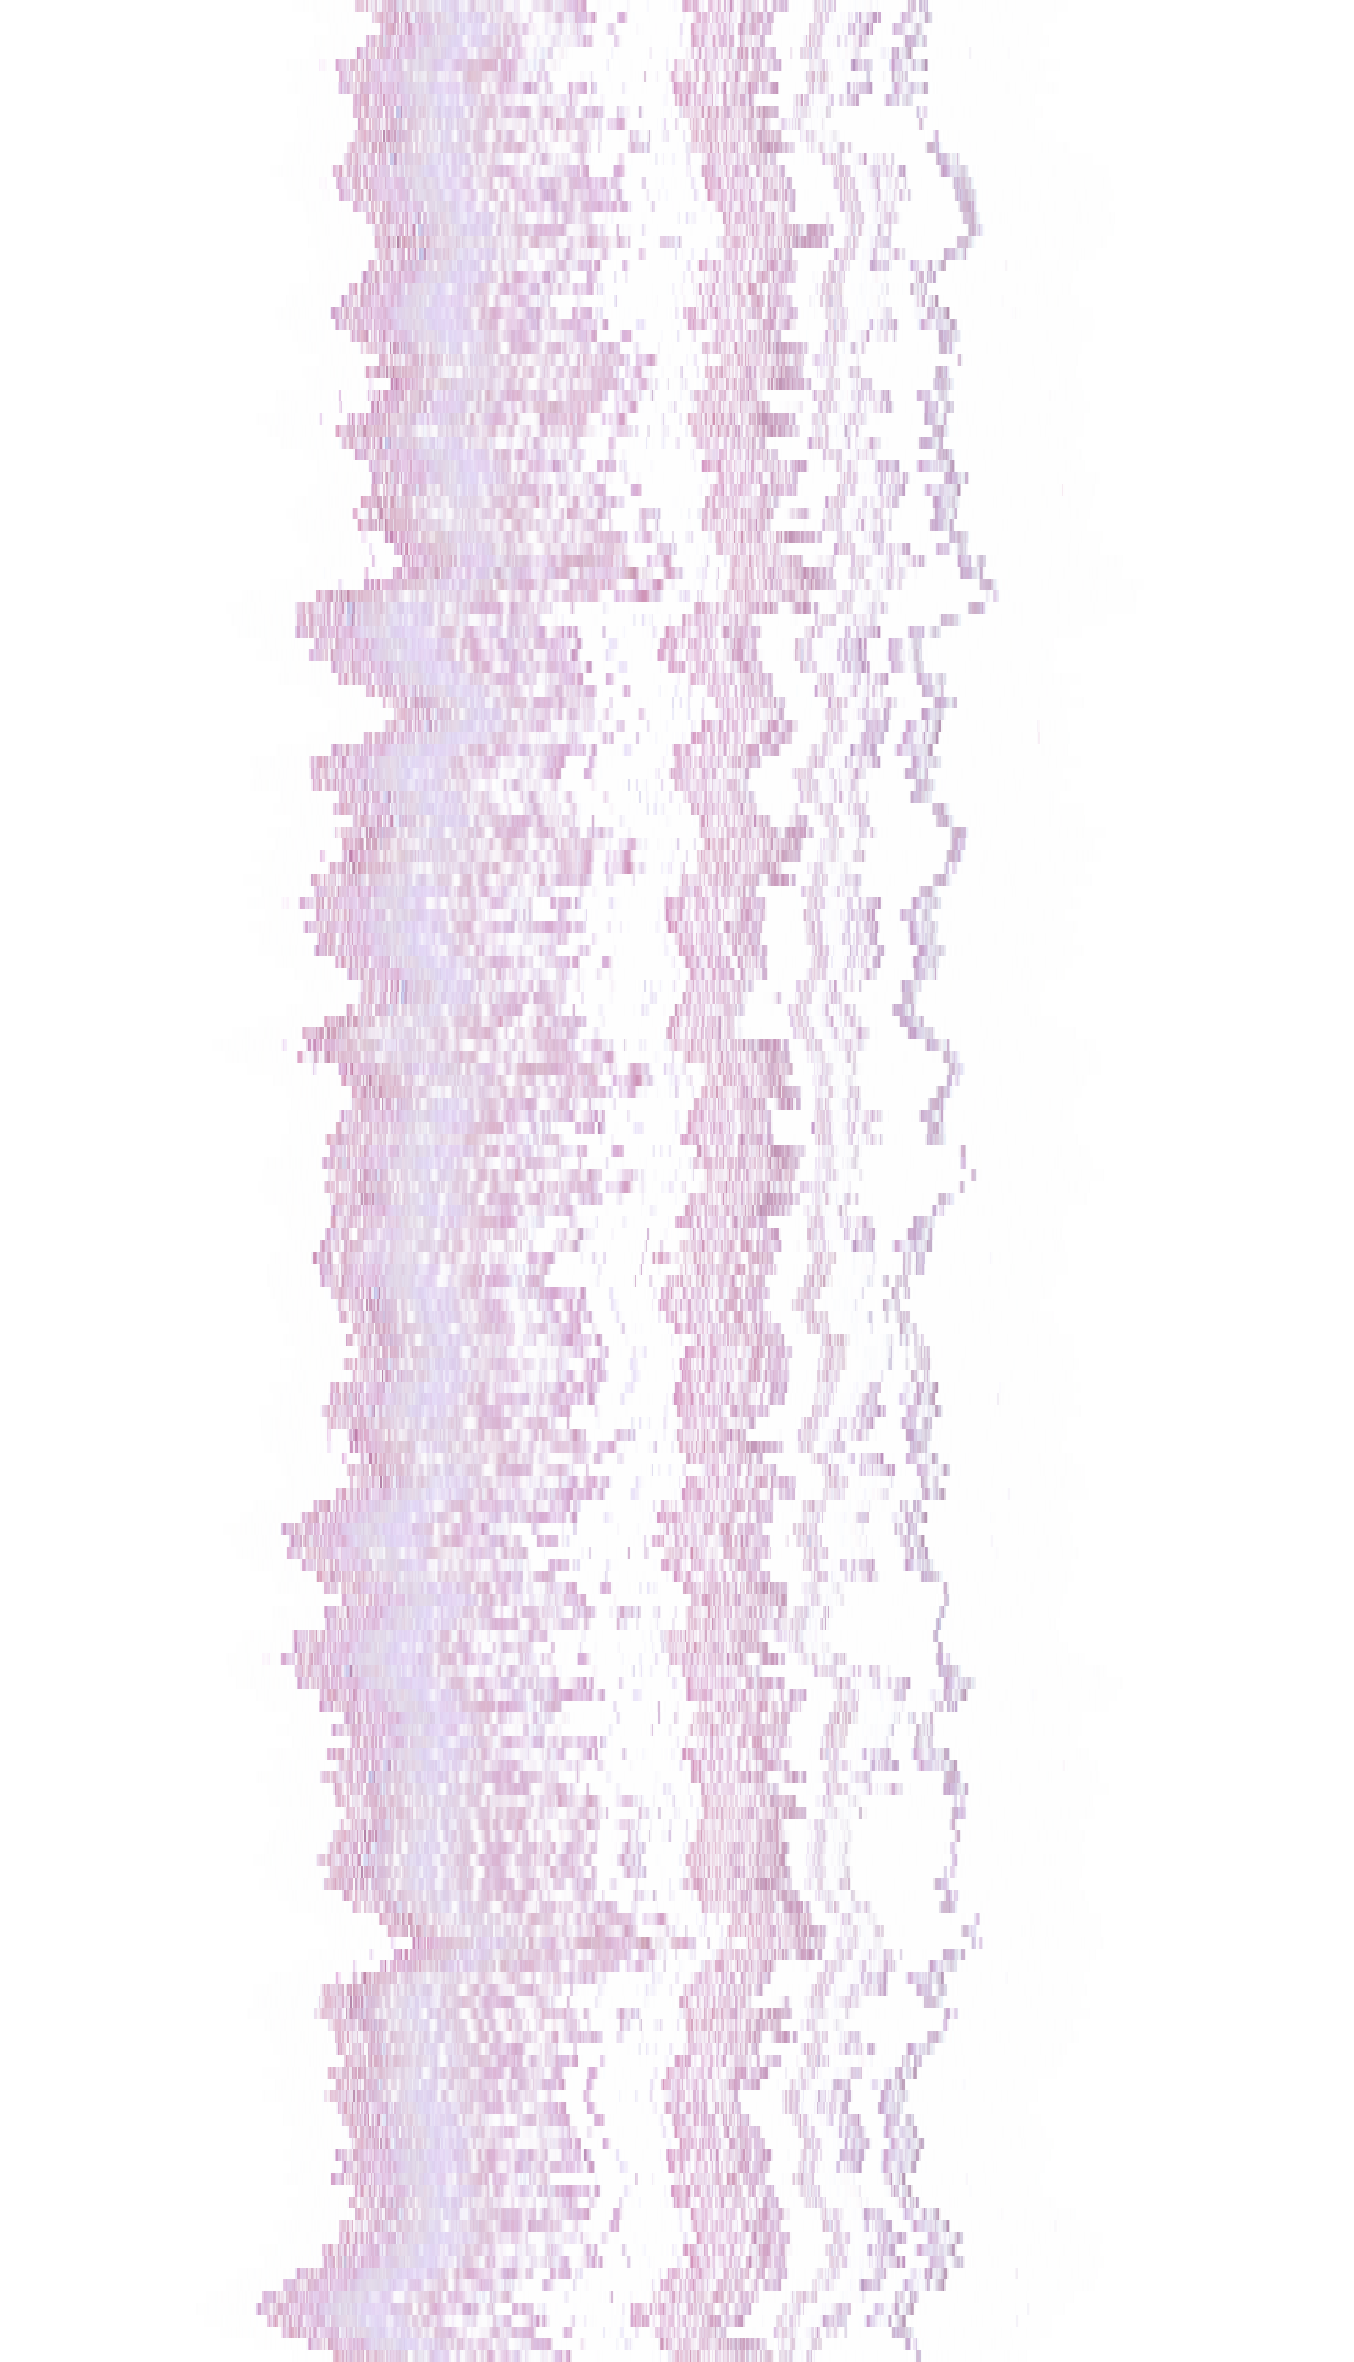
\includegraphics[height=0.4\textheight,type=pdf,ext=.pdf,read=.pdf]{Ch7/Figs/dummies/cross_section_200_alpha0.4_3_0_352}\label{fig:subfig3}}
    \subfigure[][8 iterations]{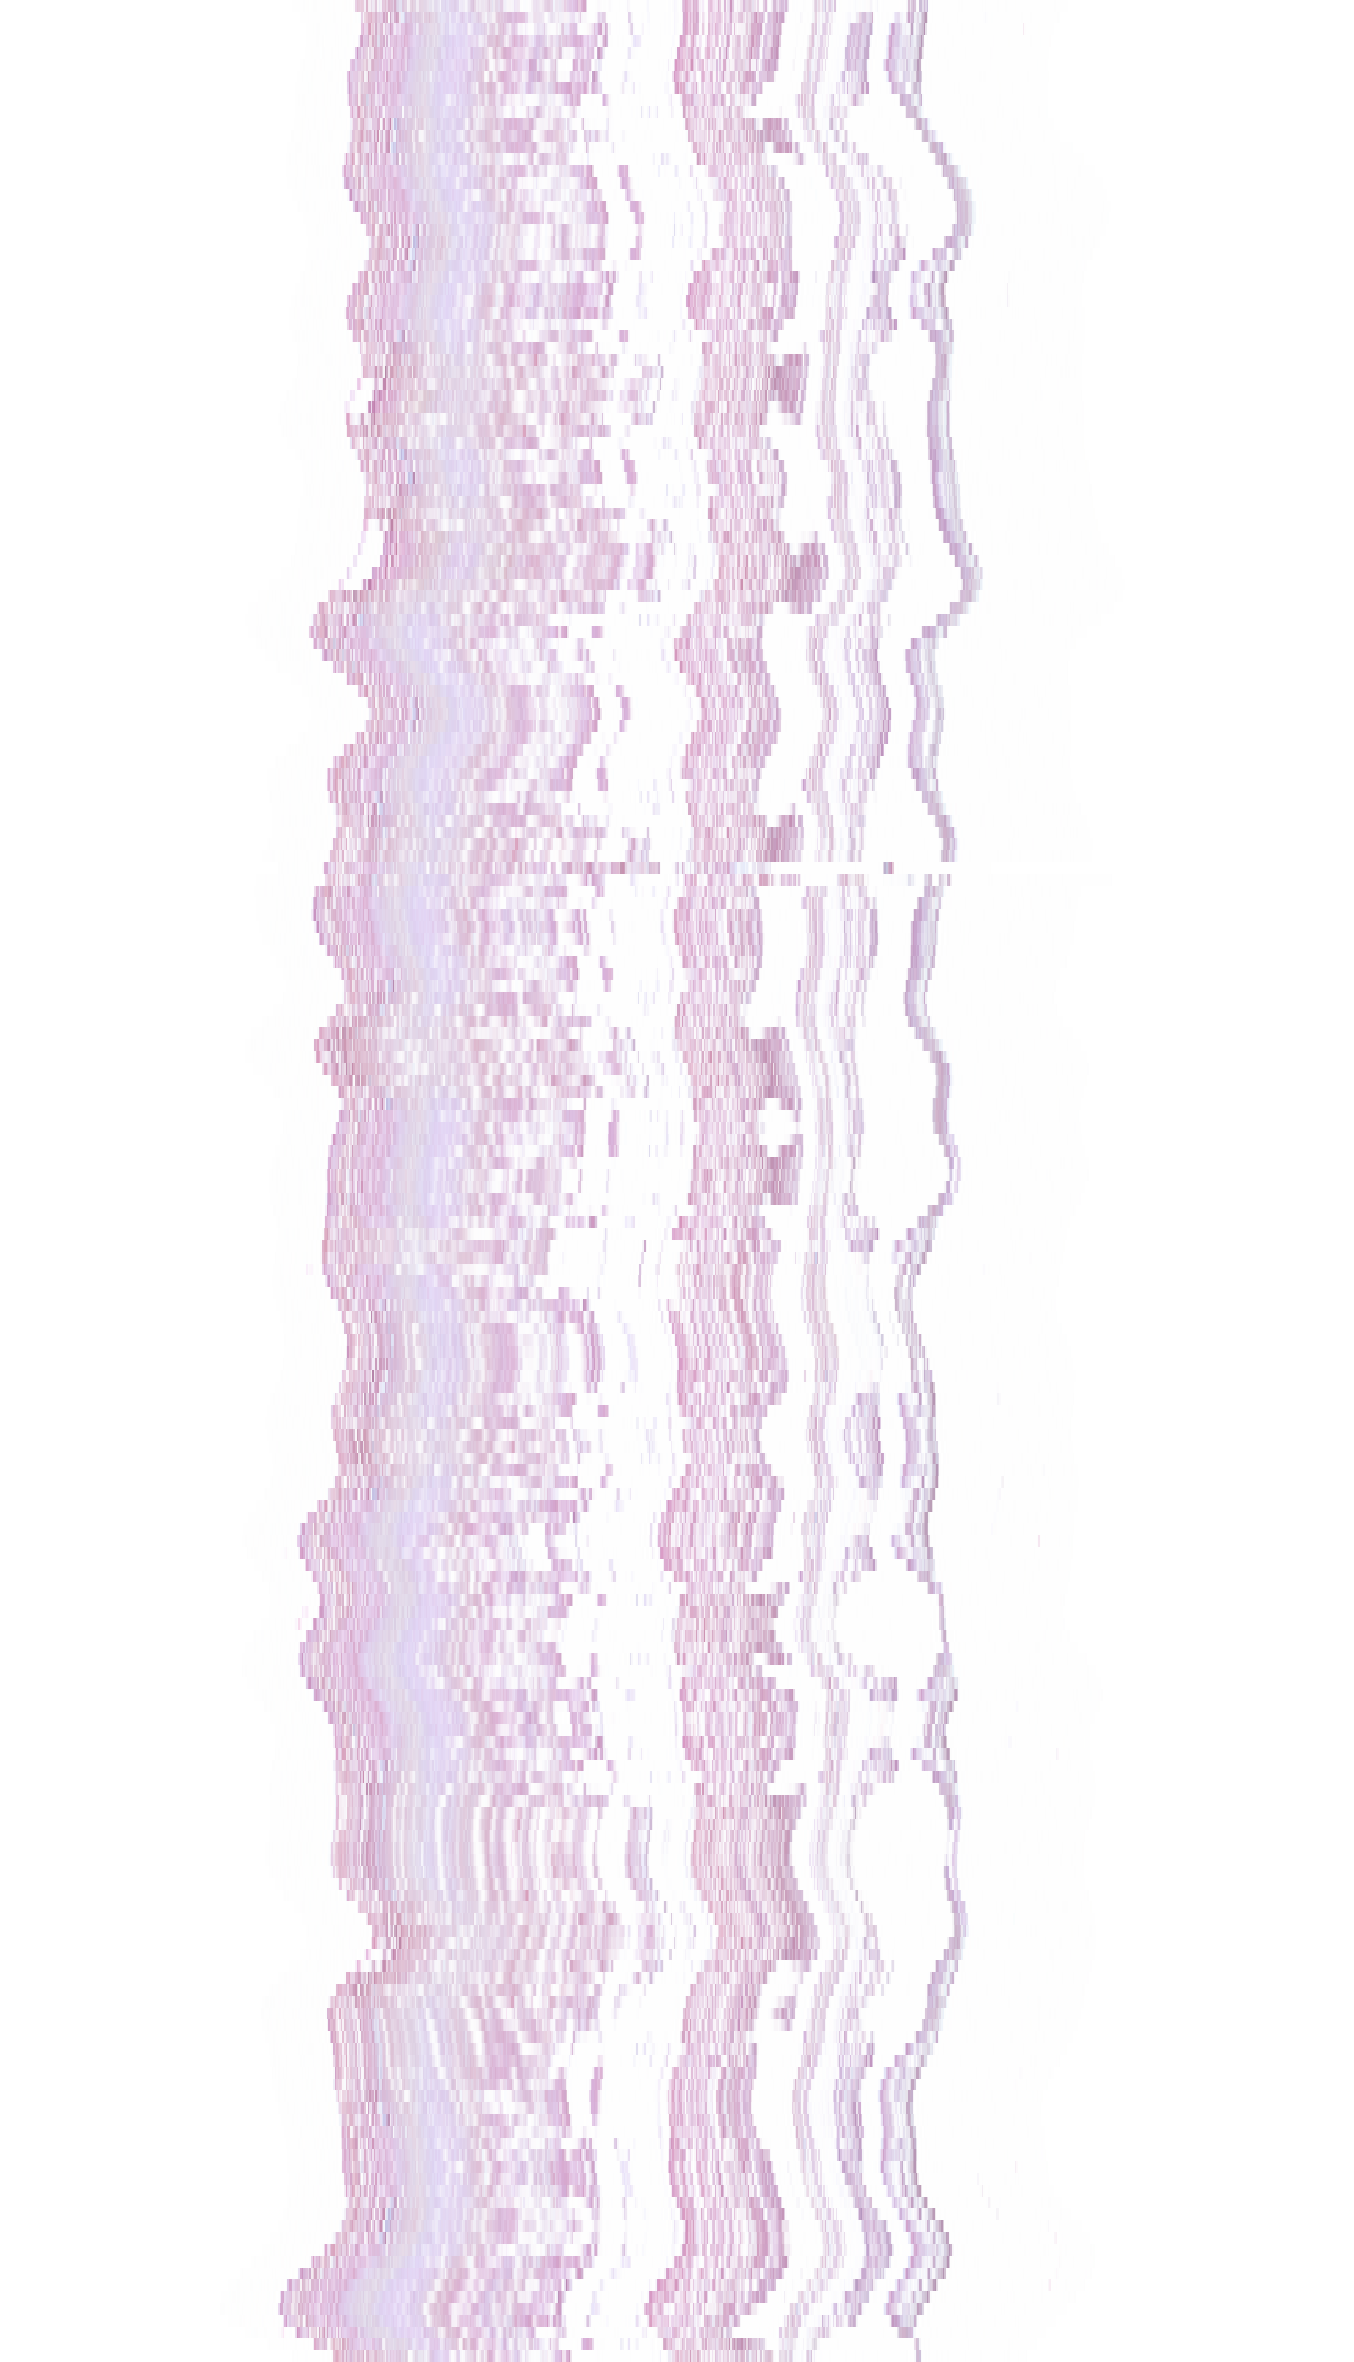
\includegraphics[height=0.4\textheight,type=pdf,ext=.pdf,read=.pdf]{Ch7/Figs/dummies/cross_section_200_alpha0.4_8_0_352}\label{fig:subfig4}}
    \subfigure[][20 iterations]{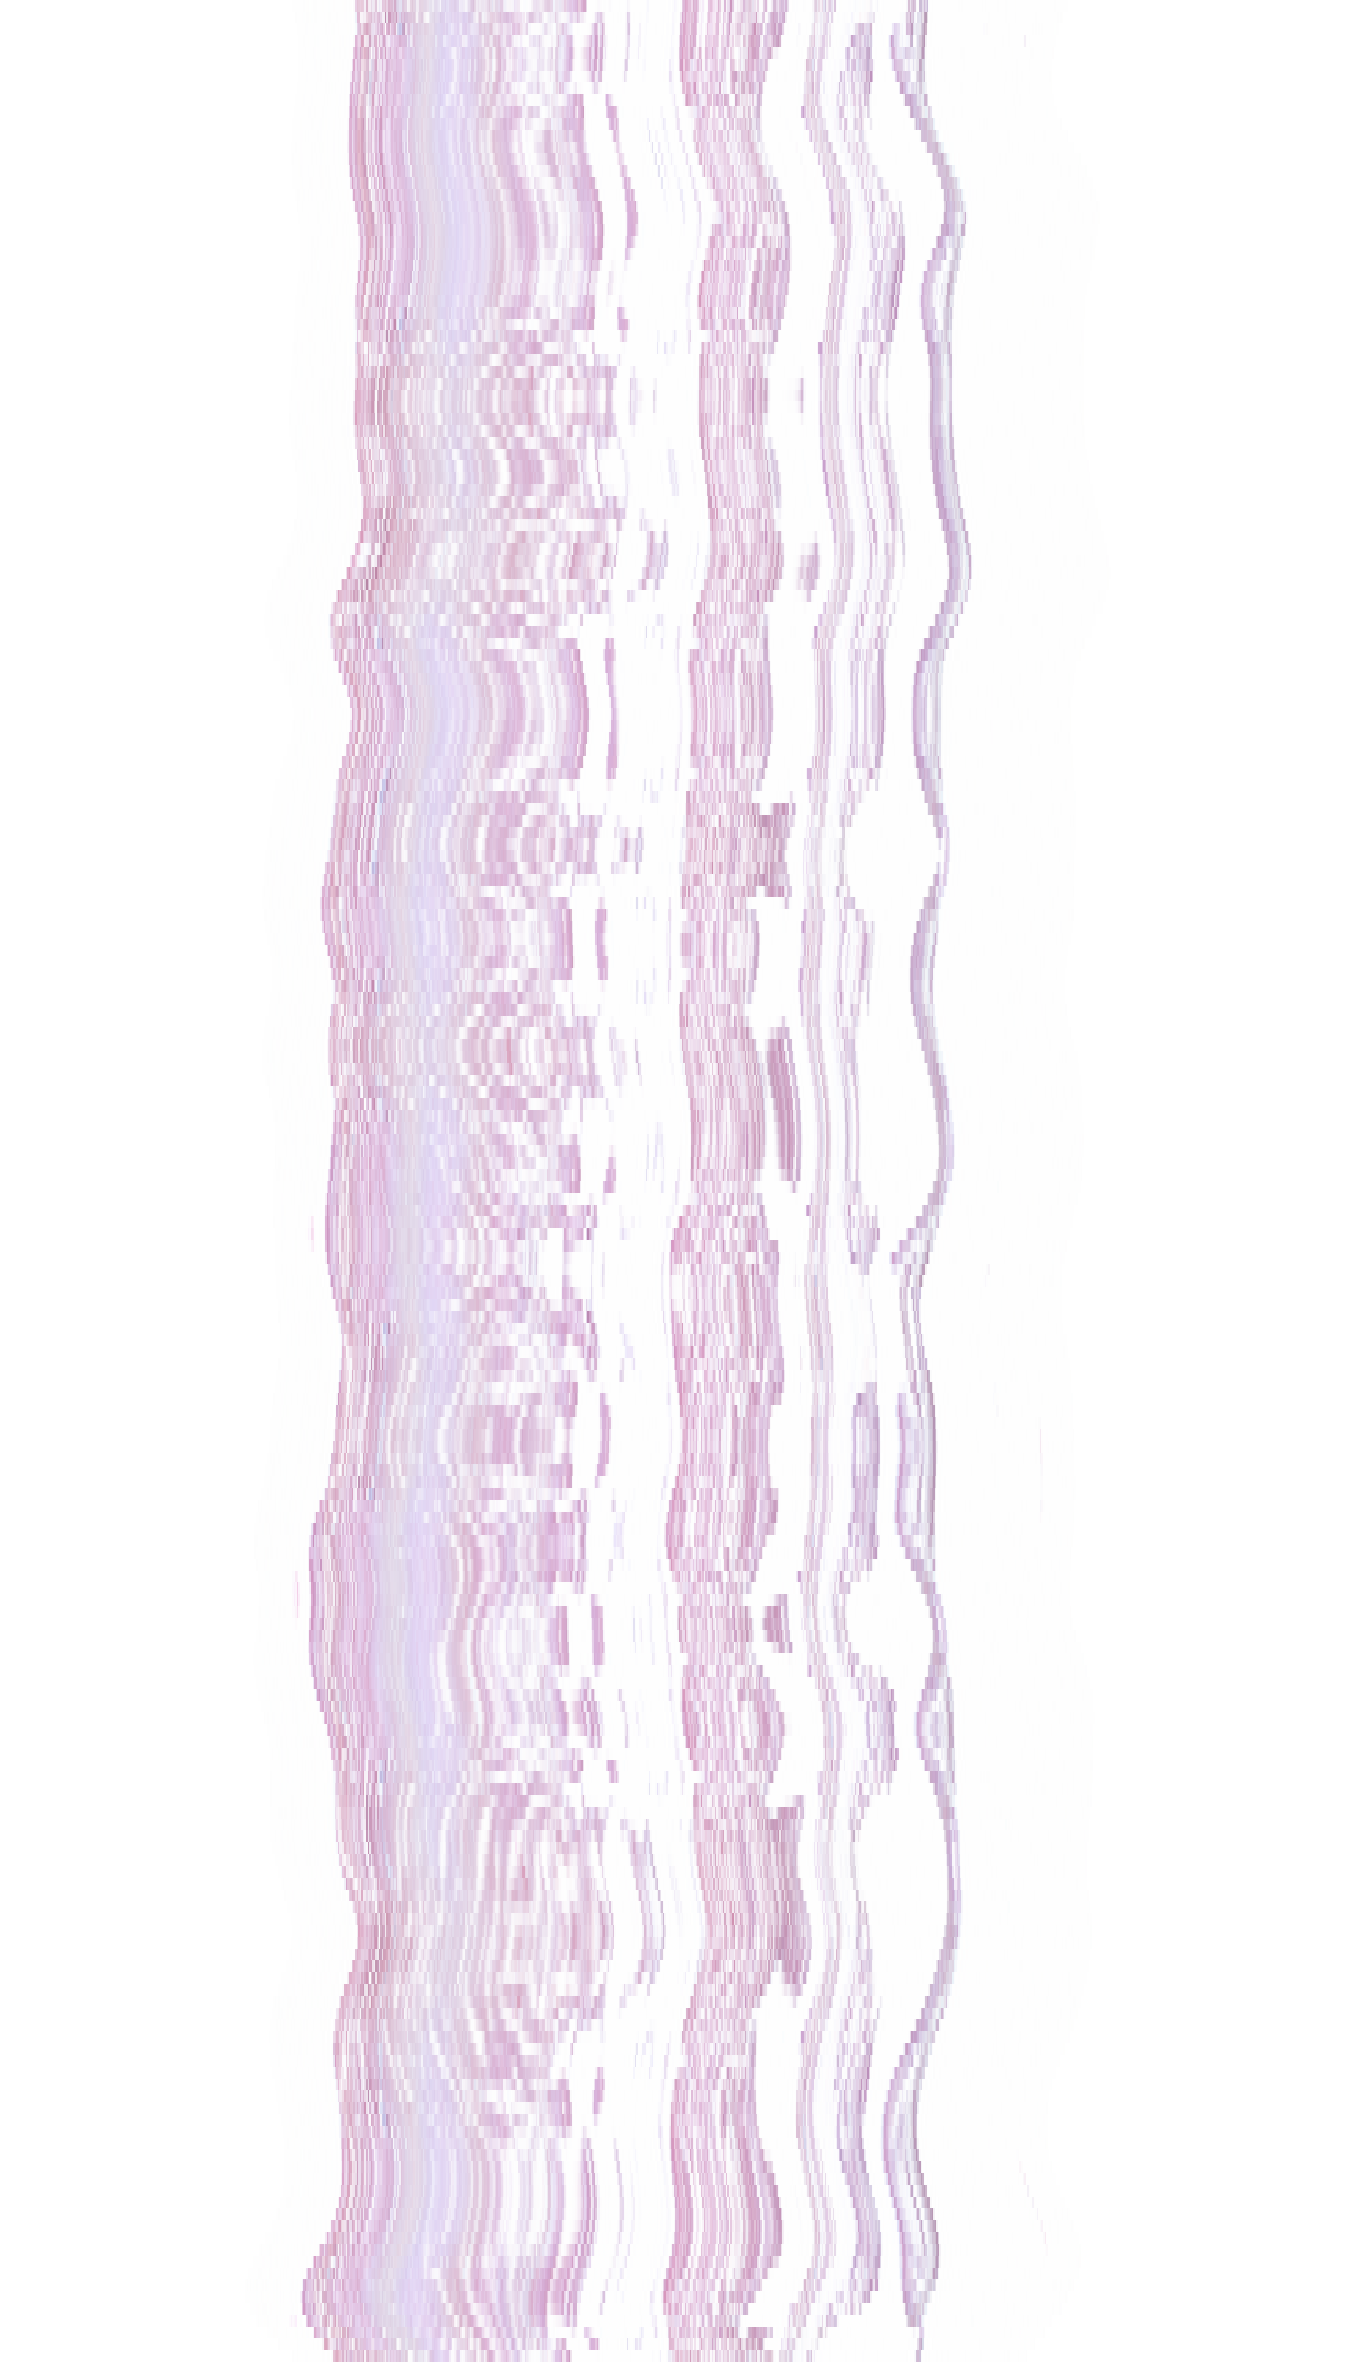
\includegraphics[height=0.4\textheight,type=pdf,ext=.pdf,read=.pdf]{Ch7/Figs/dummies/cross_section_200_alpha0.4_20_0_352}\label{fig:subfig4}}
    % filename format: cross_section_perfect_200_alpha0.4_DIMENSION_SLICE
    \subfigure[][without noise]{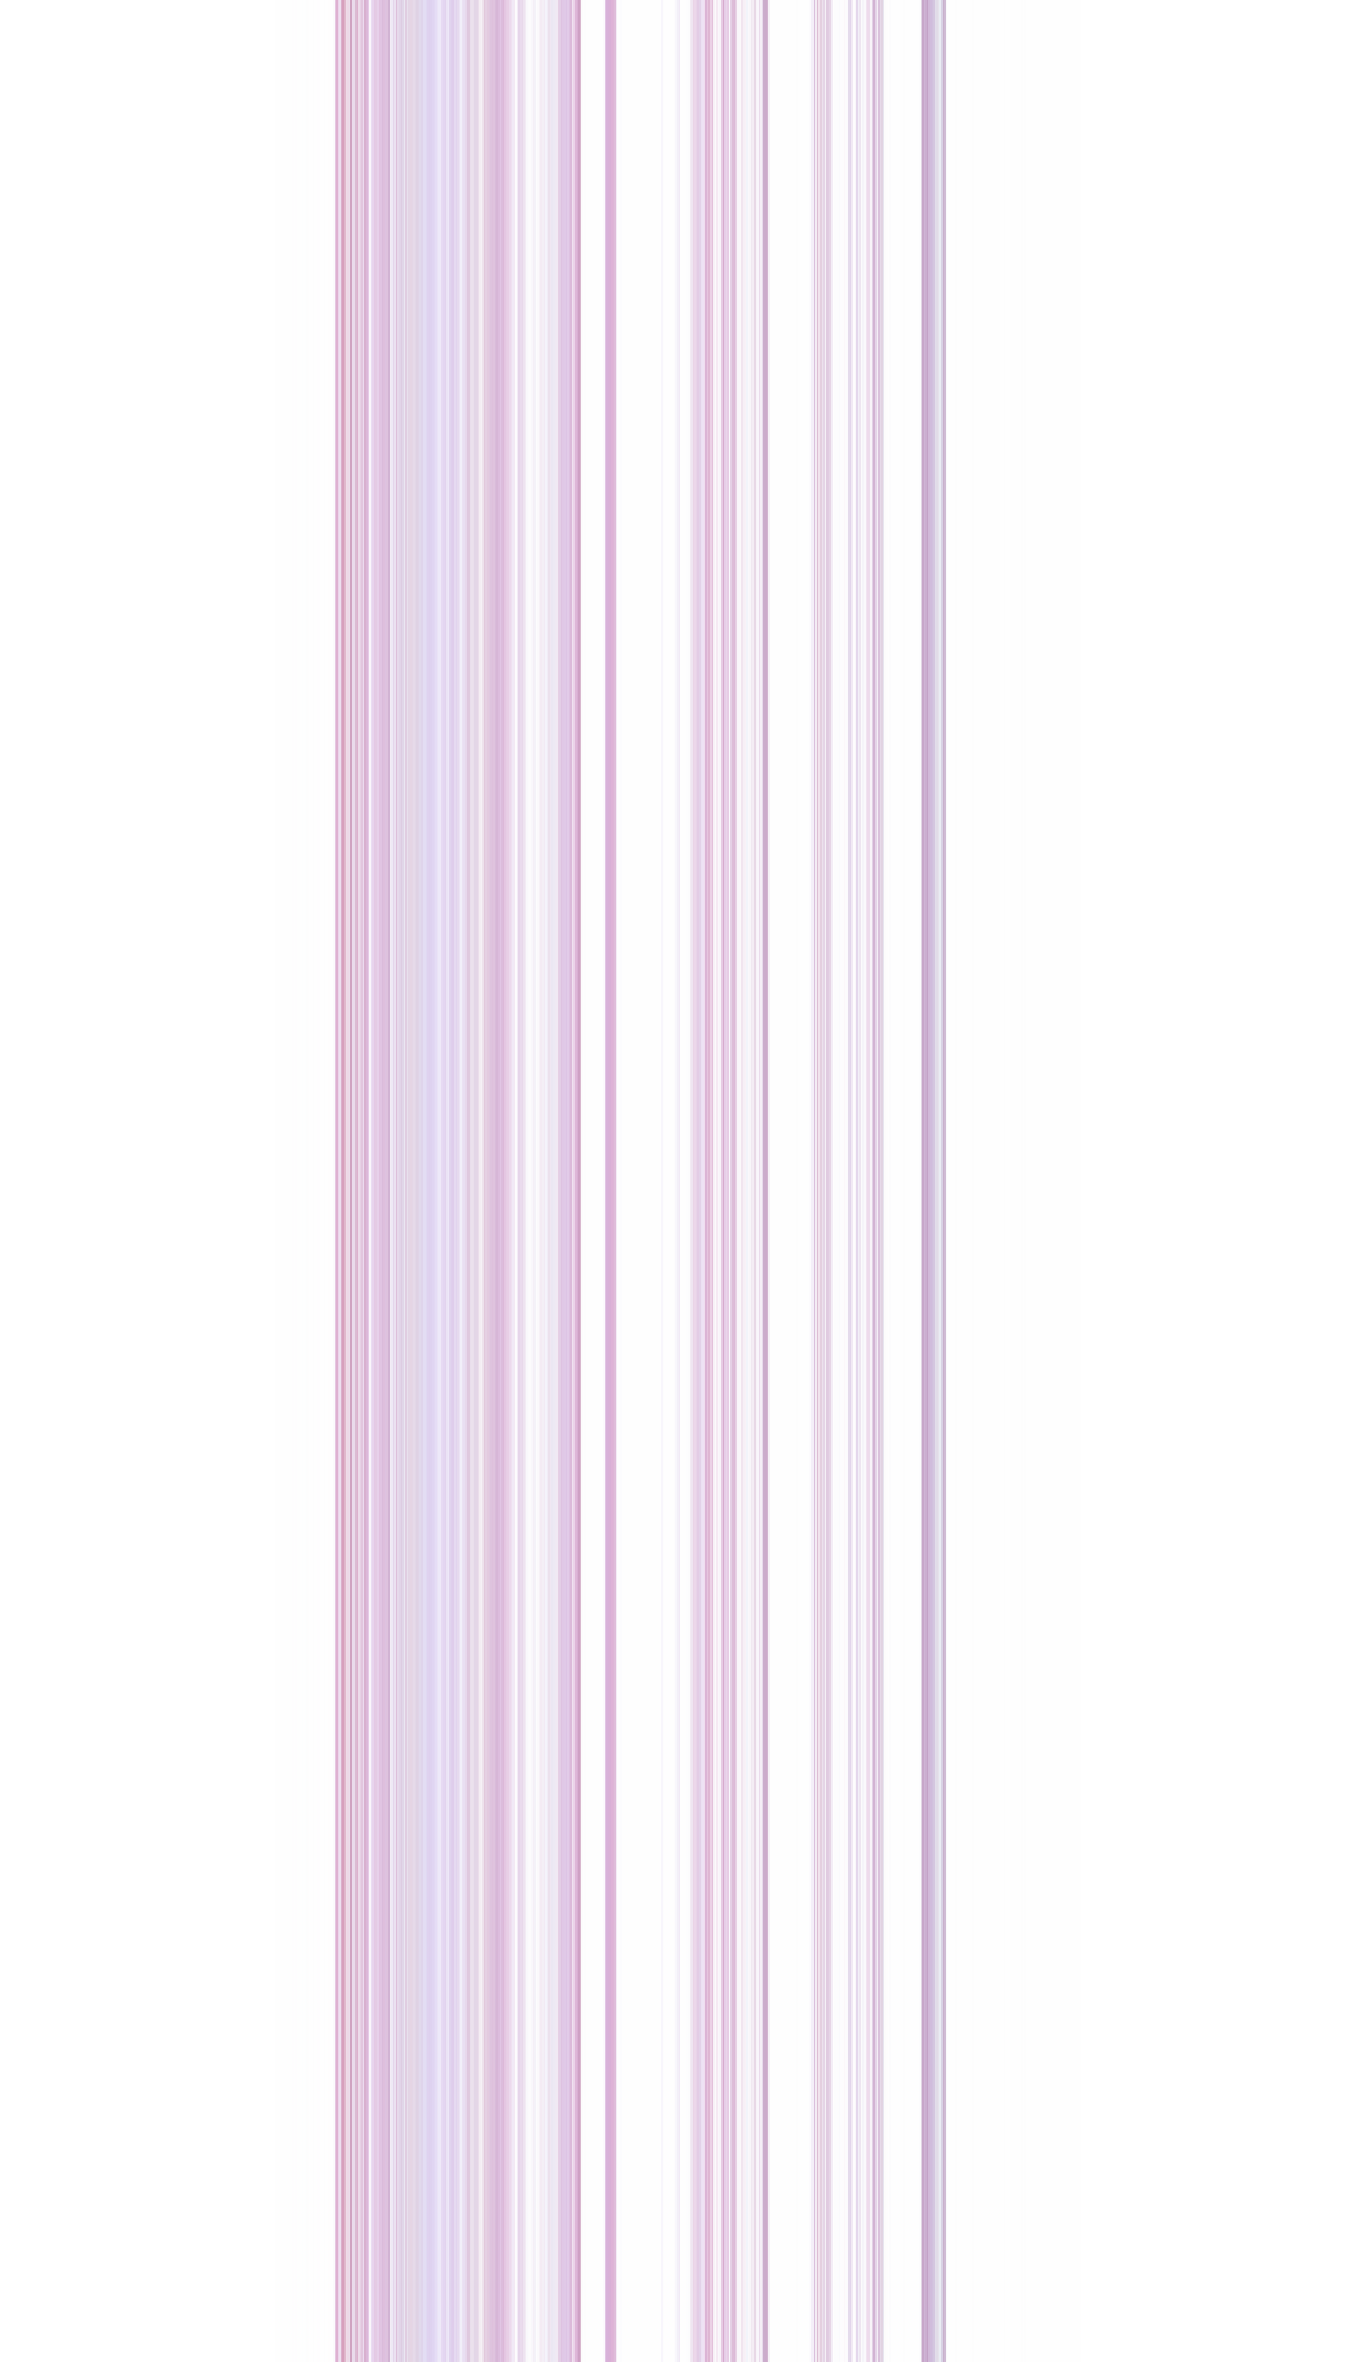
\includegraphics[height=0.4\textheight,type=pdf,ext=.pdf,read=.pdf]{Ch7/Figs/dummies/cross_section_perfect_200_alpha0.4_0_352}}
    \caption{What a nice figure! Caption of subfigures \subref{fig:subfig1}, \subref{fig:subfig2} and \subref{fig:subfig3}}
    \label{fig:dummy_cross_sections}
  \end{figure}
  
  \begin{figure}[htbp]
    \centering
    \subfigure[][0 iterations]{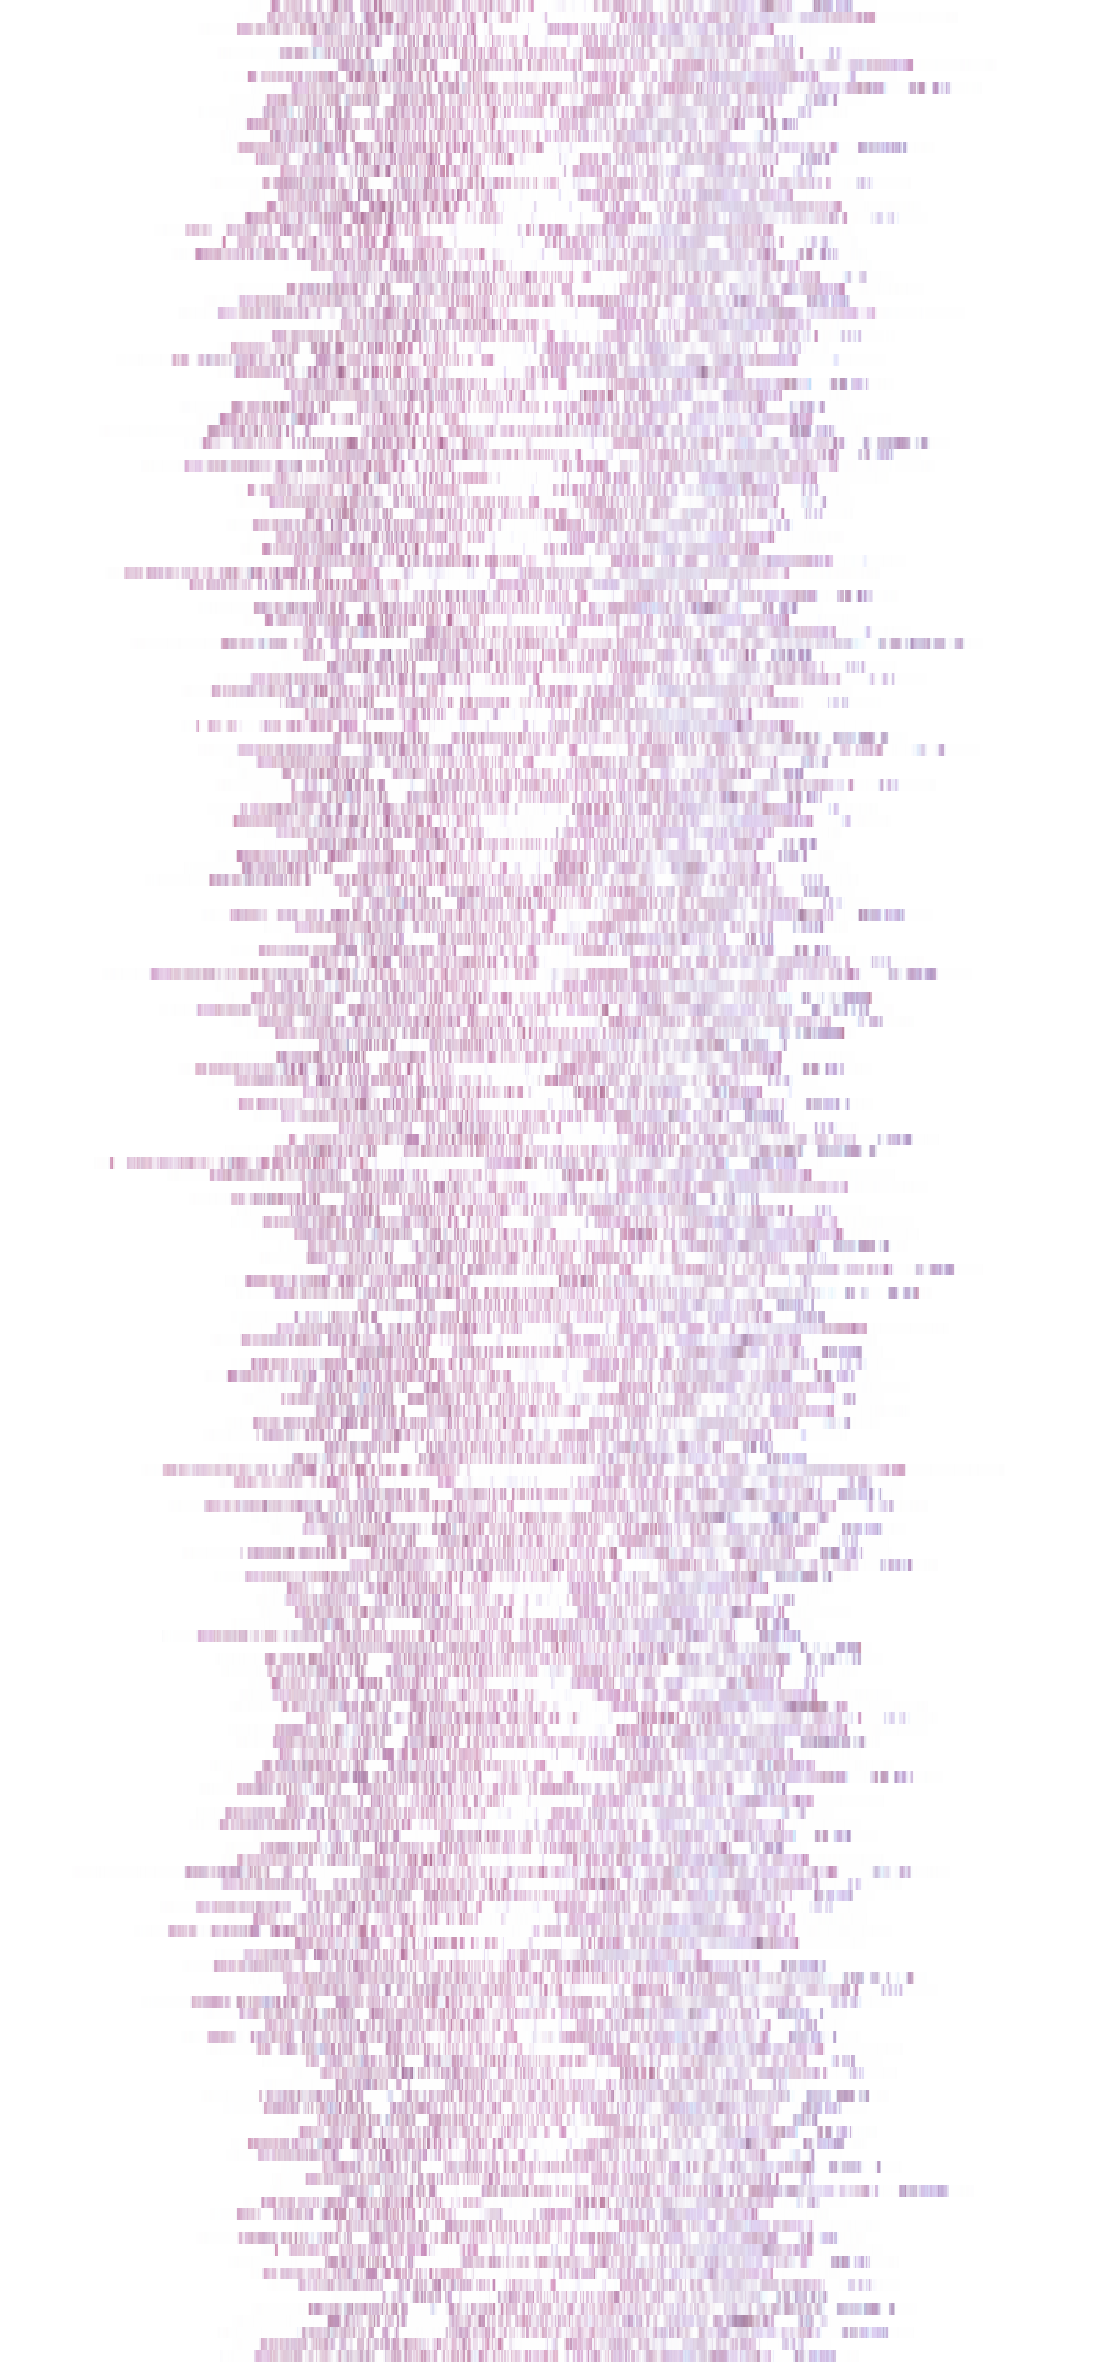
\includegraphics[height=0.4\textheight,type=pdf,ext=.pdf,read=.pdf]{Ch7/Figs/dummies/cross_section_200_alpha0.4_0_1_431}}
    \subfigure[][1 iteration]{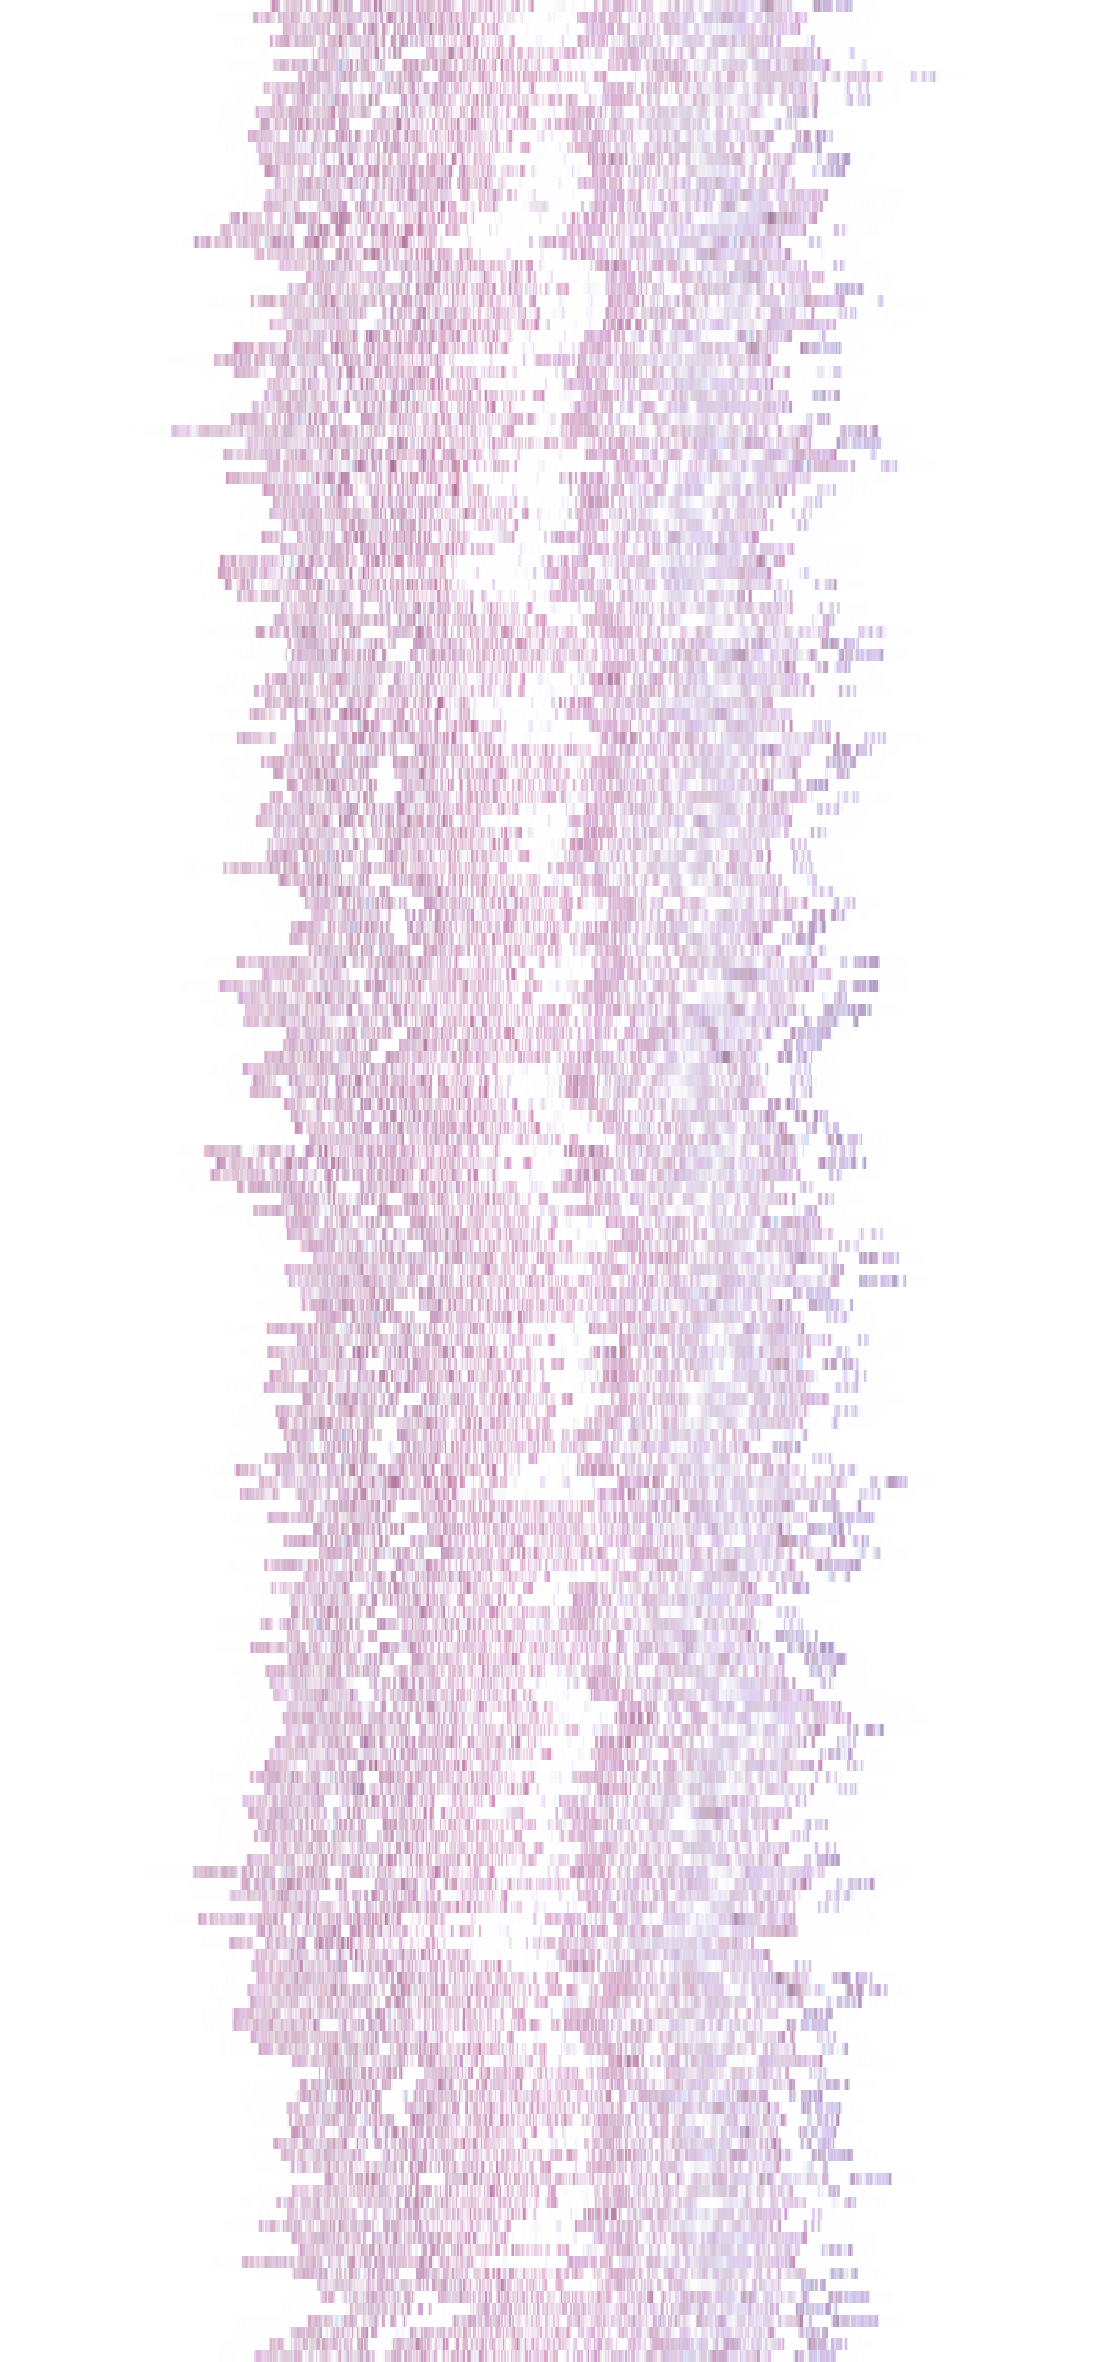
\includegraphics[height=0.4\textheight,type=pdf,ext=.pdf,read=.pdf]{Ch7/Figs/dummies/cross_section_200_alpha0.4_1_1_431}}
    \subfigure[][3 iterations]{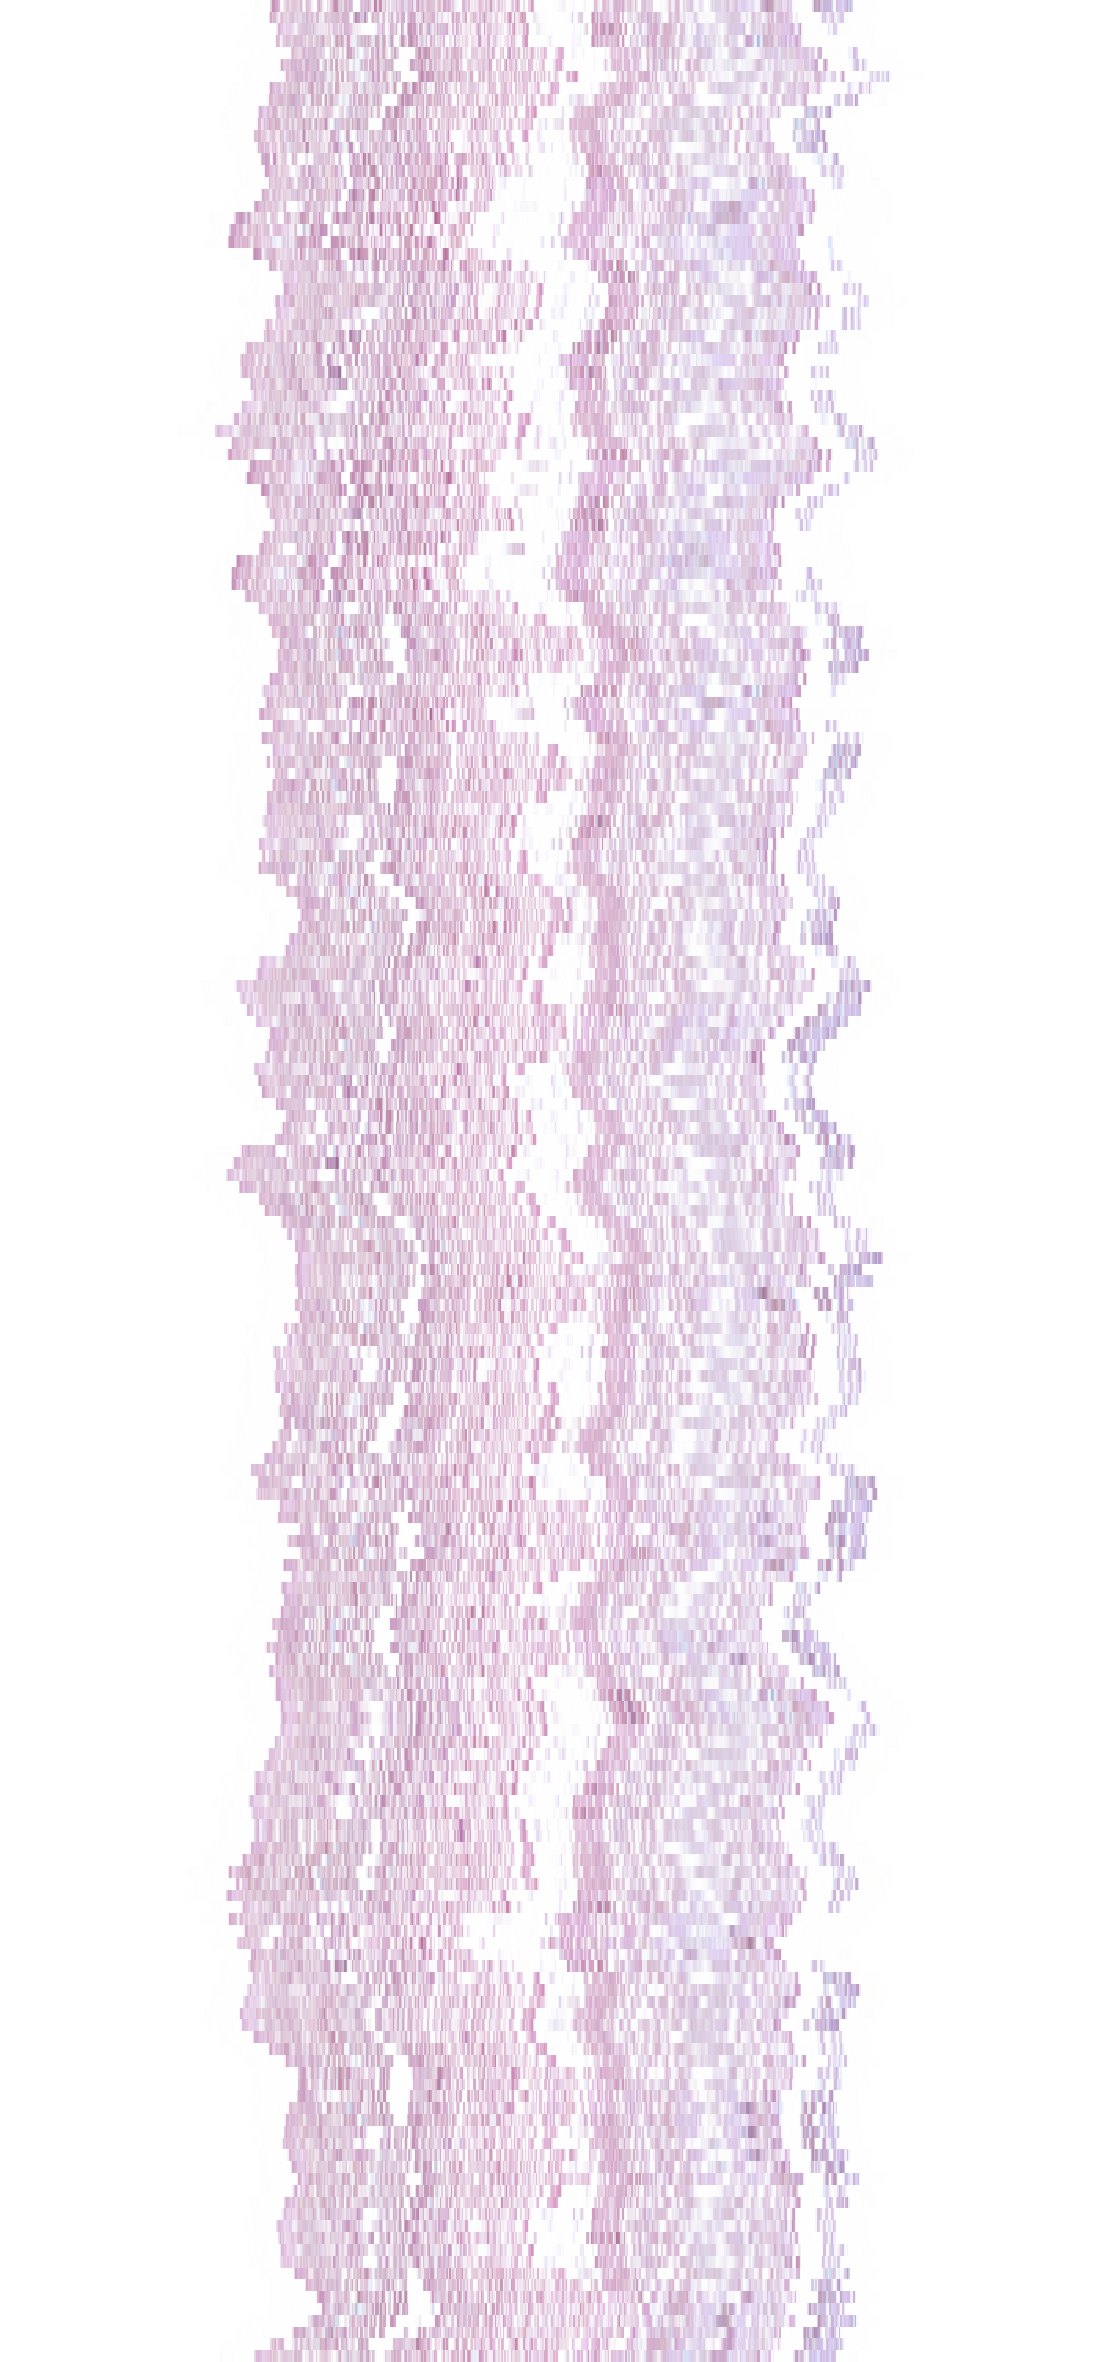
\includegraphics[height=0.4\textheight,type=pdf,ext=.pdf,read=.pdf]{Ch7/Figs/dummies/cross_section_200_alpha0.4_3_1_431}}
    \subfigure[][8 iterations]{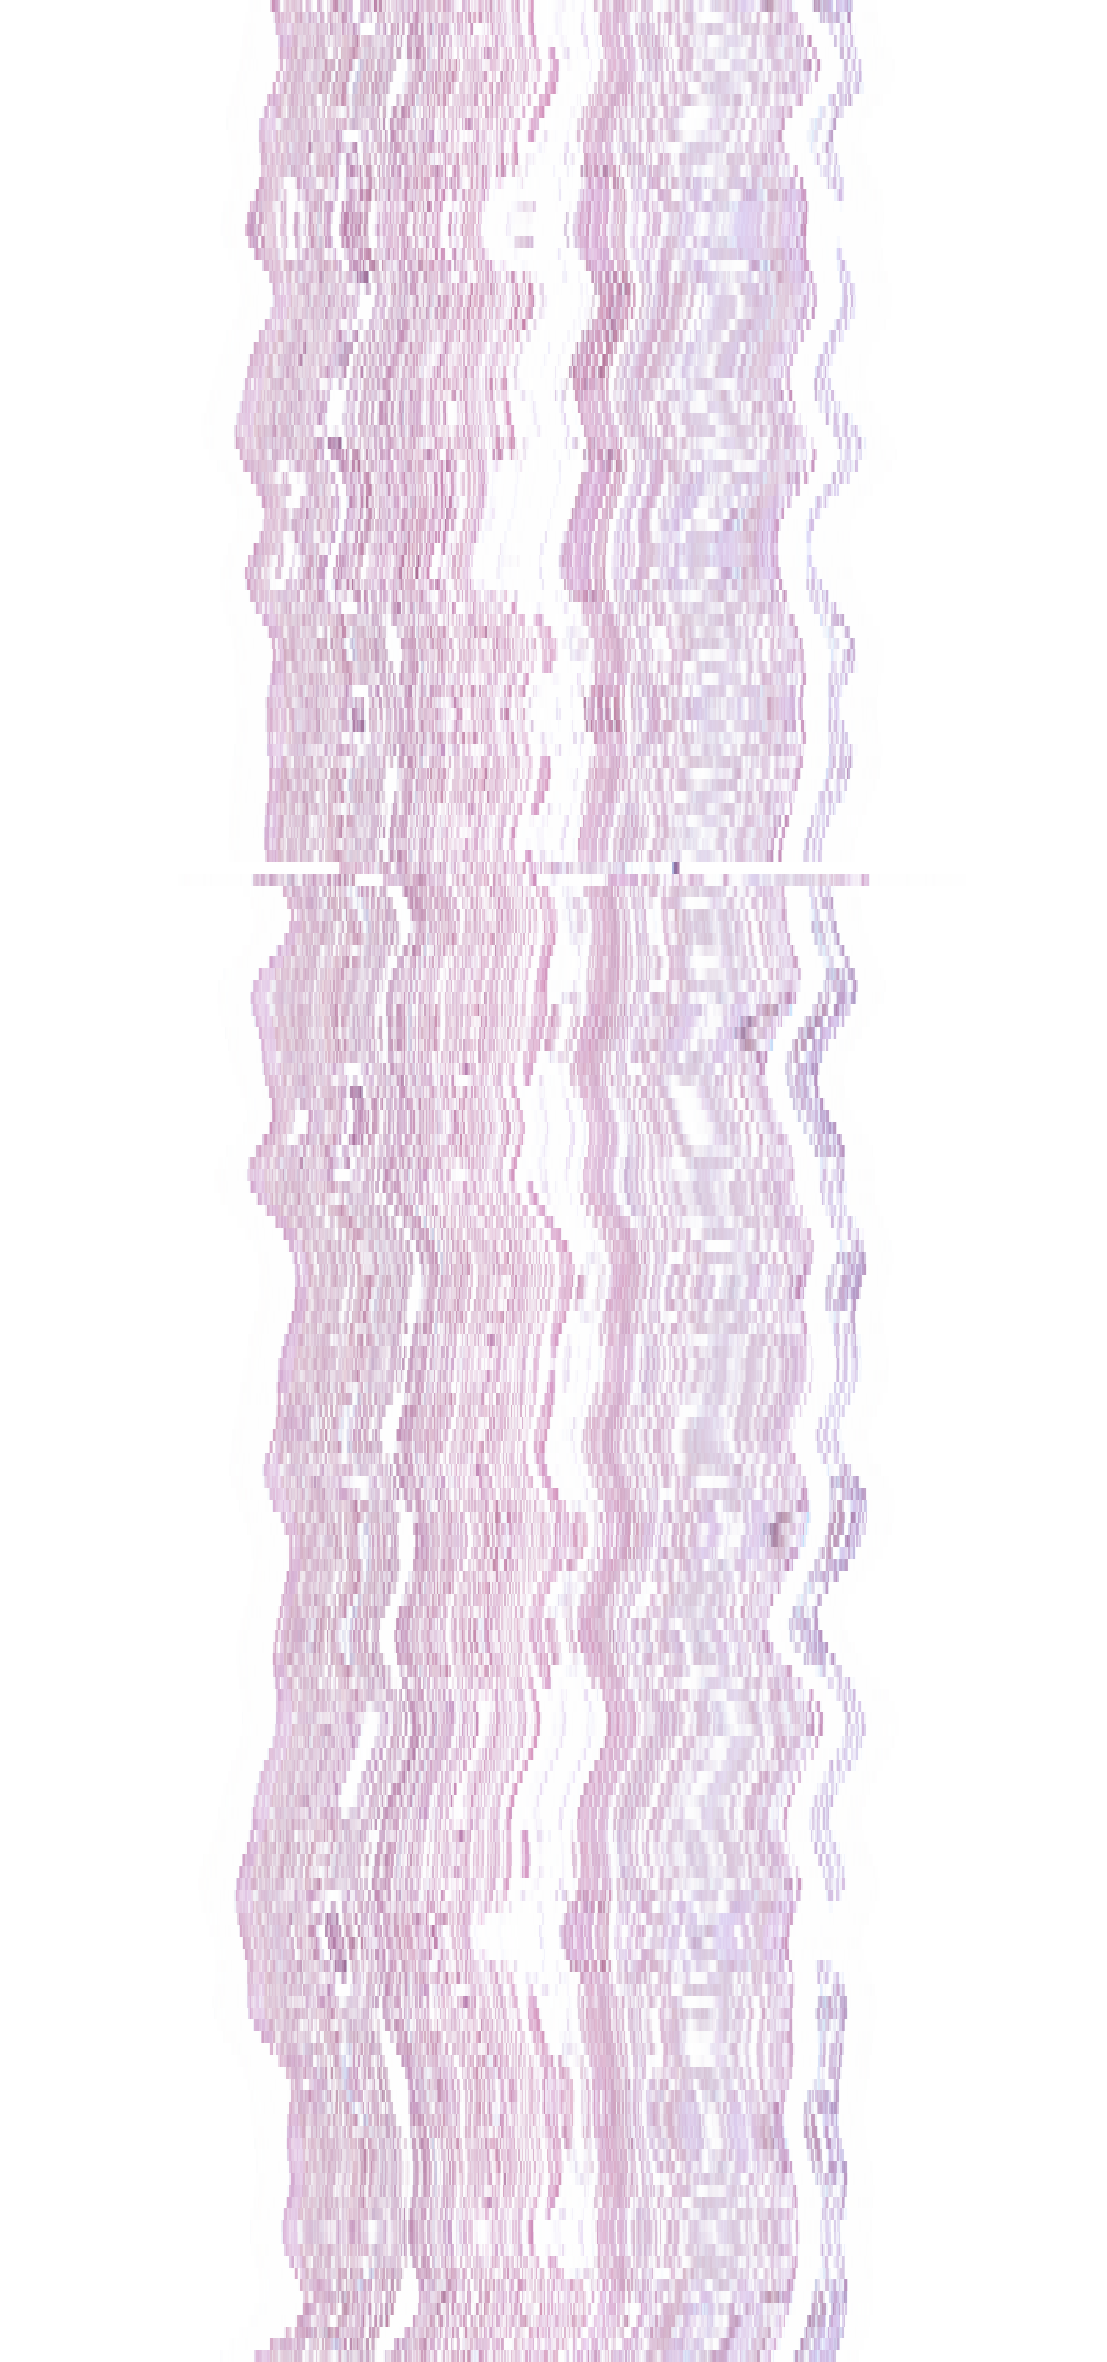
\includegraphics[height=0.4\textheight,type=pdf,ext=.pdf,read=.pdf]{Ch7/Figs/dummies/cross_section_200_alpha0.4_8_1_431}}
    \subfigure[][20 iterations]{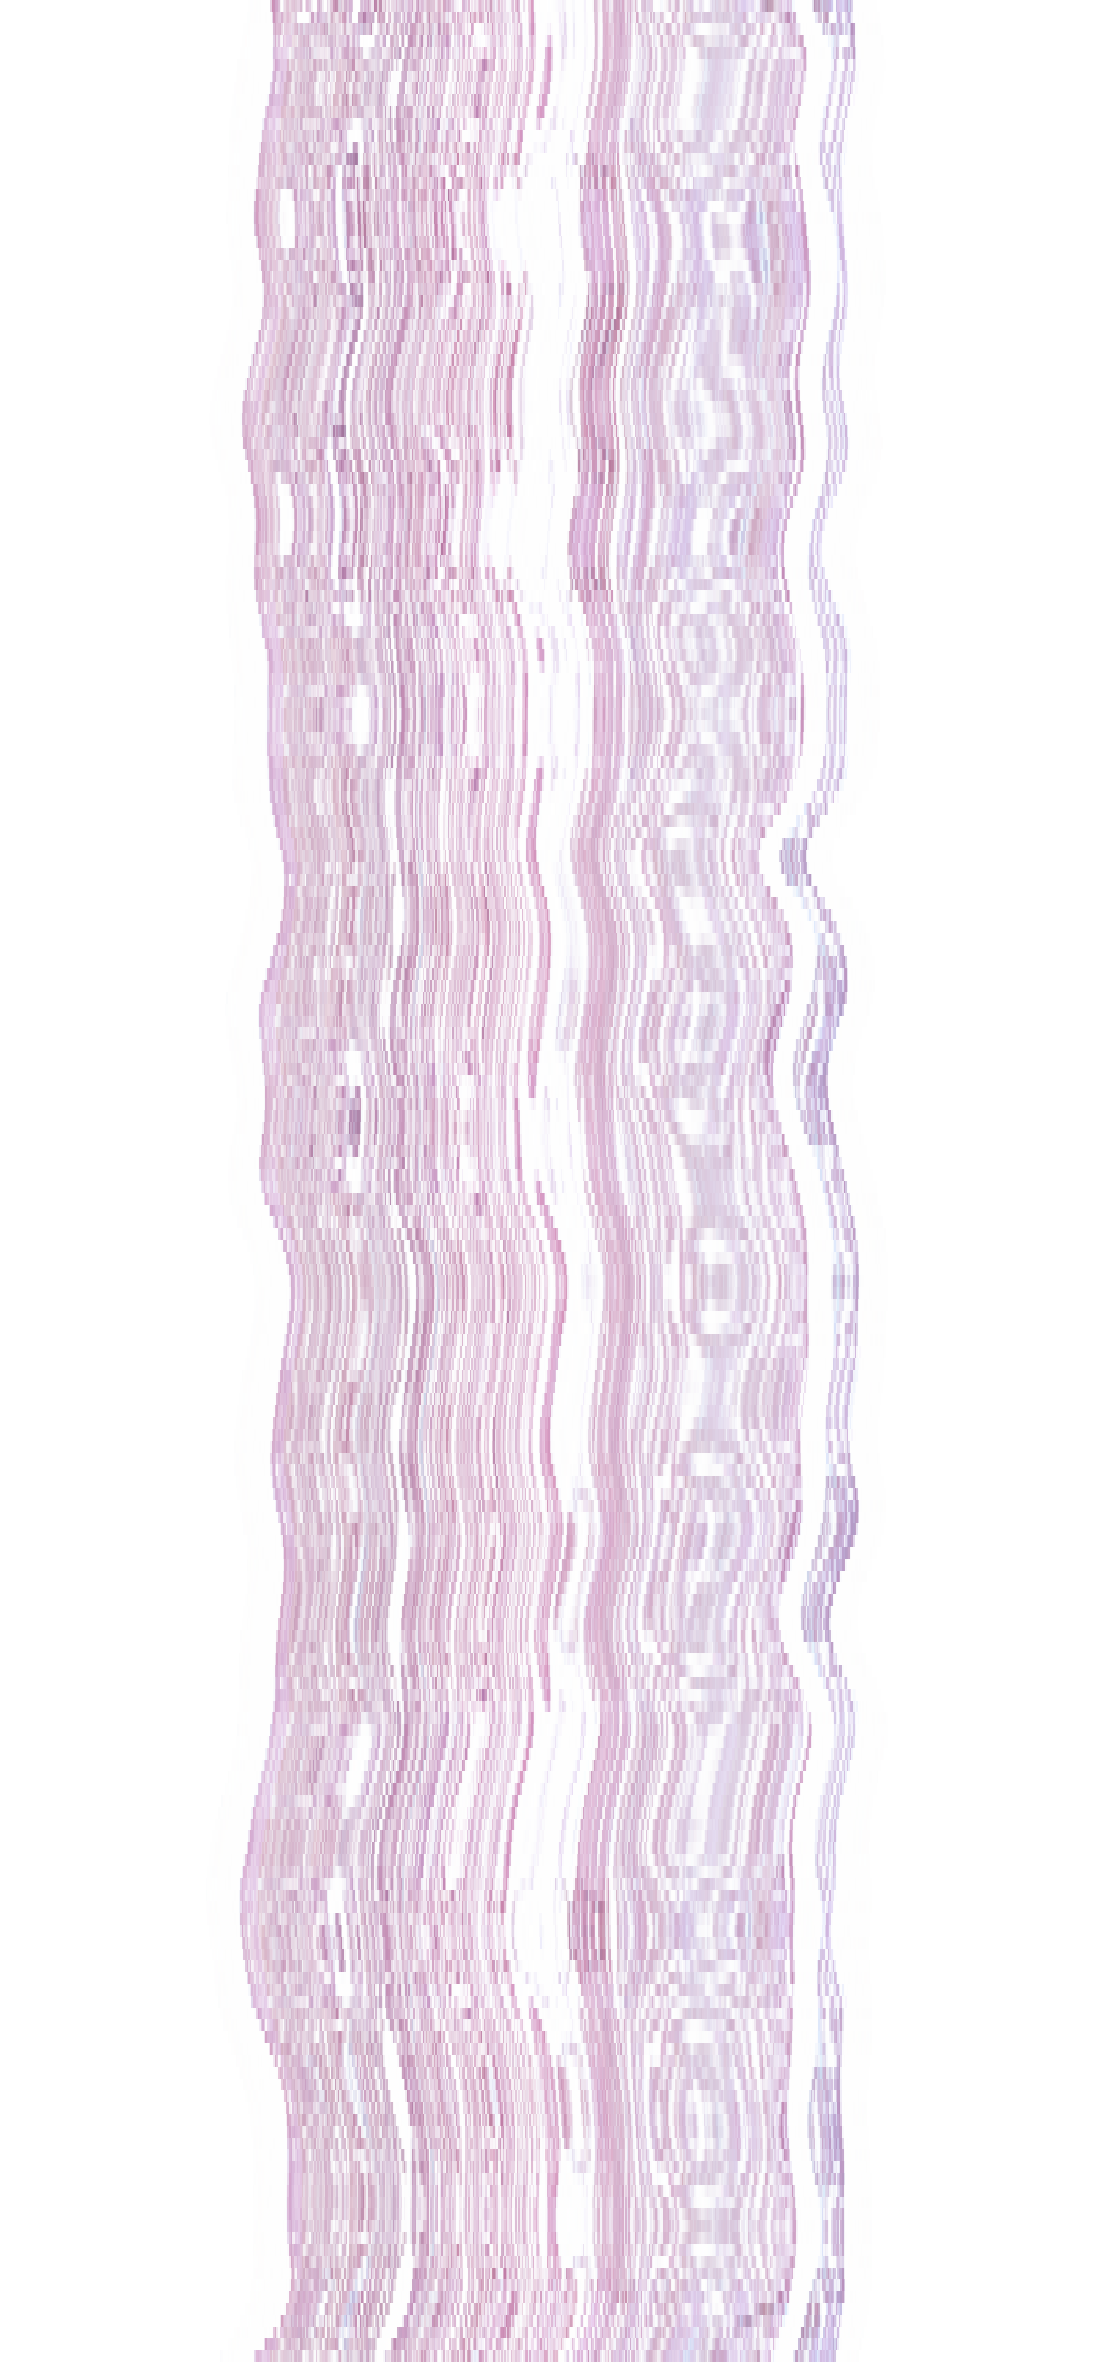
\includegraphics[height=0.4\textheight,type=pdf,ext=.pdf,read=.pdf]{Ch7/Figs/dummies/cross_section_200_alpha0.4_20_1_431}}
    \subfigure[][without noise]{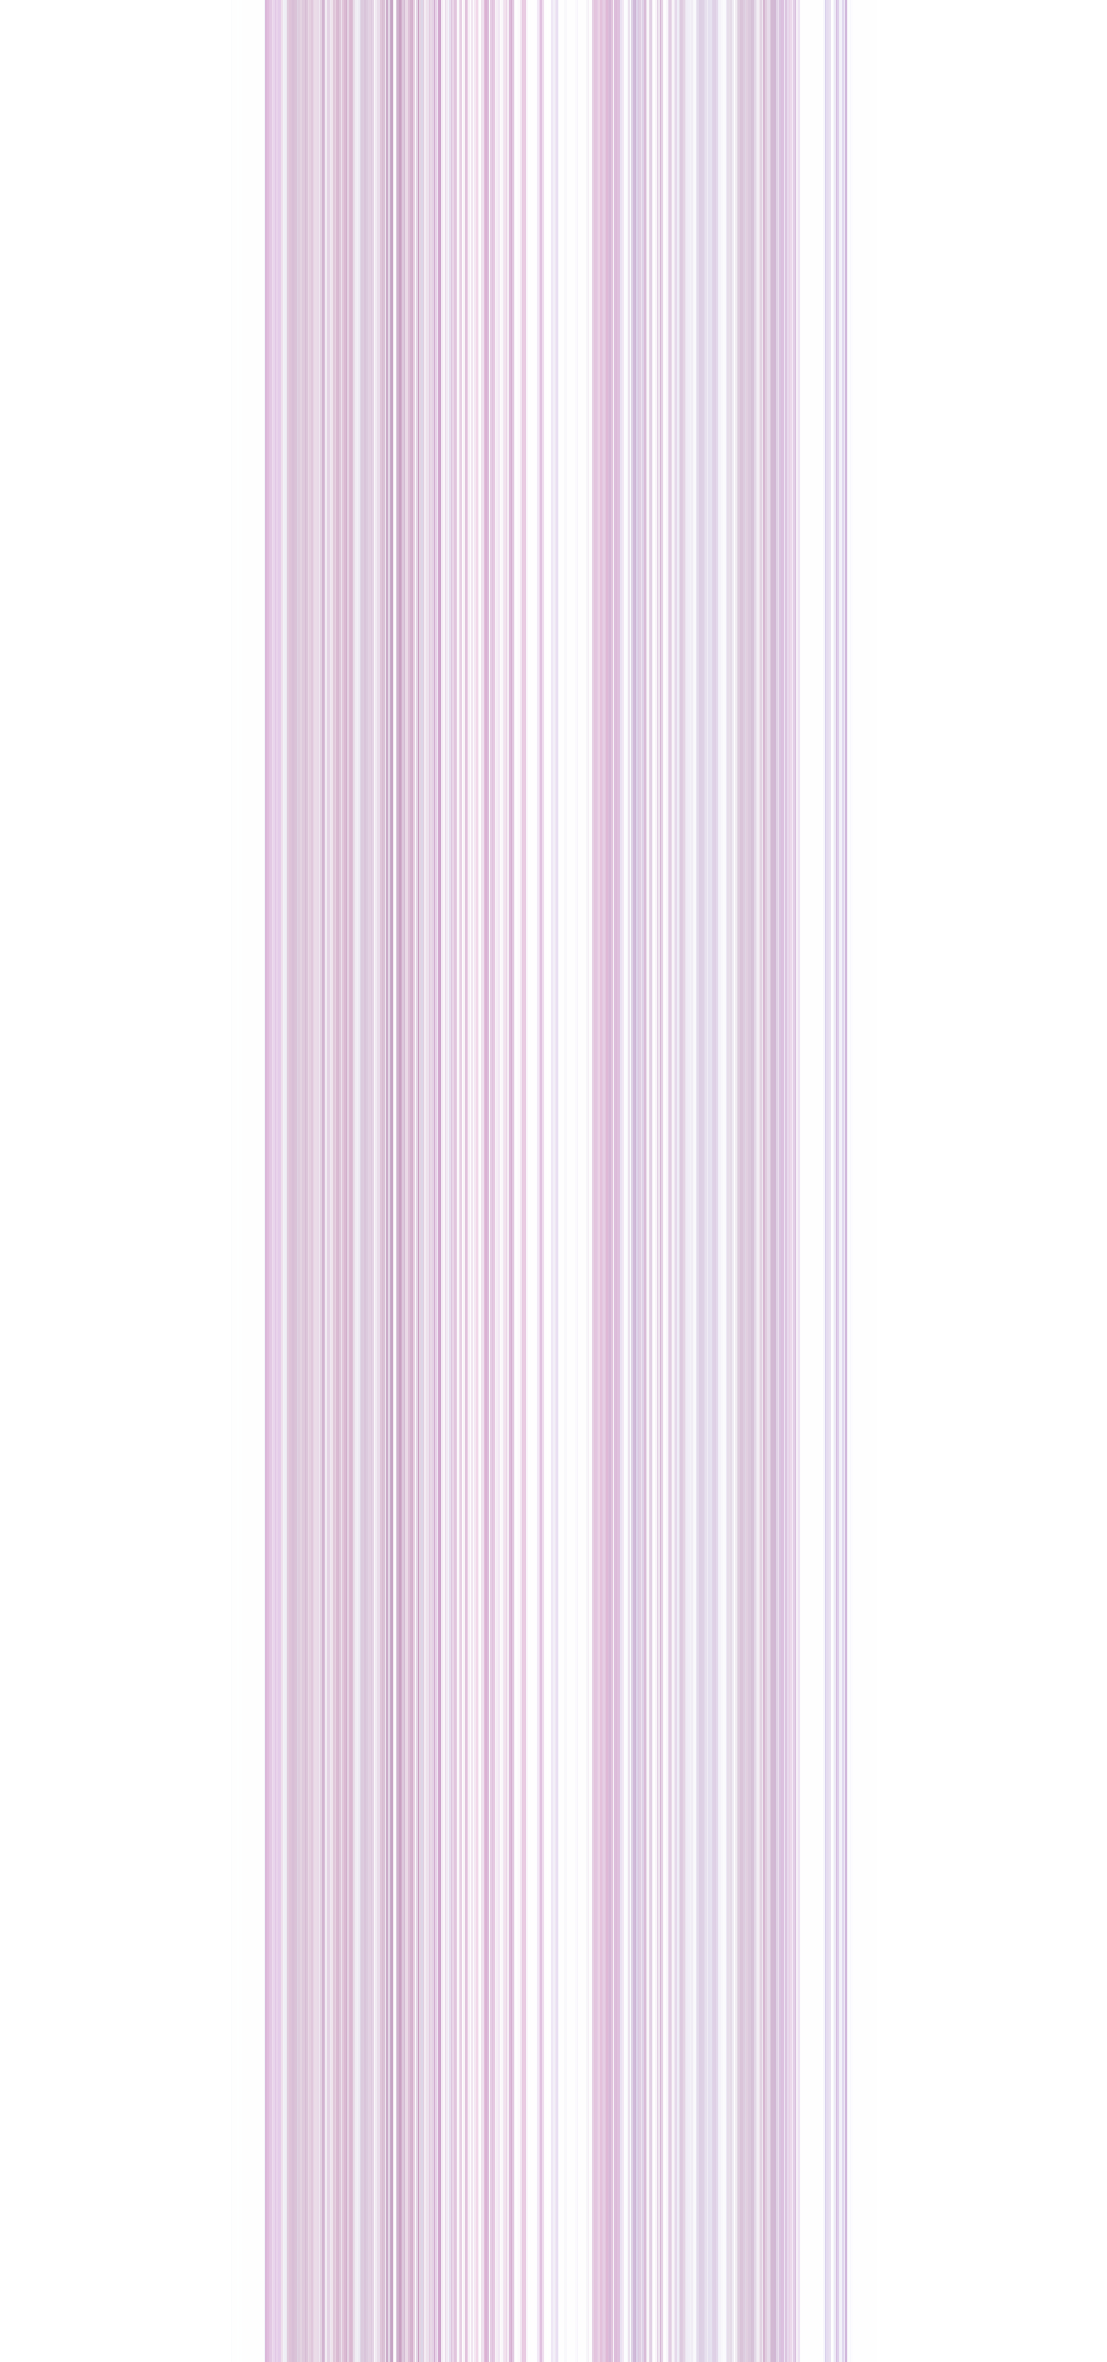
\includegraphics[height=0.4\textheight,type=pdf,ext=.pdf,read=.pdf]{Ch7/Figs/dummies/cross_section_perfect_200_alpha0.4_1_431}}
    \caption{What a nice figure!}
    \label{fig:dummy_cross_sections}
  \end{figure}
    
  % rotated
  \begin{figure}[htbp]
    \centering
    \subfigure[][0 iterations]{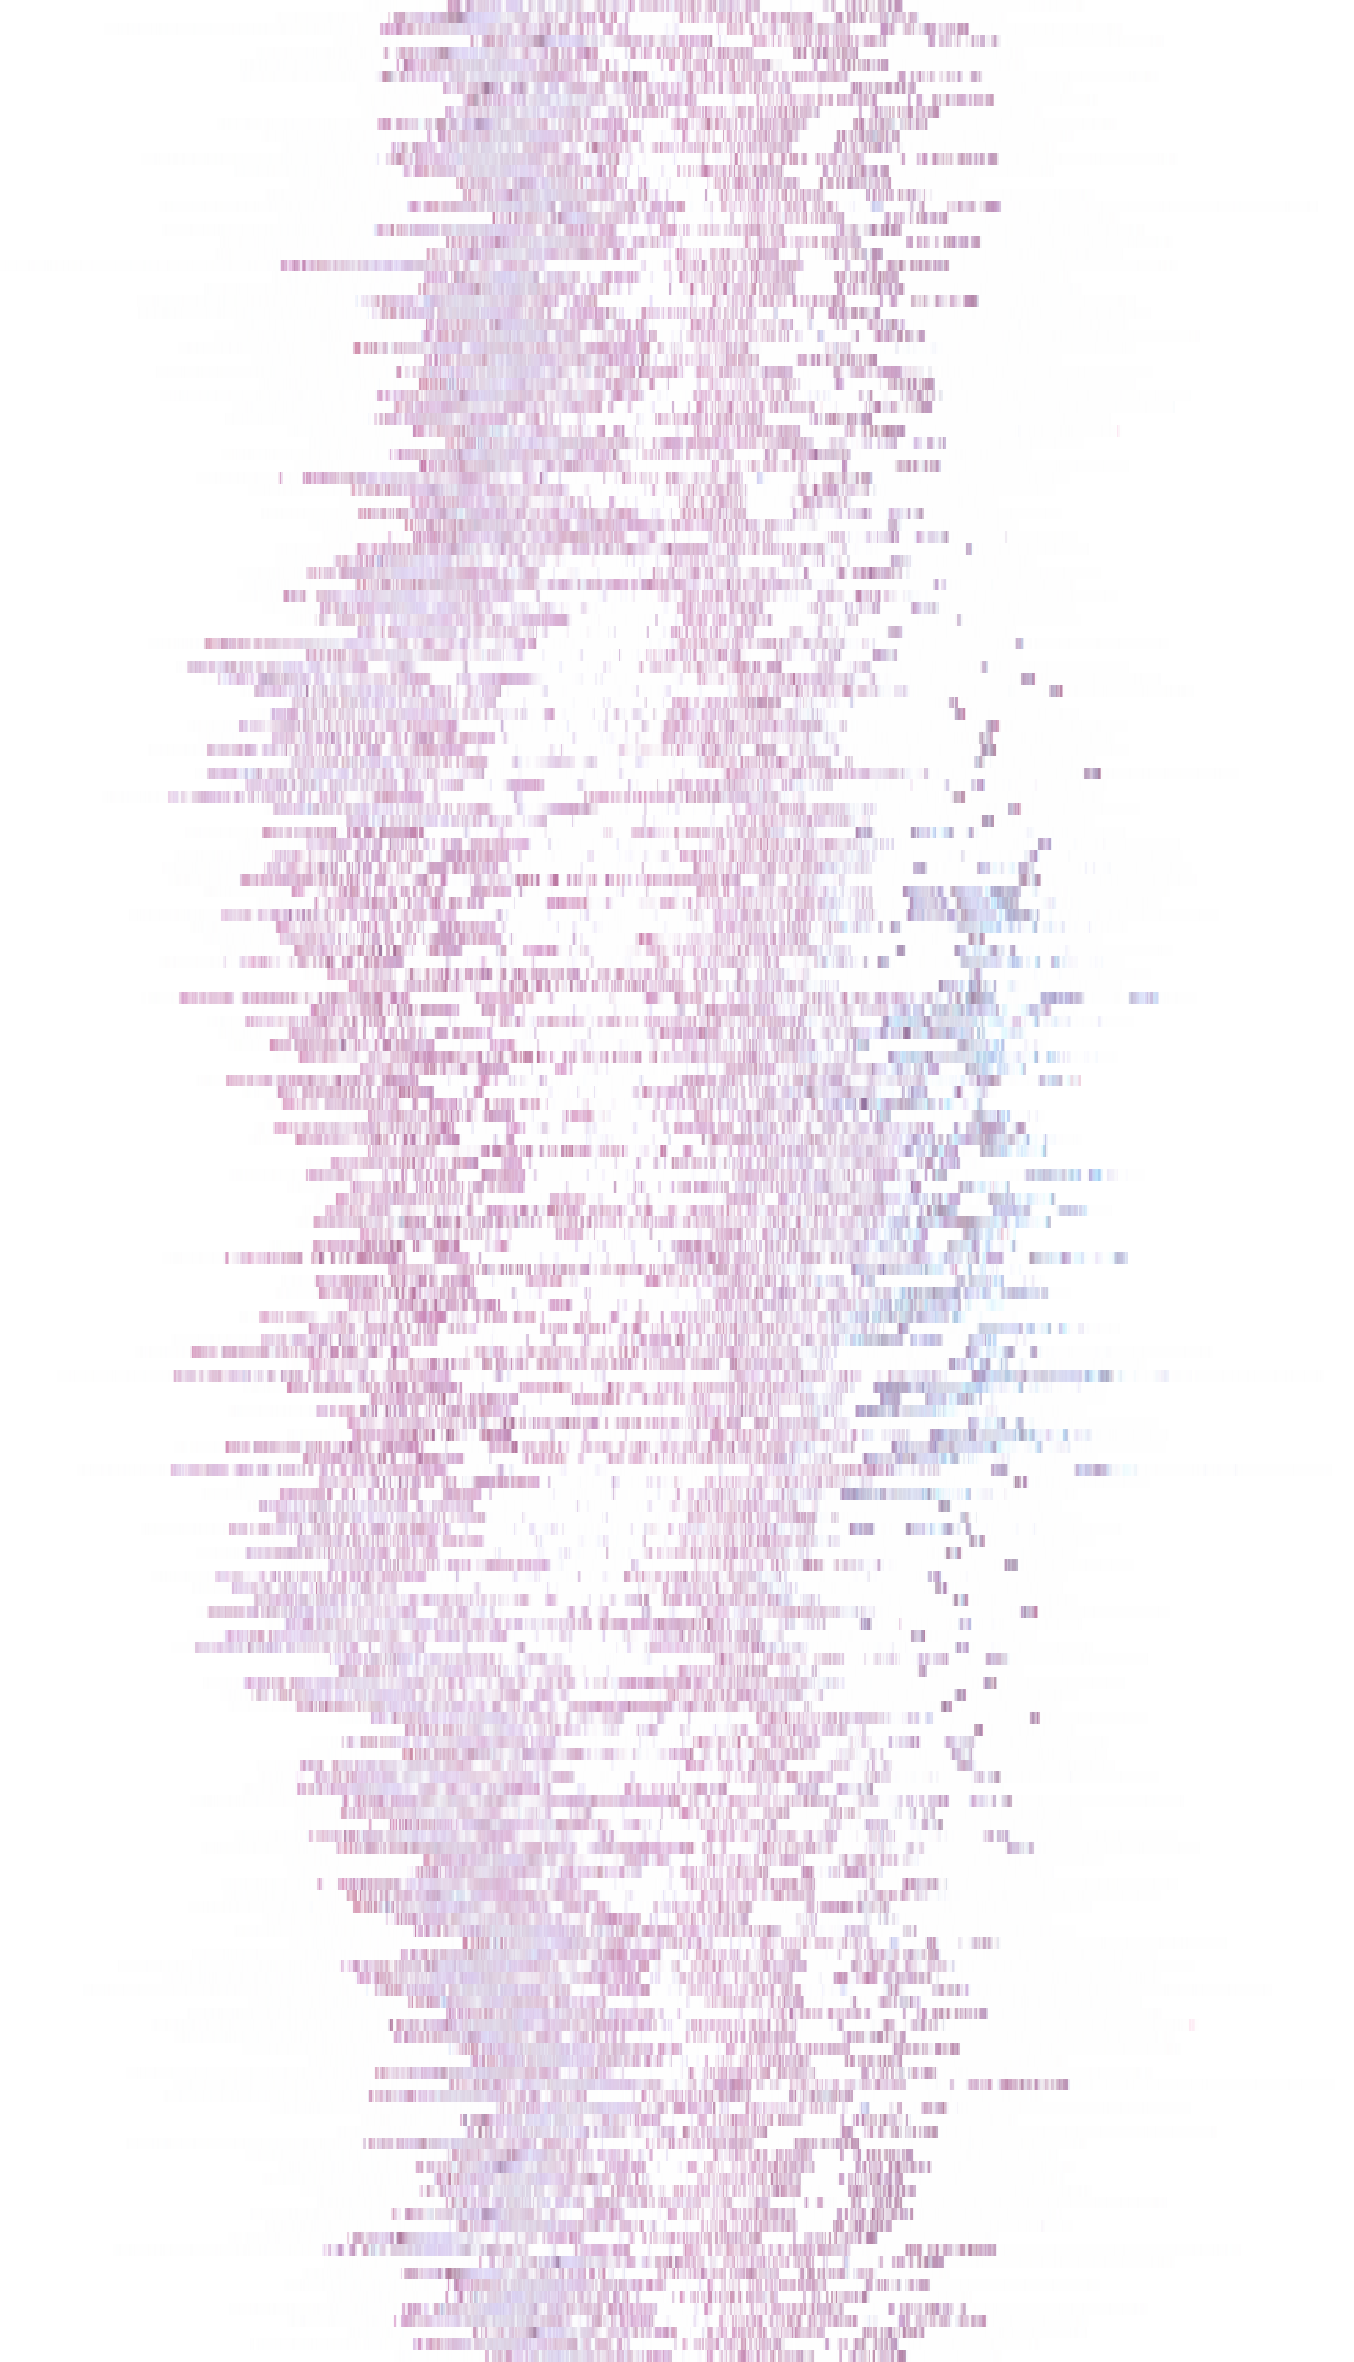
\includegraphics[height=0.4\textheight,type=pdf,ext=.pdf,read=.pdf]{Ch7/Figs/dummies/cross_section_200_alpha0.4r_0_0_352}}
    \subfigure[][1 iteration]{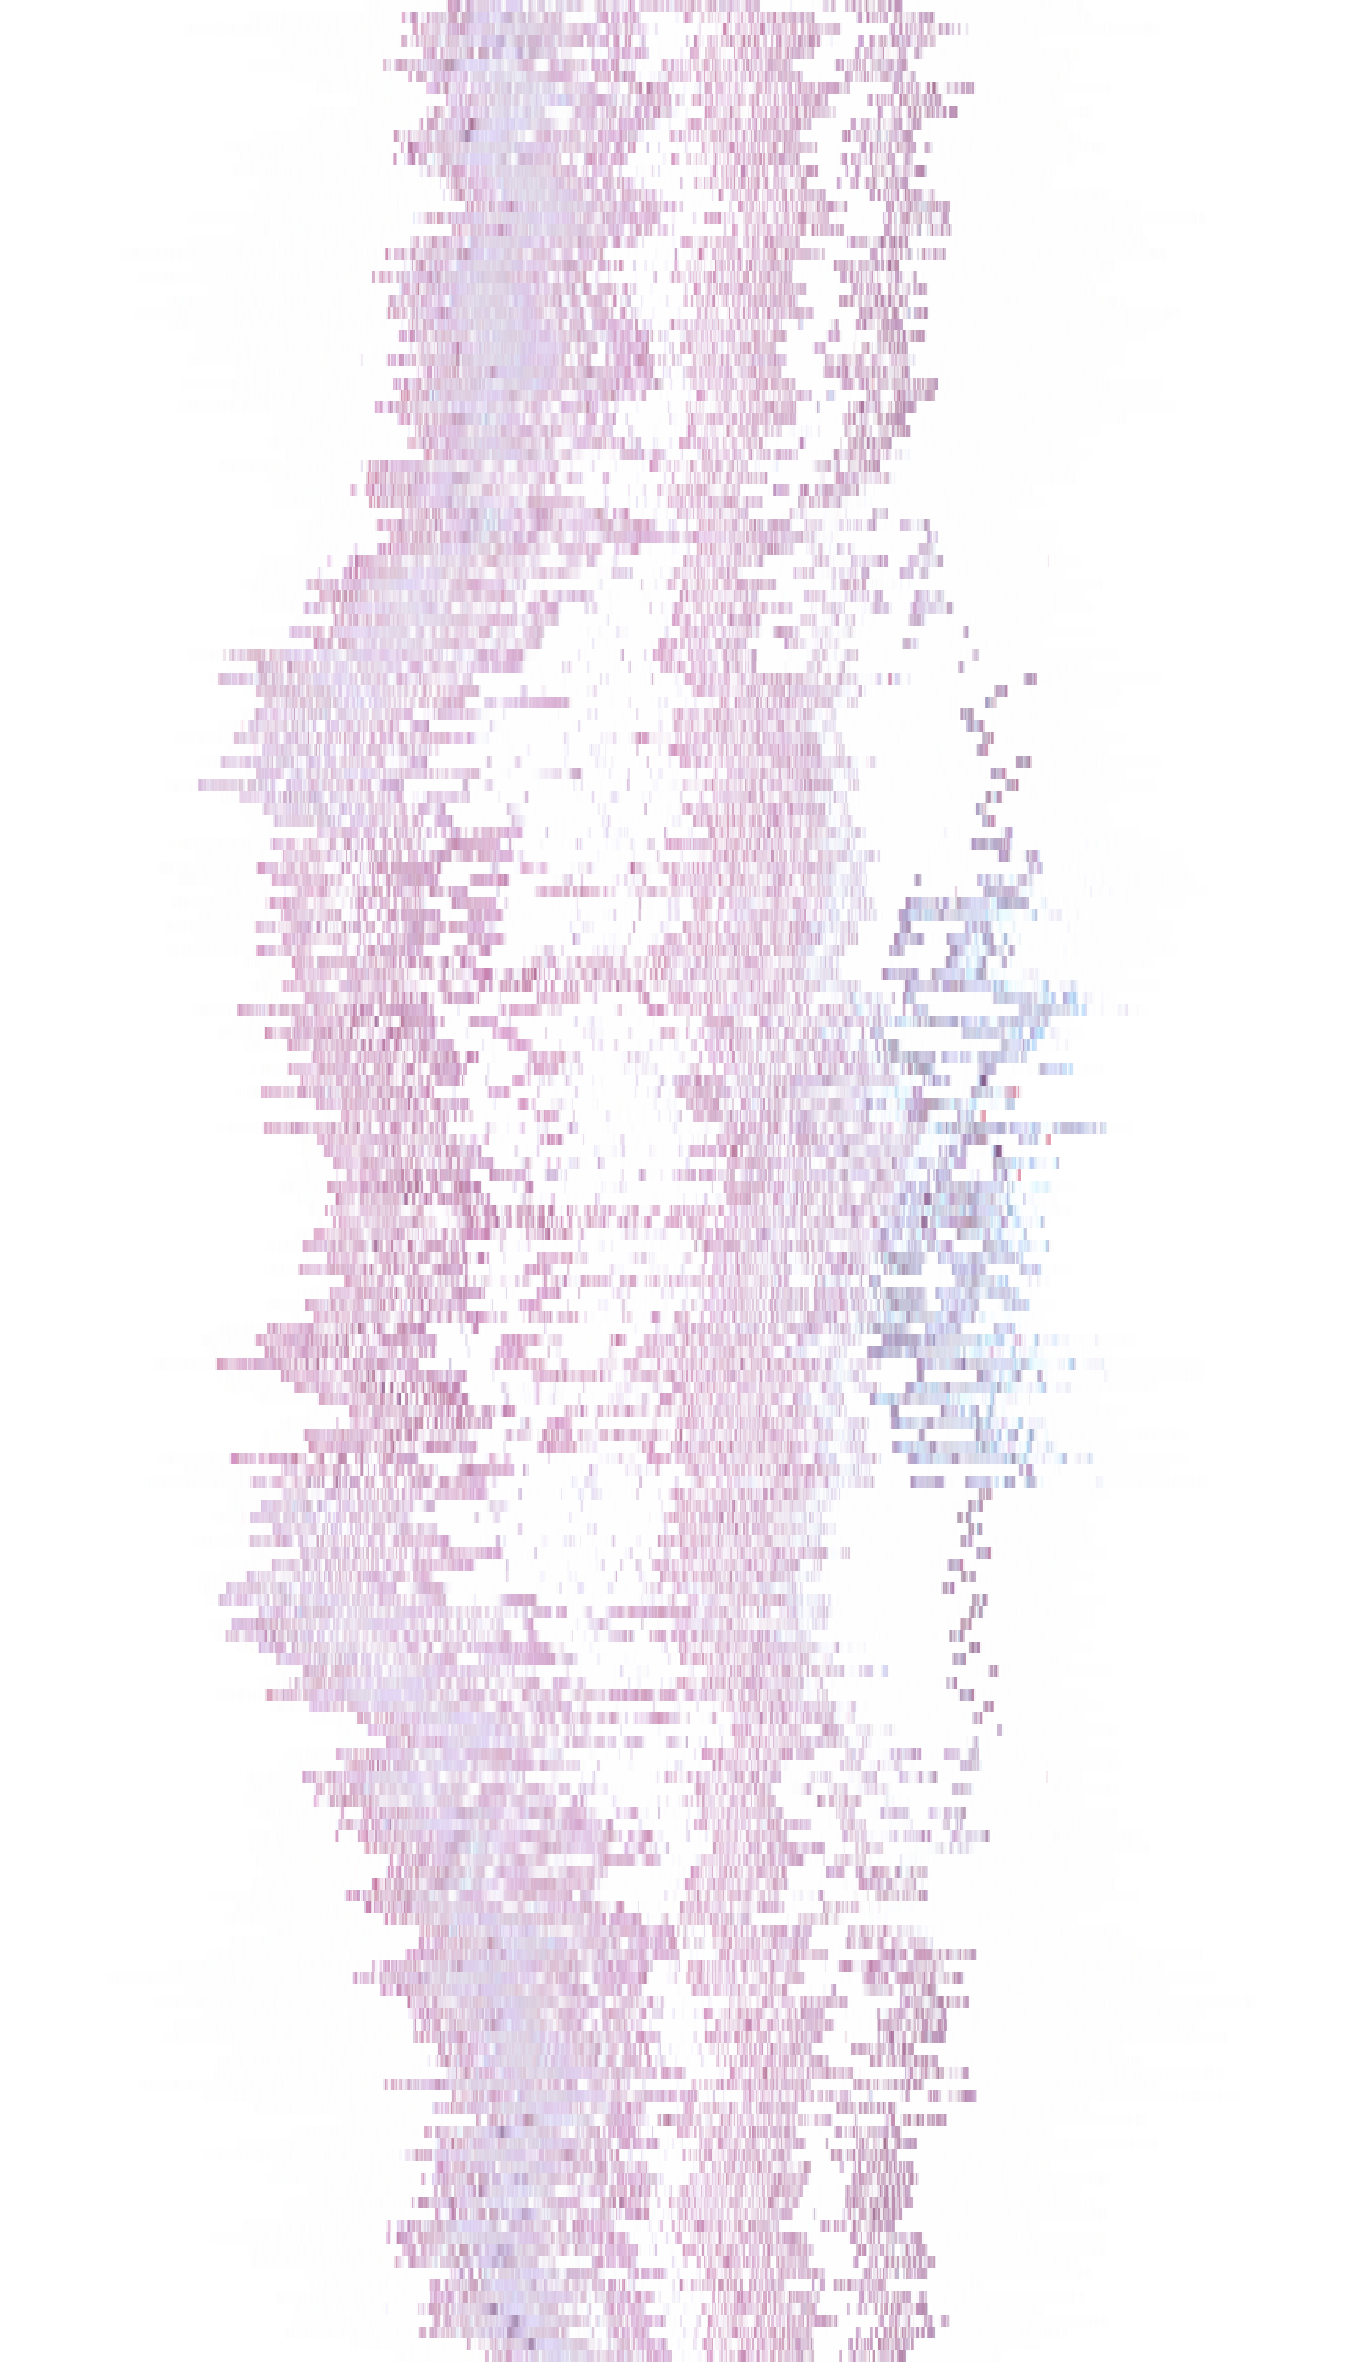
\includegraphics[height=0.4\textheight,type=pdf,ext=.pdf,read=.pdf]{Ch7/Figs/dummies/cross_section_200_alpha0.4r_1_0_352}}
    \subfigure[][3 iterations]{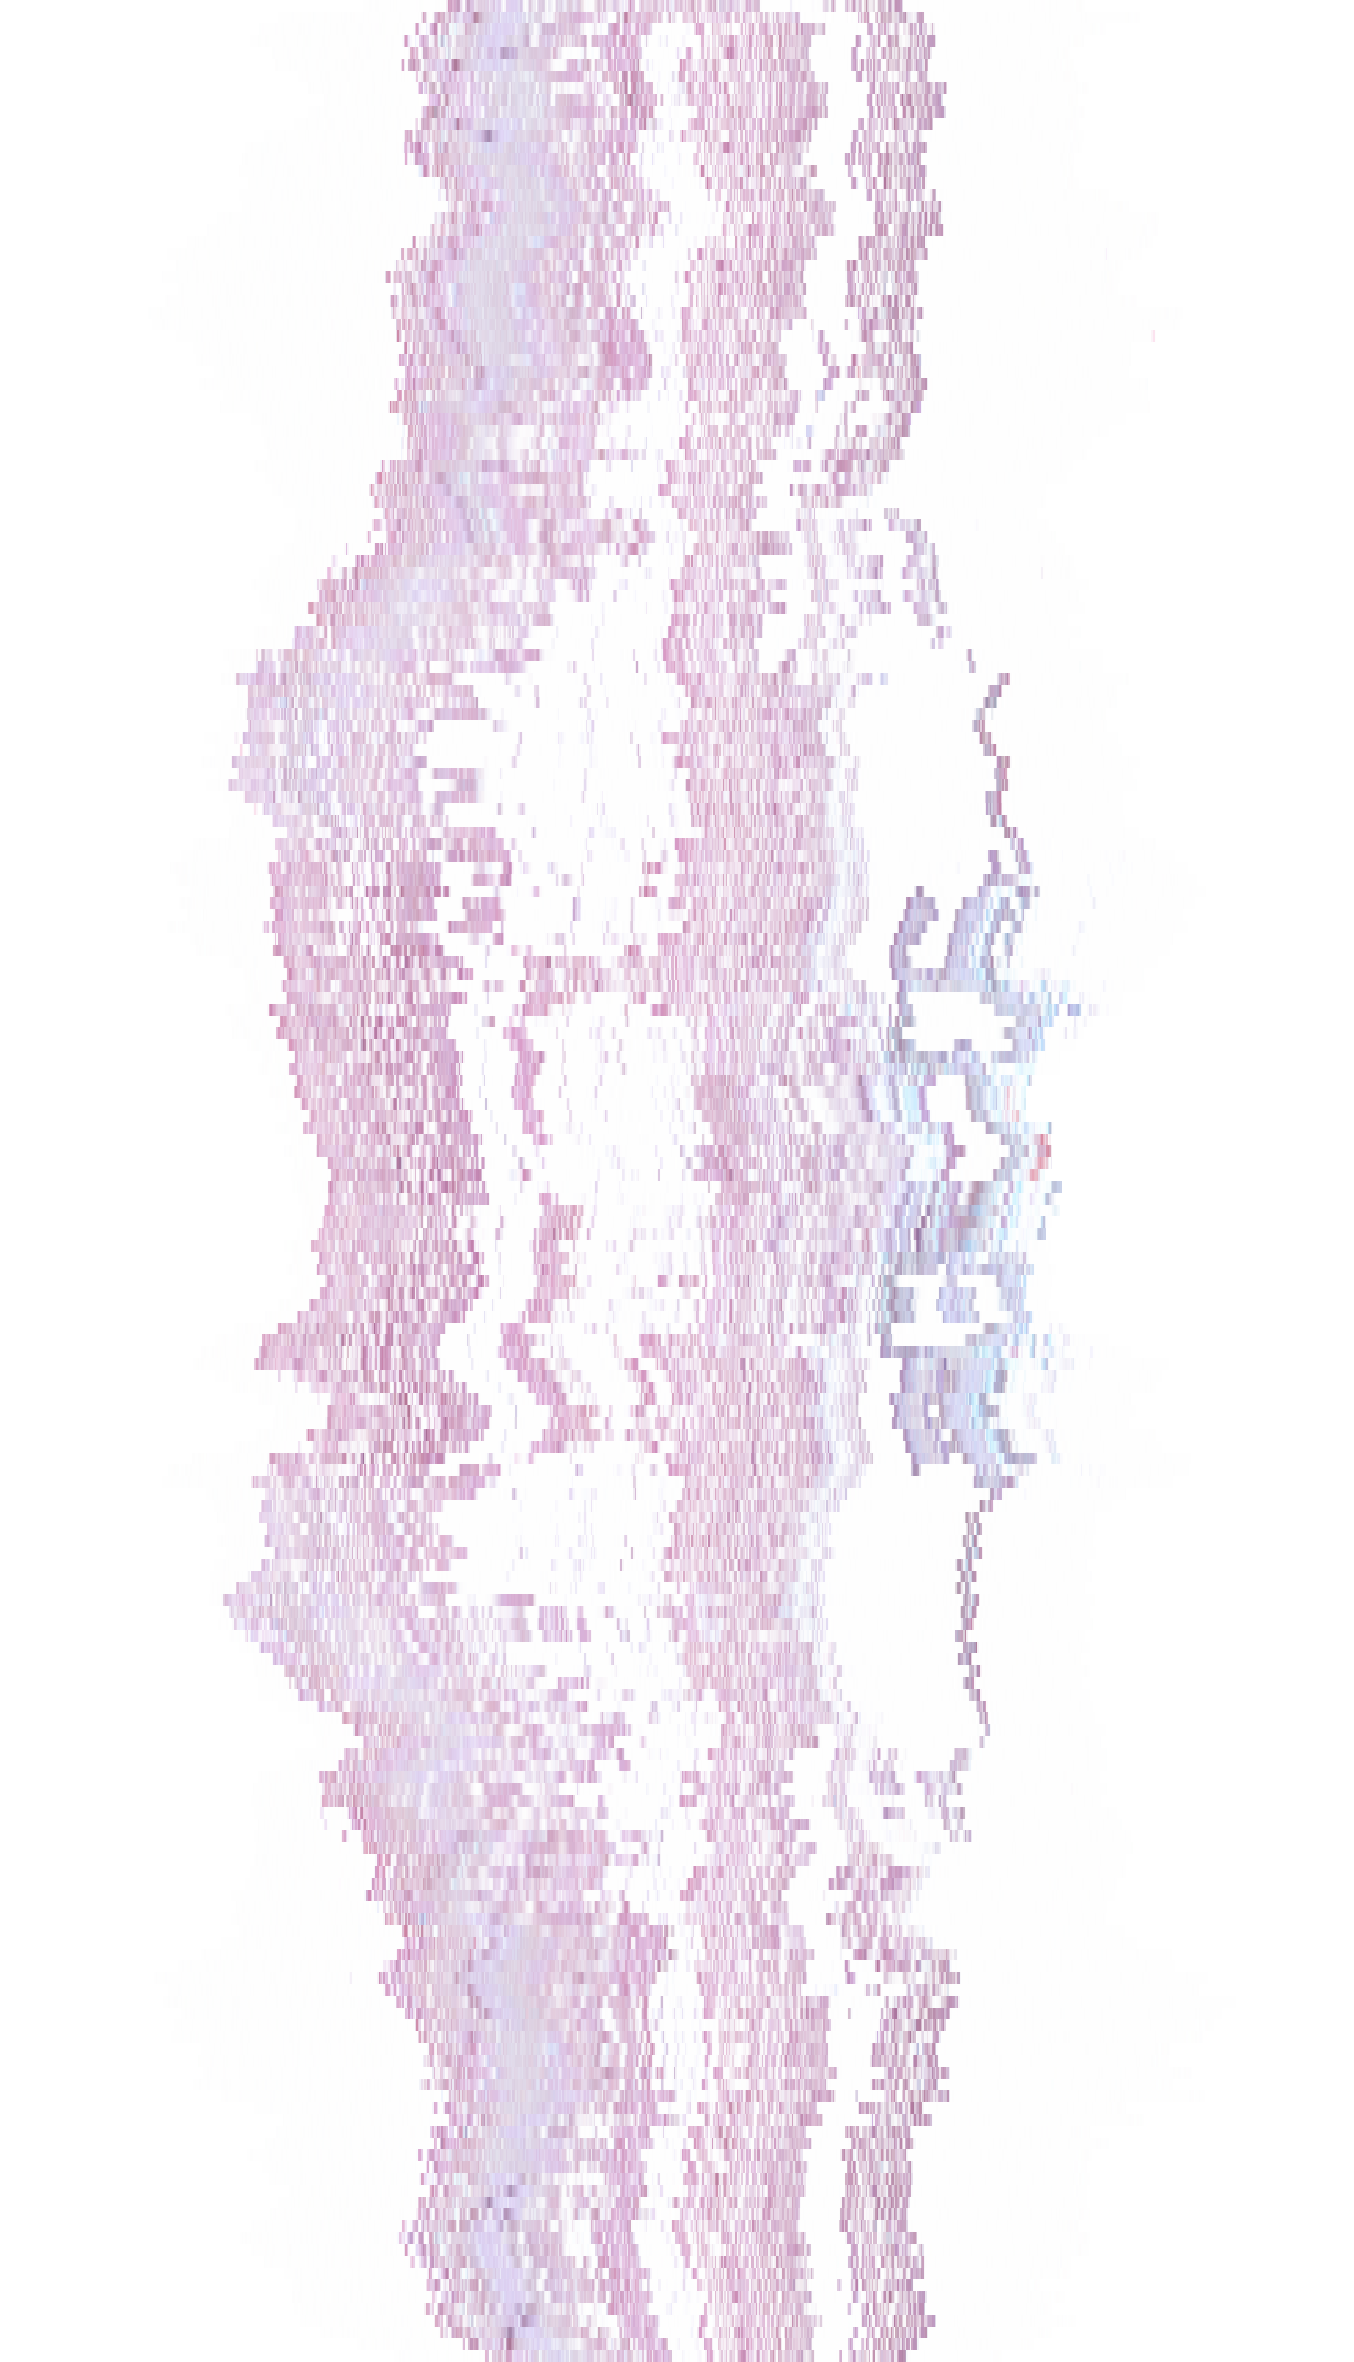
\includegraphics[height=0.4\textheight,type=pdf,ext=.pdf,read=.pdf]{Ch7/Figs/dummies/cross_section_200_alpha0.4r_3_0_352}}
    \subfigure[][8 iterations]{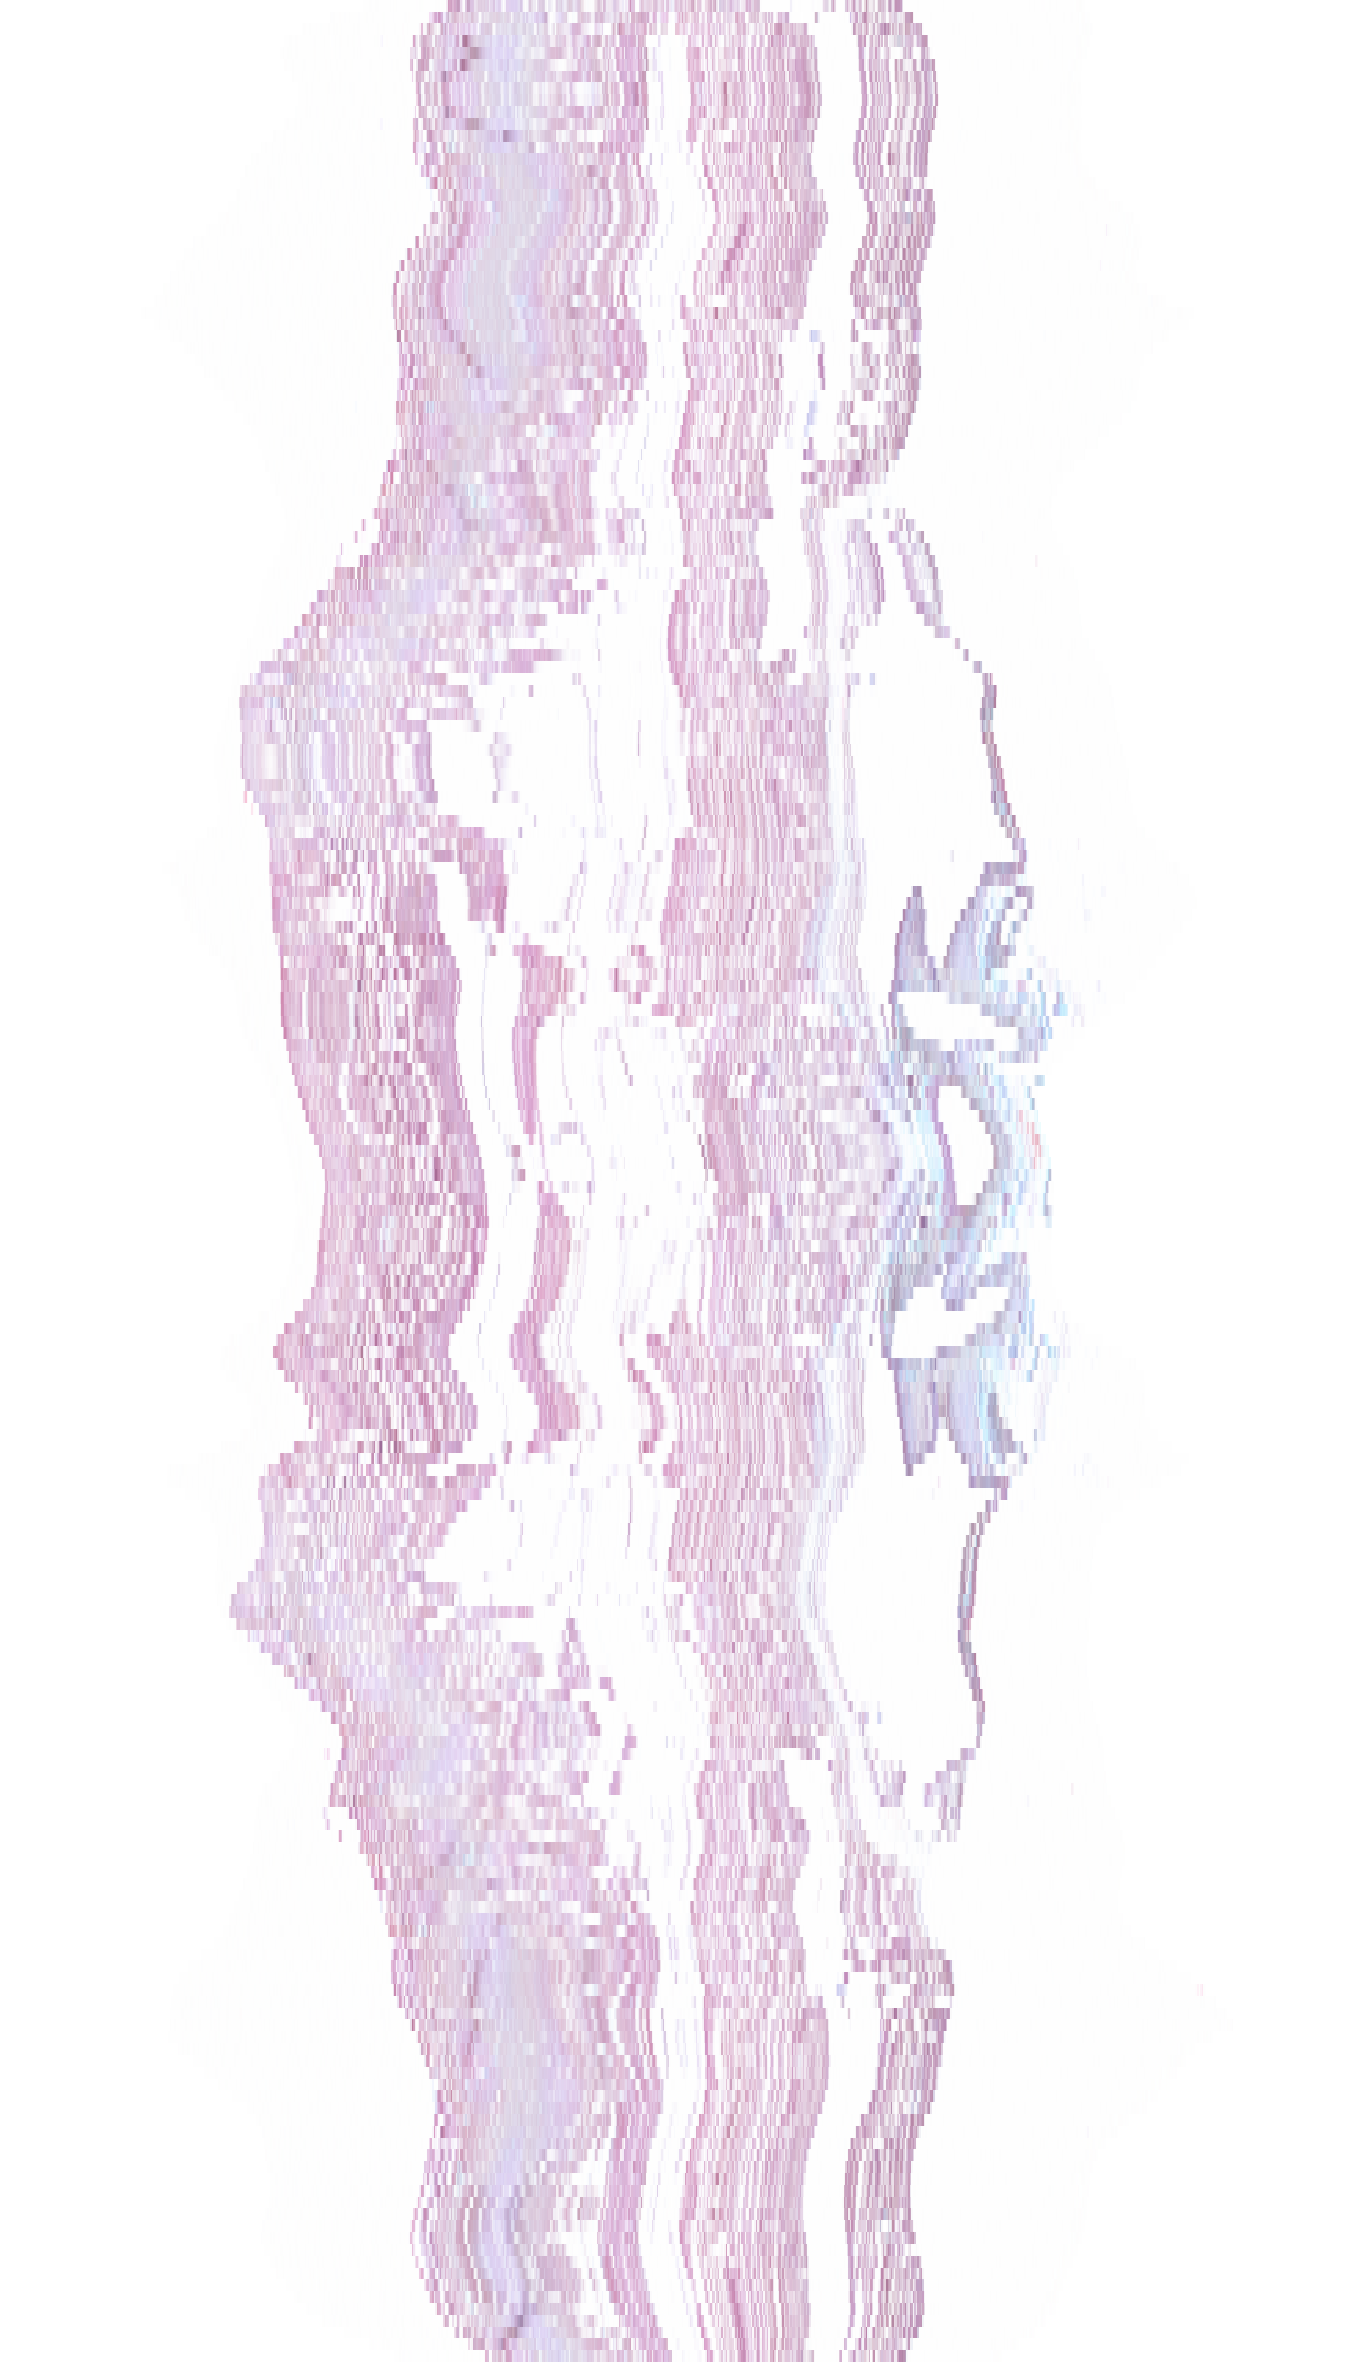
\includegraphics[height=0.4\textheight,type=pdf,ext=.pdf,read=.pdf]{Ch7/Figs/dummies/cross_section_200_alpha0.4r_8_0_352}}
    \subfigure[][20 iterations]{\includegraphics[height=0.4\textheight,type=pdf,ext=.pdf,read=.pdf]{Ch7/Figs/dummies/cross_section_200_alpha0.4r_20_0_352}}
    \subfigure[][without noise]{\includegraphics[height=0.4\textheight,type=pdf,ext=.pdf,read=.pdf]{Ch7/Figs/dummies/cross_section_perfect_200_alpha0.4r_0_352}}
    \caption{What a nice figure!}
    \label{fig:dummy_cross_sections}
  \end{figure}
  
  \begin{figure}[htbp]
    \centering
    \subfigure[][0 iterations]{\includegraphics[height=0.4\textheight,type=pdf,ext=.pdf,read=.pdf]{Ch7/Figs/dummies/cross_section_200_alpha0.4r_0_1_431}}
    \subfigure[][1 iteration]{\includegraphics[height=0.4\textheight,type=pdf,ext=.pdf,read=.pdf]{Ch7/Figs/dummies/cross_section_200_alpha0.4r_1_1_431}}
    \subfigure[][3 iterations]{\includegraphics[height=0.4\textheight,type=pdf,ext=.pdf,read=.pdf]{Ch7/Figs/dummies/cross_section_200_alpha0.4r_3_1_431}}
    \subfigure[][8 iterations]{\includegraphics[height=0.4\textheight,type=pdf,ext=.pdf,read=.pdf]{Ch7/Figs/dummies/cross_section_200_alpha0.4r_8_1_431}}
    \subfigure[][20 iterations]{\includegraphics[height=0.4\textheight,type=pdf,ext=.pdf,read=.pdf]{Ch7/Figs/dummies/cross_section_200_alpha0.4r_20_1_431}}
    \subfigure[][without noise]{\includegraphics[height=0.4\textheight,type=pdf,ext=.pdf,read=.pdf]{Ch7/Figs/dummies/cross_section_perfect_200_alpha0.4r_1_431}}
    \caption{What a nice figure!}
    \label{fig:dummy_cross_sections}
  \end{figure}
  
  % translated
  \begin{figure}[htbp]
    \centering
    \subfigure[][0 iterations]{\includegraphics[height=0.4\textheight,type=pdf,ext=.pdf,read=.pdf]{Ch7/Figs/dummies/cross_section_200_alpha0.4t_0_0_352}}
    \subfigure[][1 iteration]{\includegraphics[height=0.4\textheight,type=pdf,ext=.pdf,read=.pdf]{Ch7/Figs/dummies/cross_section_200_alpha0.4t_1_0_352}}
    \subfigure[][3 iterations]{\includegraphics[height=0.4\textheight,type=pdf,ext=.pdf,read=.pdf]{Ch7/Figs/dummies/cross_section_200_alpha0.4t_3_0_352}}
    \subfigure[][8 iterations]{\includegraphics[height=0.4\textheight,type=pdf,ext=.pdf,read=.pdf]{Ch7/Figs/dummies/cross_section_200_alpha0.4t_8_0_352}}
    \subfigure[][20 iterations]{\includegraphics[height=0.4\textheight,type=pdf,ext=.pdf,read=.pdf]{Ch7/Figs/dummies/cross_section_200_alpha0.4t_20_0_352}}
    \subfigure[][without noise]{\includegraphics[height=0.4\textheight,type=pdf,ext=.pdf,read=.pdf]{Ch7/Figs/dummies/cross_section_perfect_200_alpha0.4t_0_352}}
    \caption{What a nice figure!}
    \label{fig:dummy_cross_sections}
  \end{figure}
  
  \begin{figure}[htbp]
    \centering
    \subfigure[][0 iterations]{\includegraphics[height=0.4\textheight,type=pdf,ext=.pdf,read=.pdf]{Ch7/Figs/dummies/cross_section_200_alpha0.4t_0_1_431}}
    \subfigure[][1 iteration]{\includegraphics[height=0.4\textheight,type=pdf,ext=.pdf,read=.pdf]{Ch7/Figs/dummies/cross_section_200_alpha0.4t_1_1_431}}
    \subfigure[][3 iterations]{\includegraphics[height=0.4\textheight,type=pdf,ext=.pdf,read=.pdf]{Ch7/Figs/dummies/cross_section_200_alpha0.4t_3_1_431}}
    \subfigure[][8 iterations]{\includegraphics[height=0.4\textheight,type=pdf,ext=.pdf,read=.pdf]{Ch7/Figs/dummies/cross_section_200_alpha0.4t_8_1_431}}
    \subfigure[][20 iterations]{\includegraphics[height=0.4\textheight,type=pdf,ext=.pdf,read=.pdf]{Ch7/Figs/dummies/cross_section_200_alpha0.4t_20_1_431}}
    \subfigure[][without noise]{\includegraphics[height=0.4\textheight,type=pdf,ext=.pdf,read=.pdf]{Ch7/Figs/dummies/cross_section_perfect_200_alpha0.4t_1_431}}
    \caption{What a nice figure!}
    \label{fig:dummy_cross_sections}
  \end{figure}
    
  % rotated and translated
  \begin{figure}[htbp]
    \centering
    \subfigure[][0 iterations]{\includegraphics[height=0.4\textheight,type=pdf,ext=.pdf,read=.pdf]{Ch7/Figs/dummies/cross_section_200_alpha0.4rt_0_0_352}}
    \subfigure[][1 iteration]{\includegraphics[height=0.4\textheight,type=pdf,ext=.pdf,read=.pdf]{Ch7/Figs/dummies/cross_section_200_alpha0.4rt_1_0_352}}
    \subfigure[][3 iterations]{\includegraphics[height=0.4\textheight,type=pdf,ext=.pdf,read=.pdf]{Ch7/Figs/dummies/cross_section_200_alpha0.4rt_3_0_352}}
    \subfigure[][8 iterations]{\includegraphics[height=0.4\textheight,type=pdf,ext=.pdf,read=.pdf]{Ch7/Figs/dummies/cross_section_200_alpha0.4rt_8_0_352}}
    \subfigure[][20 iterations]{\includegraphics[height=0.4\textheight,type=pdf,ext=.pdf,read=.pdf]{Ch7/Figs/dummies/cross_section_200_alpha0.4rt_20_0_352}}
    \subfigure[][without noise]{\includegraphics[height=0.4\textheight,type=pdf,ext=.pdf,read=.pdf]{Ch7/Figs/dummies/cross_section_perfect_200_alpha0.4rt_0_352}}
    \caption{What a nice figure! Notice a quarter of the way up from the base, a bad registration between 1 and 3 has been corrected in 10.}
    \label{fig:dummy_cross_sections}
  \end{figure}
  
  \begin{figure}[htbp]
    \centering
    \subfigure[][0 iterations]{\includegraphics[height=0.4\textheight,type=pdf,ext=.pdf,read=.pdf]{Ch7/Figs/dummies/cross_section_200_alpha0.4rt_0_1_431}}
    \subfigure[][1 iteration]{\includegraphics[height=0.4\textheight,type=pdf,ext=.pdf,read=.pdf]{Ch7/Figs/dummies/cross_section_200_alpha0.4rt_1_1_431}}
    \subfigure[][3 iterations]{\includegraphics[height=0.4\textheight,type=pdf,ext=.pdf,read=.pdf]{Ch7/Figs/dummies/cross_section_200_alpha0.4rt_3_1_431}}
    \subfigure[][8 iterations]{\includegraphics[height=0.4\textheight,type=pdf,ext=.pdf,read=.pdf]{Ch7/Figs/dummies/cross_section_200_alpha0.4rt_8_1_431}}
    \subfigure[][20 iterations]{\includegraphics[height=0.4\textheight,type=pdf,ext=.pdf,read=.pdf]{Ch7/Figs/dummies/cross_section_200_alpha0.4rt_20_1_431}}
    \subfigure[][without noise]{\includegraphics[height=0.4\textheight,type=pdf,ext=.pdf,read=.pdf]{Ch7/Figs/dummies/cross_section_perfect_200_alpha0.4rt_1_431}}
    \caption{What a nice figure! Notice a quarter of the way up from the base, a bad registration between 1 and 3 has been corrected in 10}
    \label{fig:dummy_cross_sections}
  \end{figure}
  
  % mean squared differences 3D
  \begin{sidewaysfigure}[htbp]
    \centering
    \subfigure[][straight column]{\includegraphics[height=0.33\textheight,type=pdf,ext=.pdf,read=.pdf]{Ch7/Figs/dummies/segmentation_mean_square_differences_3D}}
    \subfigure[][rotation]{\includegraphics[height=0.33\textheight,type=pdf,ext=.pdf,read=.pdf]{Ch7/Figs/dummies/segmentation_mean_square_differences_3Dr}}
    \subfigure[][translation]{\includegraphics[height=0.33\textheight,type=pdf,ext=.pdf,read=.pdf]{Ch7/Figs/dummies/segmentation_mean_square_differences_3Dt}}
    \subfigure[][rotation and translation]{\includegraphics[height=0.33\textheight,type=pdf,ext=.pdf,read=.pdf]{Ch7/Figs/dummies/segmentation_mean_square_differences_3Drt}}
    \caption{3D evolution of mean squared difference. Discuss how, as is visible in the colour and segmentation mean squared difference slices, even though registration was performed with the colour image, mean squared differences were calculated with the segmentation, and the results are much less noisy and clearer. Discuss how boundary conditions mean edges are diffused like at the back of b, and how mistakes are robust like the spike in a.}
    \label{fig:dummy_cross_sections}
  \end{sidewaysfigure}
  
  % mean squared differences 2D
  \begin{sidewaysfigure}[htbp]
    \centering
    \subfigure[][straight column]{\includegraphics[height=0.33\textheight,type=pdf,ext=.pdf,read=.pdf]{Ch7/Figs/dummies/segmentation_mean_square_differences_2D}}
    \subfigure[][rotation]{\includegraphics[height=0.33\textheight,type=pdf,ext=.pdf,read=.pdf]{Ch7/Figs/dummies/segmentation_mean_square_differences_2Dr}}
    \subfigure[][translation]{\includegraphics[height=0.33\textheight,type=pdf,ext=.pdf,read=.pdf]{Ch7/Figs/dummies/segmentation_mean_square_differences_2Dt}}
    \subfigure[][rotation and translation]{\includegraphics[height=0.33\textheight,type=pdf,ext=.pdf,read=.pdf]{Ch7/Figs/dummies/segmentation_mean_square_differences_2Drt}}
    \caption{Comment on magnitude and spectrum of error (higher frequencies filtered out)}
    \label{fig:dummy_cross_sections}
  \end{sidewaysfigure}
    
  this is a load of content
  
  this is a load of content
  
  this is a load of content
  
  this is a load of content
  
  this is a load of content
  
  this is a load of content
  
  this is a load of content
  
  this is a load of content
  
  this is a load of content
  
  this is a load of content
  
  this is a load of content
  
  this is a load of content
  
  % old result
  \begin{sidewaysfigure}[htbp]
    \centering
    \subfigure[][0 iterations]{\includegraphics[height=0.33\textheight,type=pdf,ext=.pdf,read=.pdf]{Ch7/Figs/dummies/low_noise_with_original_images_cross_section_200_alpha0.4rt_0_0_088}}
    \subfigure[][1 iteration]{\includegraphics[height=0.33\textheight,type=pdf,ext=.pdf,read=.pdf]{Ch7/Figs/dummies/low_noise_with_original_images_cross_section_200_alpha0.4rt_1_0_088}}
    \subfigure[][3 iterations]{\includegraphics[height=0.33\textheight,type=pdf,ext=.pdf,read=.pdf]{Ch7/Figs/dummies/low_noise_with_original_images_cross_section_200_alpha0.4rt_3_0_088}}
    \subfigure[][10 iterations]{\includegraphics[height=0.33\textheight,type=pdf,ext=.pdf,read=.pdf]{Ch7/Figs/dummies/low_noise_with_original_images_cross_section_200_alpha0.4rt_10_0_088}}
    \subfigure[][without noise]{\includegraphics[height=0.33\textheight,type=pdf,ext=.pdf,read=.pdf]{Ch7/Figs/dummies/low_noise_with_original_images_cross_section_perfect_200_alpha0.4rt_0_088}}
    \caption{What a nice figure! Notice a quarter of the way up from the base, a bad registration between 1 and 3 has been corrected in 10. This demonstrates that even when the cost function of the registration is spiky, and results of a single run are sensitive to initialisation, the iterative nature of the diffusion algorithm greatly improves robustness by providing multiple opportunities to escape local minima.}
    \label{fig:dummy_cross_sections}
  \end{sidewaysfigure}
  
  
  % full contours
  \begin{figure}[htbp]\texttt{}
    \centering
    \subfigure[][]{\includegraphics[width=0.3\pagewidth]{Ch7/Figs/dummies/contours/whole_surface_0}}
    \subfigure[][]{\includegraphics[width=0.3\pagewidth]{Ch7/Figs/dummies/contours/whole_surface_1}}
    \subfigure[][]{\includegraphics[width=0.3\pagewidth]{Ch7/Figs/dummies/contours/whole_surface_3}}
    \subfigure[][]{\includegraphics[width=0.3\pagewidth]{Ch7/Figs/dummies/contours/whole_surface_8}}
    \subfigure[][]{\includegraphics[width=0.3\pagewidth]{Ch7/Figs/dummies/contours/whole_surface_20}}
    \caption{What a nice figure!}
    \label{fig:test.png}
  \end{figure}
  
  \begin{figure}[htbp]
    \centering
    \subfigure[][]{\includegraphics[width=0.3\pagewidth]{Ch7/Figs/dummies/contours/whole_surfacer_0}}
    \subfigure[][]{\includegraphics[width=0.3\pagewidth]{Ch7/Figs/dummies/contours/whole_surfacer_1}}
    \subfigure[][]{\includegraphics[width=0.3\pagewidth]{Ch7/Figs/dummies/contours/whole_surfacer_3}}
    \subfigure[][]{\includegraphics[width=0.3\pagewidth]{Ch7/Figs/dummies/contours/whole_surfacer_8}}
    \subfigure[][]{\includegraphics[width=0.3\pagewidth]{Ch7/Figs/dummies/contours/whole_surfacer_20}}
    \caption{What a nice figure!}
    \label{fig:test.png}
  \end{figure}
  
  \begin{figure}[htbp]
    \centering
    \subfigure[][]{\includegraphics[width=0.3\pagewidth]{Ch7/Figs/dummies/contours/whole_surfacet_0}}
    \subfigure[][]{\includegraphics[width=0.3\pagewidth]{Ch7/Figs/dummies/contours/whole_surfacet_1}}
    \subfigure[][]{\includegraphics[width=0.3\pagewidth]{Ch7/Figs/dummies/contours/whole_surfacet_3}}
    \subfigure[][]{\includegraphics[width=0.3\pagewidth]{Ch7/Figs/dummies/contours/whole_surfacet_8}}
    \subfigure[][]{\includegraphics[width=0.3\pagewidth]{Ch7/Figs/dummies/contours/whole_surfacet_20}}
    \caption{What a nice figure!}
    \label{fig:test.png}
  \end{figure}
  
  \begin{figure}[htbp]
    \centering
    \subfigure[][]{\includegraphics[width=0.3\pagewidth]{Ch7/Figs/dummies/contours/whole_surfacert_0}}
    \subfigure[][]{\includegraphics[width=0.3\pagewidth]{Ch7/Figs/dummies/contours/whole_surfacert_1}}
    \subfigure[][]{\includegraphics[width=0.3\pagewidth]{Ch7/Figs/dummies/contours/whole_surfacert_3}}
    \subfigure[][]{\includegraphics[width=0.3\pagewidth]{Ch7/Figs/dummies/contours/whole_surfacert_8}}
    \subfigure[][]{\includegraphics[width=0.3\pagewidth]{Ch7/Figs/dummies/contours/whole_surfacert_20}}
    \caption{This is a figure!}
    \label{fig:test.png}
  \end{figure}
  
  It is worth noting that the adjustment algorithm itself is stable with much larger levels of noise than shown here, comparable to those in Figures~\ref{fig:1d_diffusion_0_40}, \ref{fig:1d_diffusion_0_49}, \ref{fig:1d_diffusion_0_50} and \ref{fig:1d_diffusion_0_51}. It is simply that the registration is sensitive, wouldn't work blah blah.
  
  Parameters used for noisy dummies were x, y, z. The important factor is whether the slice-to-slice registrations are quickly and robustly successful, and so much greater noise could be filtered by the algorithm, as long as the parameters were tuned for large displacements for the first few iterations, and then smaller displacements for the finer smoothing in the later iterations.
  
  Prove that random walk is binomial distribution, which tends to Gaussian distribution, therefore with enough iterations we are applying gaussian transformational smoothing to the volume.
  
  Particles undergoing brownian motion diffuse, hence the name.
  
  % `http://en.wikipedia.org/wiki/Random_walk#One-dimensional_random_walk'
  1D analogy of diffusion and noise filtering, with sine wave and overlayed noise, and diagram
  
  Figure of banana-effect registration
  
  Anisotropic diffusion: 
  
  Divide MRI into slices, then apply artificial noise, then compare banana registration to diffusion registration.
  
  Pull image from Evernote
  
  \subsection{2D Transforms Diffusion} % (fold)
  \label{sub:2d_transforms_diffusion}
    This 1-dimensional model is trivially extended to a 2D translation of a slice image aligning with its neighbour, since both of the parameters are mutually orthogonal. But what about the more complex harder with say affine transform. Square root of transform blah blah.
  
  % subsection 2d_transforms_diffusion (end)
  
% section methods (end)

\section{Results} % (fold)
\label{sec:results}
  
  Figures:
  
  % x slices
  \begin{figure}[htbp]
    \centering
    \subfigure[][]{\includegraphics[height=0.31\textheight]{Ch7/Figs/adjusted_0_0_235}}
    \subfigure[][]{\includegraphics[height=0.31\textheight]{Ch7/Figs/adjusted_1_0_235}}
    \subfigure[][]{\includegraphics[height=0.31\textheight]{Ch7/Figs/adjusted_20_0_235}}
    \caption{Cross-section after 0, 1 and 20 iterations of diffusion}
    \label{fig:adjusted_0_235}
  \end{figure}

  % y slices
  \begin{figure}[htbp]
    \centering
    \subfigure[][]{\includegraphics[height=0.31\textheight]{Ch7/Figs/adjusted_0_1_287}}
    \subfigure[][]{\includegraphics[height=0.31\textheight]{Ch7/Figs/adjusted_1_1_287}}
    \subfigure[][]{\includegraphics[height=0.31\textheight]{Ch7/Figs/adjusted_20_1_287}}
    \caption{Cross-section after 0, 1 and 20 iterations of diffusion}
    \label{fig:adjusted_1_287}
  \end{figure}
  
  % lower 100 slices zoom
  % x slices
  \begin{sidewaysfigure}[htbp]
    \centering
    \subfigure[][]{\includegraphics[height=0.15\textheight]{Ch7/Figs/adjusted_0_0_235_zoomed}}
    \subfigure[][]{\includegraphics[height=0.15\textheight]{Ch7/Figs/adjusted_1_0_235_zoomed}}
    \subfigure[][]{\includegraphics[height=0.15\textheight]{Ch7/Figs/adjusted_20_0_235_zoomed}}
    \caption{Lower 100 slices of cross-section after 0, 1 and 20 iterations of diffusion}
    \label{fig:adjusted_0_235}
  \end{sidewaysfigure}

  % y slices
  \begin{sidewaysfigure}[htbp]
    \centering
    \subfigure[][]{\includegraphics[height=0.15\textheight]{Ch7/Figs/adjusted_0_1_287_zoomed}}
    \subfigure[][]{\includegraphics[height=0.15\textheight]{Ch7/Figs/adjusted_1_1_287_zoomed}}
    \subfigure[][]{\includegraphics[height=0.15\textheight]{Ch7/Figs/adjusted_20_1_287_zoomed}}
    \caption{Lower 100 slices of cross-section after 0, 1 and 20 iterations of diffusion}
    \label{fig:adjusted_1_287}
  \end{sidewaysfigure}
  
  % diffused contours
  \begin{sidewaysfigure}[p]
    \centering
    \subfigure[][]{\includegraphics[width=0.9\textheight]{Ch7/Figs/Rat28/contours/whole_positive_x_diffused}}
    \caption{}
    \label{fig:image1.png}
  \end{sidewaysfigure}

  \begin{sidewaysfigure}[p]
    \centering
    \subfigure[][]{\includegraphics[width=0.9\textheight]{Ch7/Figs/Rat28/contours/whole_negative_x_diffused}}
    \caption{}
    \label{fig:image1.png}
  \end{sidewaysfigure}

  \begin{sidewaysfigure}[p]
    \centering
    \subfigure[][]{\includegraphics[width=0.9\textheight]{Ch7/Figs/Rat28/contours/whole_positive_y_diffused}}
    \caption{}
    \label{fig:image1.png}
  \end{sidewaysfigure}

  \begin{sidewaysfigure}[p]
    \centering
    \subfigure[][]{\includegraphics[width=0.9\textheight]{Ch7/Figs/Rat28/contours/whole_positive_z_diffused}}
    \caption{}
    \label{fig:image1.png}
  \end{sidewaysfigure}

  
  
  2 cross-sections and a contour surface of:
    the straight column, rotation, translation, rotation + translation volumes
      with perfect, noisy, smoothed 0.4, smoothed 0.3
        
  Figure of 0.4 200rt plot\_metric\_values\_and\_differences from the first step, showing that all the registrations are reaching their minimum of around the same low metric value, it's just that the computation of the Adjusted Transforms is unstable.
  
  
  
  
  \subsection{Regional Registration} % (fold)
  \label{sub:regional_registration}
    Segment a largish blood vessel or vessel branch in the histology and show that it looks like a smooth surface and is aligned. 
  % subsection regional_registration (end)

% section results (end)

\section{Discussion} % (fold)
\label{sec:discussion}
  GENERAL POINT, `it will be shown later' in introductory paragraphs, to tittilate the reader.
  
  With a better interpolation scheme, it might be possible to crank alpha up further.
  
  Inherently introduces the banana problem across the curvature of the heart (~30 slices - give justification with numbers)
  Can only be used for small adjustments, given non-commutativity of operators etc.
  Figures and evaluation of results e.g. examples of great and bad slice-pair registrations, maybe one slice has a large abberation. Works better for different regions? e.g. round blob versus cavity?
  Alternative Implementations:
  Could register to more than just nearest neighbours at each iteration, although multiple iterations of nearest neighbour is equivalent to this, requires the same total number of slice-to-slice iterations, and is more stable and accurate, as errors from the first nearest neighbour iteration due to e.g. interpolation error, random noise etc. are mitigated by subsequent iterations.
  Expensive to rerun slice-pair registrations every iteration, could infer from previous registration. Inaccuracy and instability?
  
  Could be extended easily to more complex transforms such as b-spline, although perhaps a little trickier to think about interpolating transforms other than linearly interpolating their parameters.
  
  More robust than even banana registration, as images have many chances to jump out from local minima.

% section discussion (end)

% chapter diffusion_smoothing_registration_of_high_resolution_rat_histology (end)
